\documentclass{article}
\usepackage{geometry}
\usepackage{amssymb}
\usepackage{xcolor}
\usepackage{booktabs}
\usepackage{graphicx}
\usepackage{float}
\usepackage{caption}
\usepackage[italian]{babel}

\setcounter{page}{0}

% Set the desired margins
\geometry{
    left=.7in,   % Left margin
    right=.7in,  % Right margin
    top=.7in,    % Top margin
    bottom=.7in, % Bottom margin
}


\title{Materiali per l'elettronica con laboratorio}
\author{Gruppo 4: Francesca Capellino, Alessio Cimma, Sexhei Lala}


\begin{document}

\maketitle

\begin{center}
    \includegraphics*[width=0.22\linewidth]{../images/logo.png}
\end{center}

\tableofcontents

\newpage
Nota: In tutti i grafici sono stati riportati i $\chi^2$ ridotti, che per brevità sono stati chiamati $\chi^2$ e basta. La scelta è stata giustificata con la necessità di tenere in considerazione che i dati analizzati sono vincolati da una funzione teorica, e non sono sample statistici.
\section{Caratterizzazione di Diodi e LED}

\subsection{Caratterizzazione elettrica di resistenze lineari}

\subsubsection{Scopo dell'esperienza}

Lo scopo di questa prima esperienza è stato di acquisire familiarità con la strumentazione e verificare la corretta calibrazione degli strumenti tramite una retta di taratura: nel circuito che abbiamo costruito era presente una resistenza ohmica, per cui ci aspettavamo un andamento del tipo $R=\frac{V}{I}$. 

\subsubsection{Strumentazione}

\begin{itemize} 
    \item Voltmetro AMPROBE 37XR-A
    \item Generatore di tensione GWINSTEK GPS-4303 
    \item Amperometro RSPRO IDM 103N (modalità fast)
    \item Universal Breadboard
    \item Cablaggio
    \item Resistenza da $10.0\pm0.5 k \Omega$
    \item sensibilità voltmetro: $\pm0.1\% + 5 dgts$
    \item sensibilità amperometro: $\pm0.6\%+2 dgts$
\end{itemize}

\subsubsection{Procedimento}

\begin{figure}[h]
    \begin{minipage}{0.7\textwidth} % Adjust the width as needed
        Abbiamo realizzato il circuito come in Figura \ref{circuito:1} usando una resistenza ($R=10k\Omega$) . Abbiamo affettuato una serie di misure della corrente I in funzione della tensione V (letta sul voltmetro) e abbiamo ottenuto i valori riportati in appendice nella tabella \ref{tab:tabella1}.
    \end{minipage}
    \hfill % Add horizontal space between minipages
    \begin{minipage}{0.25\textwidth} % Adjust the width as needed
        \centering
        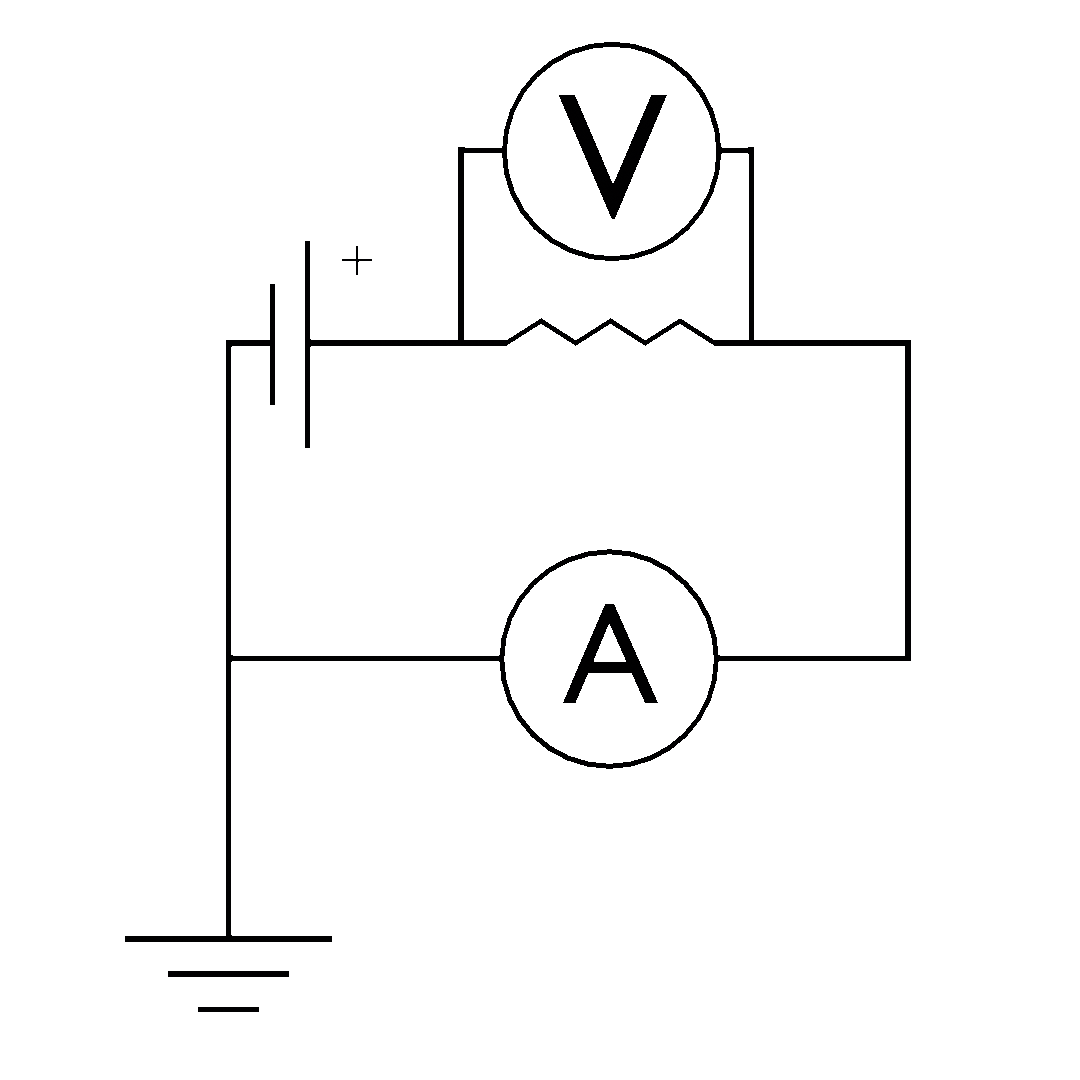
\includegraphics[width=\linewidth]{../images/circuito1.png} % Replace example-image with your figure filename
        \caption{circuito per caratterizzazione di una resistenza}
        \label{circuito:1}
    \end{minipage}
\end{figure}

\newpage

\subsubsection{Analisi dati}
Abbiamo effettuato un fit lineare dei dati precedenti con la funzione interpolante $y=ax+b$ da cui abbiamo ricavato, tramite la legge di Ohm $I=\frac{V}{R}$ (dove $V$ è la tensione applicata, $R$ è la resistenza del circuito e $I$ è la corrente che passa attraverso) che la pendenza della retta interpolante $a$ corrisponde a $\frac{1}{R}$, per cui:
\begin{figure}[h]
    \begin{minipage}{0.69\textwidth} % Adjust the width as needed
        \centering
        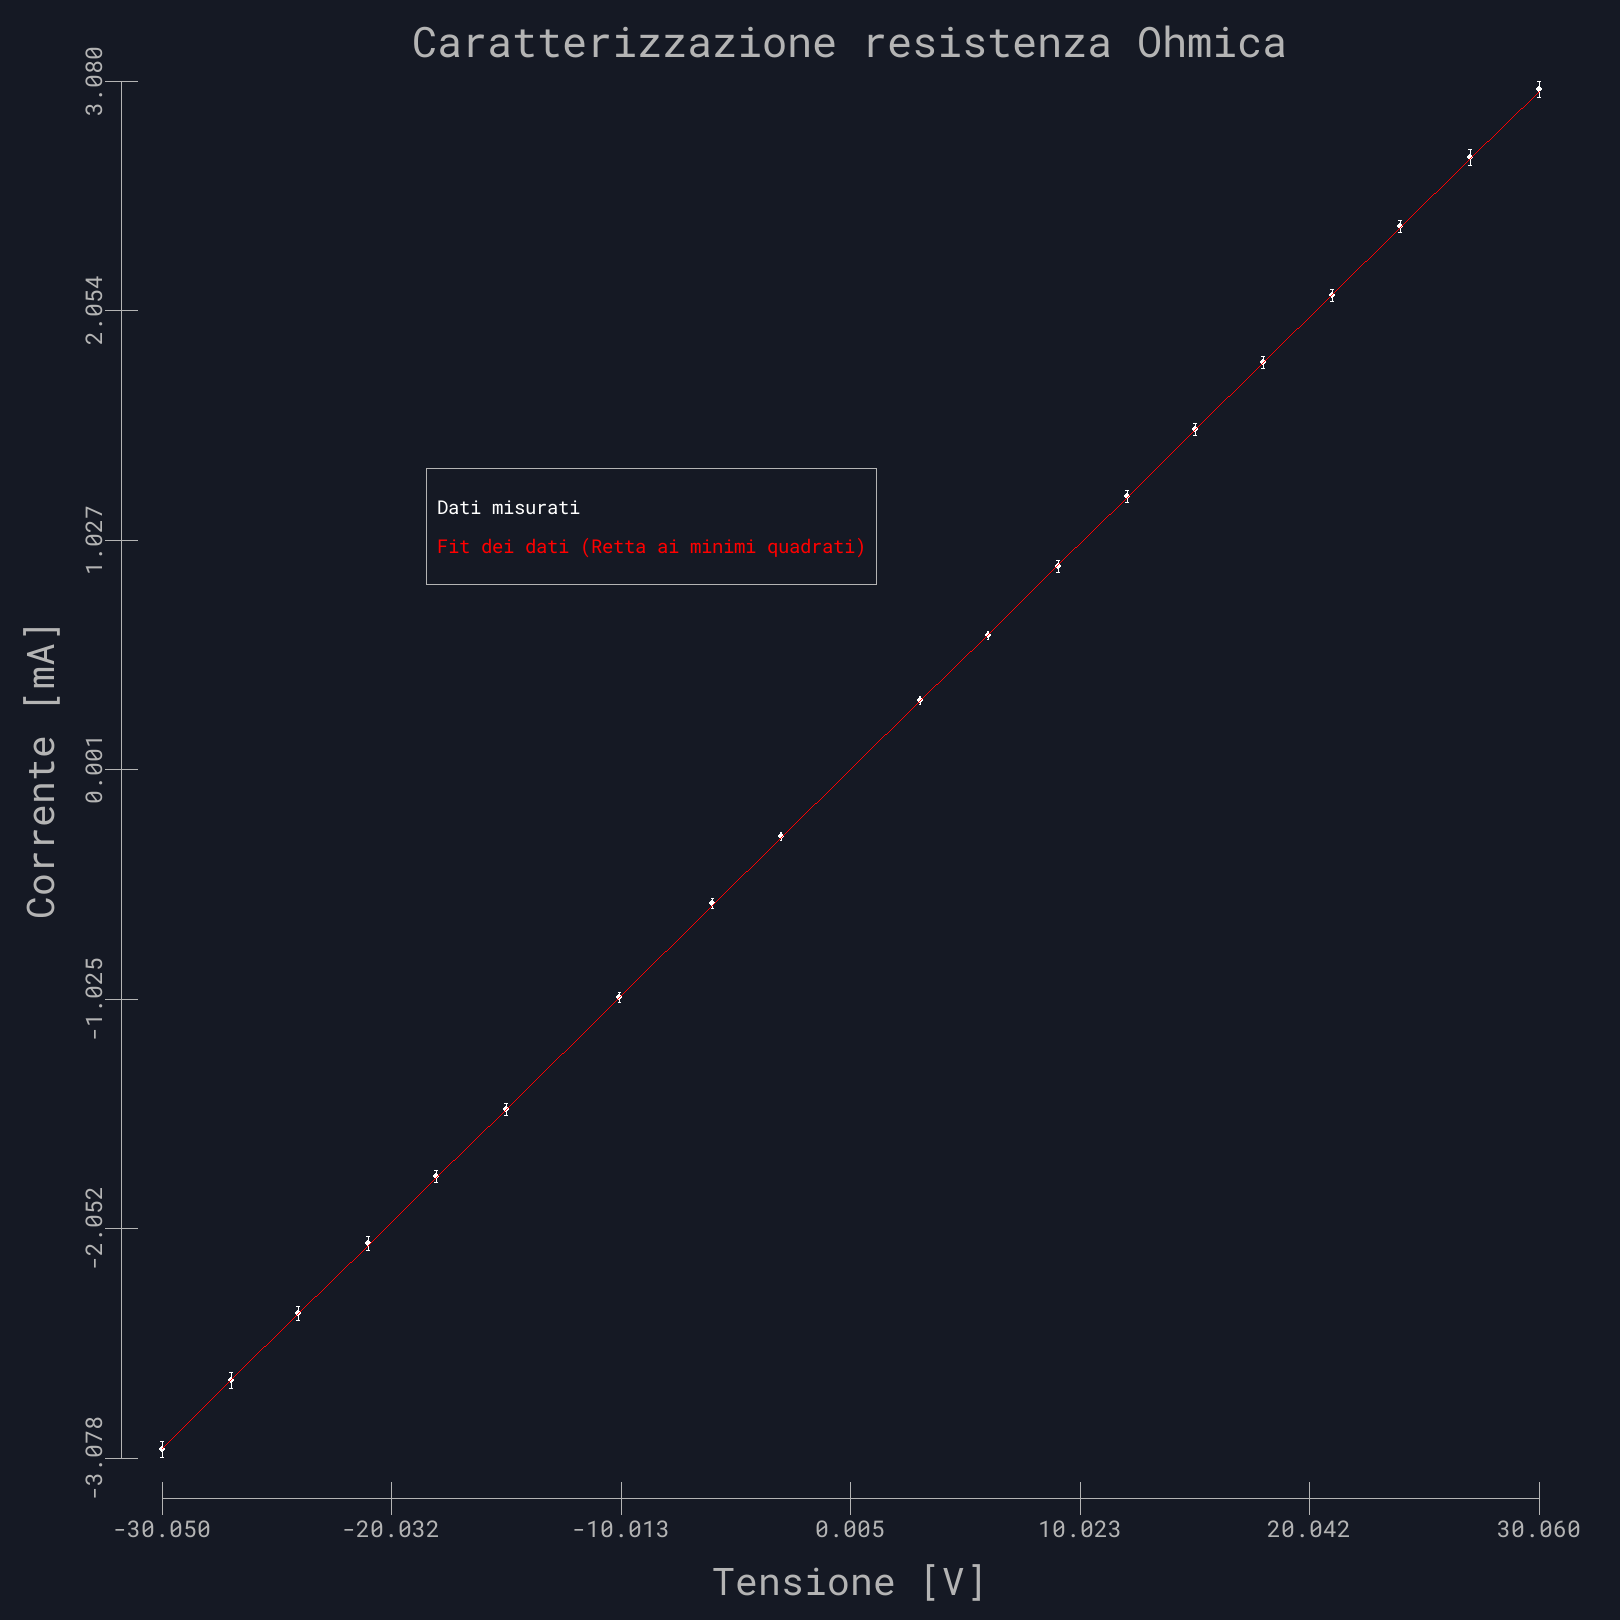
\includegraphics[width=\linewidth]{../images/grafico1.png} % Replace example-image with your figure filename
        \caption{Retta di taratura della resistenza ohmica}
        \label{grafico:1}
    \end{minipage}
    \hfill % Add horizontal space between minipages
    \begin{minipage}{0.3\textwidth}    
    \begin{itemize}
        \item $a=(0.10055\pm 4*10^{-5} )k\Omega^{-1}$
        \item $b=(0.0007 \pm 0.0007)k\Omega$
        \item $\chi^2= 10.1$
        \item $R=\frac{1}{a}=( 9.945\pm0.008 )k\Omega$
    \end{itemize}
    \end{minipage}
\end{figure}

Abbiamo confrontato il valore di resistenza calcolato con quello indicato dal codice colore della resistenza usata: $10 k\Omega$. Effettuando un t test sui due valori (resistenza calcolata e riportata) al 95$\%$ possiamo concludere che i due risultati sono correlati.

\subsubsection{Propagazione degli errori ($\sigma$): }

Partendo dalla regola generale per la propagazione degli errori con il metodo delle derivate parziali:

$$\sigma_y = \sqrt{\left( \sum_i \left( \frac{\partial y}{\partial x_i} \sigma_{x_i} \right) ^ 2 \right)}$$

Otteniamo un errore di R pari a:

$$\sigma_R = R\sqrt{\left(\frac{\sigma_a}{a} \right)^2} = 0.008 k\Omega$$

\subsubsection{Conclusioni}

La retta di taratura ci ha confermato che il circuito rispetta la legge di Ohm e che la strumentazione è accurata.

\newpage

\subsection{Caratterizzazione in corrente elettrica di un diodo di silicio}

\subsubsection{Scopo dell'esperienza}

Abbiamo potuto caratterizzare un diodo calcolandone il fattore di idealità $\eta$, la corrente di saturazione inversa $I_0$ e la resistenza di Shunt $R_{Sh}$.

\subsubsection{Strumentazione}

\begin{itemize}
    \item Diodi  
    \item Voltmetro Meterman 5XP
    \item Generatore di tensione GW INSTEK GPS-4303
    \item Pico-amperometro DMM6500 multimeter
    \item Universal Breadboard model SD-35
    \item Cavi
    \item Resistenza di $(10.0\pm0.5) k\Omega$
    
\end{itemize}

\subsubsection{Procedimento}

Per trovare il fattore di idealità e $I_0$, abbiamo effettuato la misura in forward bias (polarizzazione diretta), successivamente abbiamo anche trovato $I_0$  e  $R_{Sh}$ lavorando in modalità reverse bias (polarizzazione inversa).
\\
In Figura \ref{grafico:2} è riportato l'andamento dei dati con i relativi errori (gli errori sono di 6 ordini di grandezza più piccoli rispetto alla scala delle y, dunque non sono visualizzabili sullo schermo). I dati sono riportati in Tabella \ref{tab:tabella2}. 
\begin{figure}[h]
    \centering
    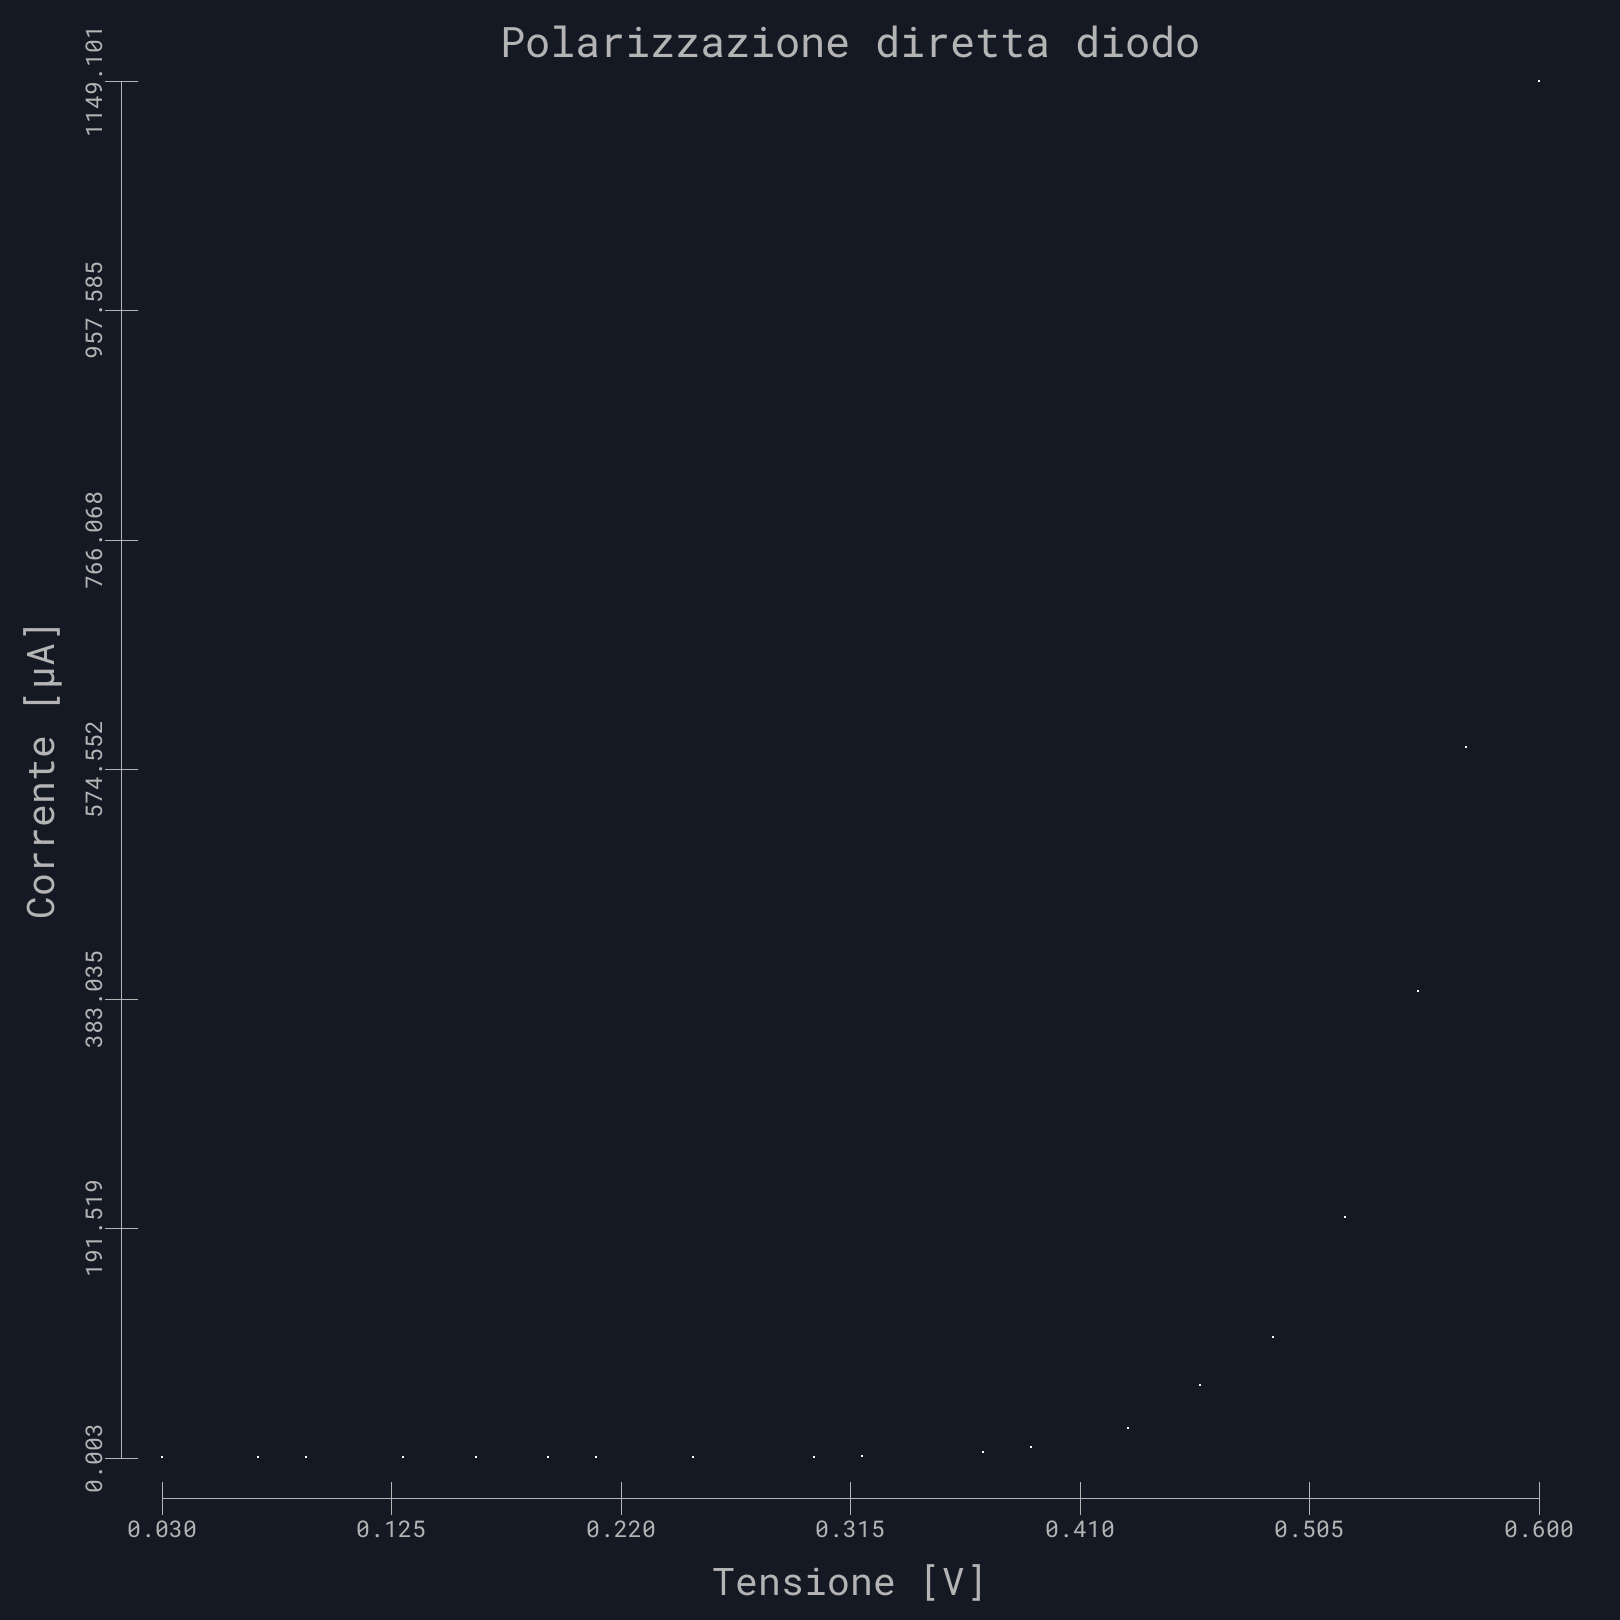
\includegraphics[width=.65\linewidth]{../images/grafico2.png} % Replace example-image with your figure filename
    \caption{Corrente in polarizzazione diretta}
    \label{grafico:2}
\end{figure}

\newpage

\begin{figure}[h]
    \begin{minipage}{0.5\textwidth} % Adjust the width as needed
        \paragraph{Polarizzazione diretta:}
        Non conoscendo l'orientazione del diodo a priori, abbiamo intuito quale fosse il verso della polarizzazione dall'andamento della curva caratteristica corrente-tensione. Abbiamo realizzato il circuito come in Figura \ref{circuito:2}; abbiamo impostato la configurazione dell'alimentatore per la misura in forward bias: dato che la I ha crescita esponenziale, abbiamo dovuto settare piccole variazioni di tensione per non avere valori troppo grandi di corrente e riuscire ad analizzare l'andamento prima di raggiungere il plateau. Abbiamo registrato i valori di corrente in funzione della tensione applicata, i dati sono riportati nella tabella \ref{tab:tabella2}. Abbiamo usato un'errore strumentale basandoci sull'ultima cifra stabile misurata.
    \end{minipage}
    \hfill % Add horizontal space between minipages
    \begin{minipage}{0.4\textwidth} % Adjust the width as needed
        \centering
        \includegraphics[width=\linewidth]{../images/circuito2.png} % Replace example-image with your figure filename
        \caption{circuito per caratterizzazione di un LED forward}
        \label{circuito:2}
    \end{minipage}
\end{figure}

\begin{figure}[h]
    \begin{minipage}{0.5\textwidth} % Adjust the width as needed
        \paragraph{Polarizzazione inversa:}
        Abbiamo realizzato il circuito come in Figura \ref{circuito:3}. Abbiamo impostato la configurazione dell'alimentatore per la misura in reverse bias e abbiamo registrato la corrente in funzione della tensione applicata leggendo i valori di V direttamente dal generatore: 
        \newline
        se avessimo messo in parallelo al diodo il voltmetro (come nella misura precedente), la grossa differenza di R (molto più grande nel diodo) avrebbe portato alla sola caratterizzazione della resistenza interna del voltmetro, e non del diodo.
        \newline
        \newline
        Riportiamo la tabella \ref{tab:tabella4} con i dati in appendice e la Figura \ref{grafico:4} delle misure nel paragrafo dell'analisi dati, insieme al fit.
    \end{minipage}
    \hfill % Add horizontal space between minipages
    \begin{minipage}{0.4\textwidth} % Adjust the width as needed
        \centering
        \includegraphics[width=\linewidth]{../images/circuito3.png} % Replace example-image with your figure filename
        \caption{circuito per caratterizzazione di un LED inverso}
        \label{circuito:3}
    \end{minipage}
\end{figure}

\newpage

\subsubsection{Analisi dati}

\paragraph{Polarizzazione diretta:}

Abbiamo effettuato un fit lineare dei dati precedenti in scala logaritmica con la funzione interpolante $y=ax+b$, e abbiamo sfruttato la relazione: 
$$I=I_0 \left[\exp\left(\frac{qV}{\eta k_B T}\right)-1\right]$$ 
\newline
sapendo che in polarizzazione diretta:

$$V>\frac{\eta k_B T}{q} \quad \therefore \quad I \sim I_0 \left[\exp\left(\frac{qV}{\eta k_B T}\right) \right]$$
\newline
Applicando il logaritmo abbiamo potuto eguagliare la pendenza:

$$a = \frac{q}{\eta k_B T} \quad \therefore \quad \eta = \frac{q}{ak_B T}$$
\newline
Inoltre, dall'intercetta $b=ln(I_0)$ abbiamo ricavato $I_0=e^b$.
\newline
\newline
Riportiamo in tabella \ref{tab:tabella2} i dati della tensione in funzione della corrente e del $\ln(I)$.
\\
In Figura \ref{grafico:3} è riportato l'andamento dei dati con i relativi errori (gli errori della prima metà del grafico sono di 5 ordini di grandezza più piccoli rispetto alla scala delle Y, dunque non sono visualizzabili sullo schermo). Il $\chi^2$ estremamente diverso da 1 indica un grave errore nell'ordine di grandezza degli errori delle misure. Infatti $\chi^2$ molto grandi sono indice di errori troppo piccoli per fittare correttamente i dati.
\begin{figure}[h]
    \begin{minipage}{0.69\textwidth} % Adjust the width as needed
        \centering
        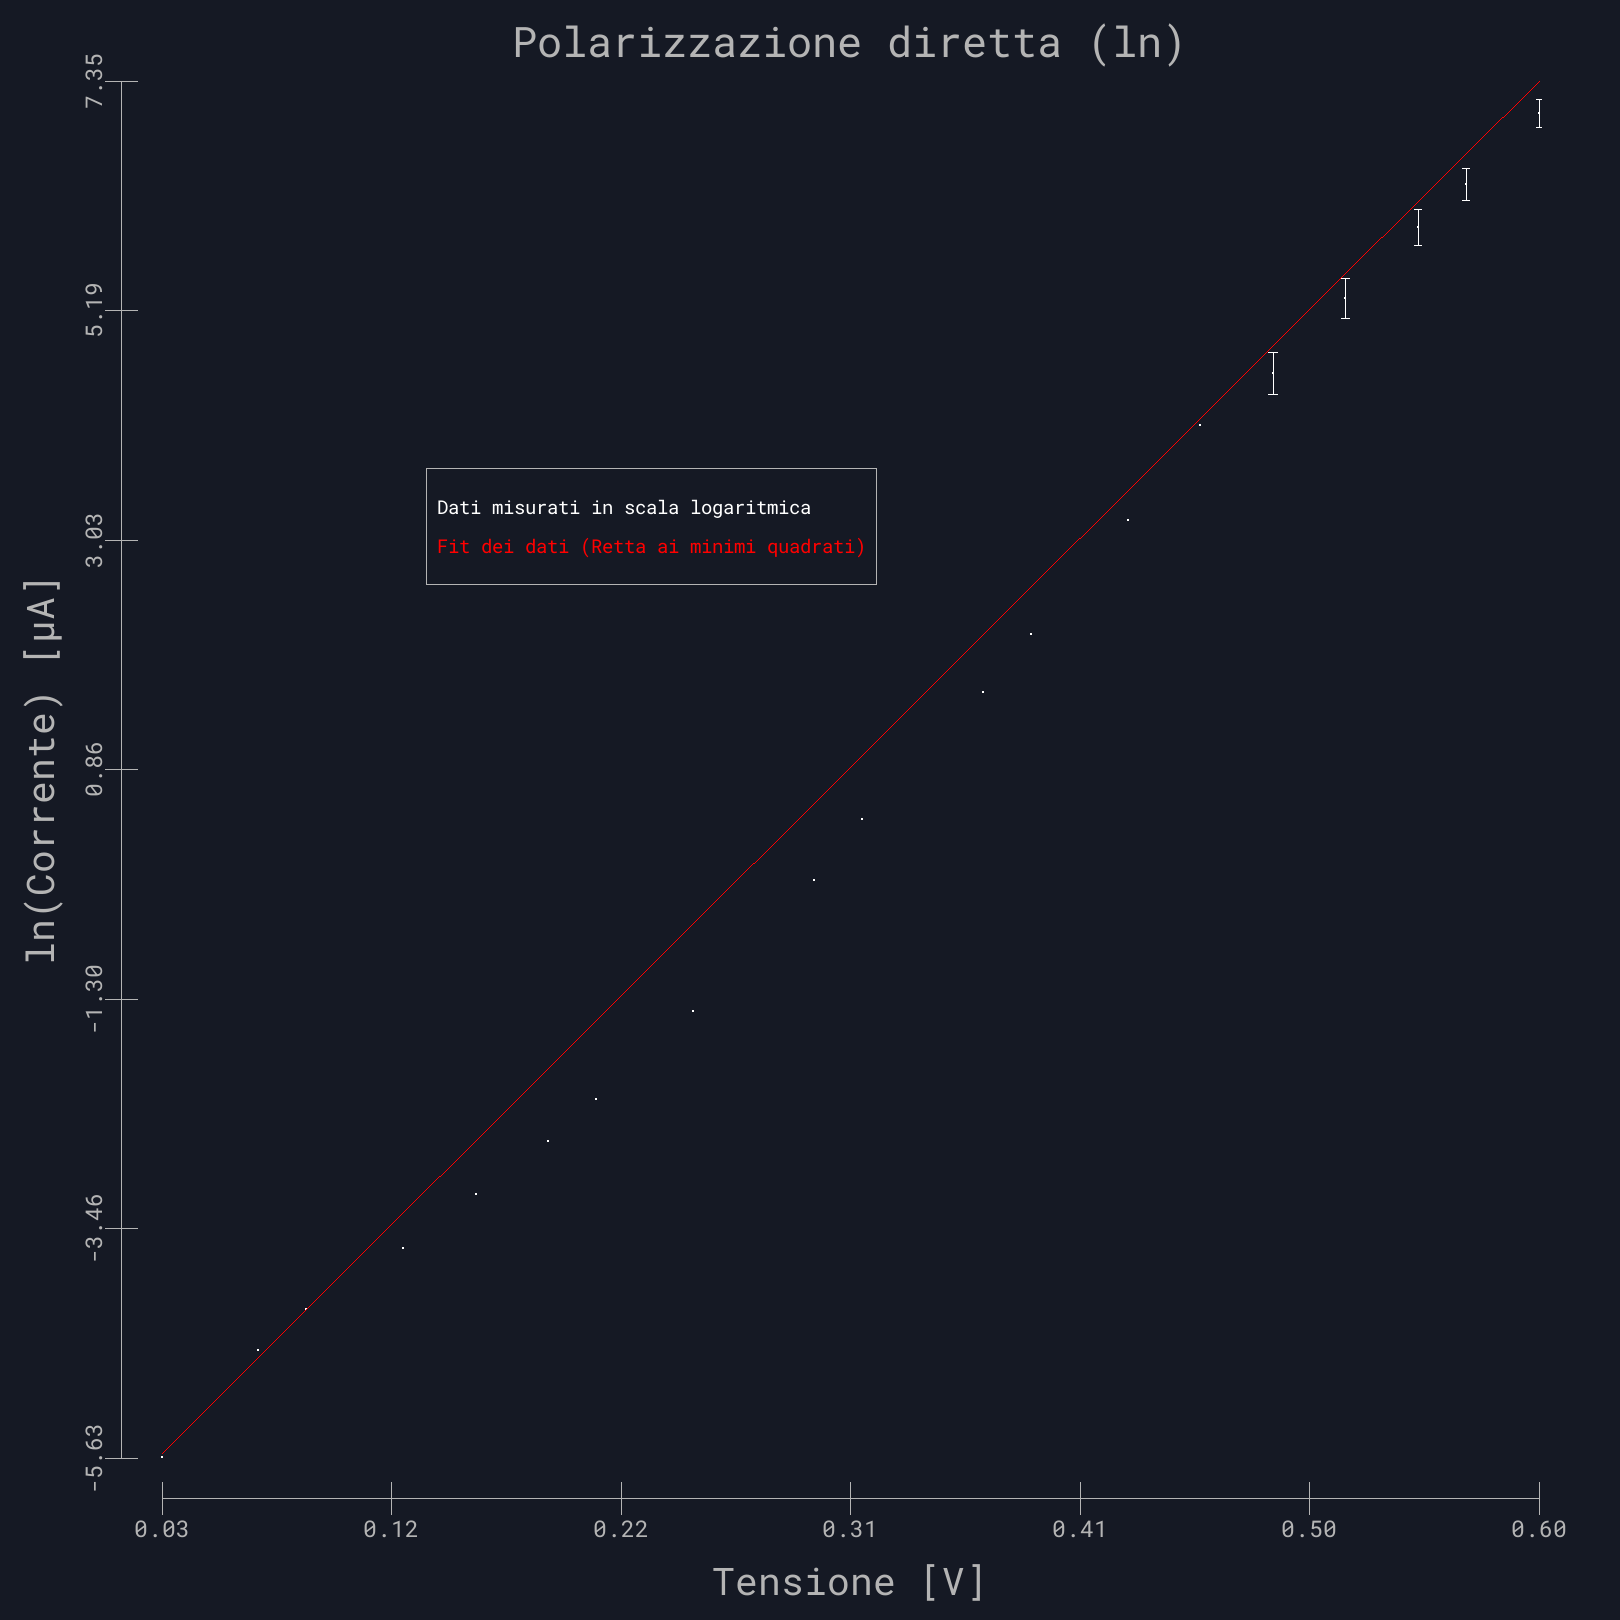
\includegraphics[width=1\linewidth]{../images/grafico3.png} % Replace example-image with your figure filename
        \caption{Polarizzazione diretta di un diodo riportato in base logaritmica}
        \label{grafico:3}
    \end{minipage}
    \hfill % Add horizontal space between minipages
    \begin{minipage}{0.3\textwidth}    
    \begin{itemize}
        \item Considerando $\frac{k_BT}{q} = 0.026V$
        \item $a=(22.39 \pm 0.19 )V^{-1}$
        \item $b=(-6.37 \pm 0.08)\mu A$
        \item $\chi^2 = 75138.68$
        \item $\eta=1.718 \pm 0.015$
        \item $I_0= (0.00171 \pm 0.00014) \mu A = (1.71 \pm 0.14) nA$
    \end{itemize}
    \end{minipage}
\end{figure}

\newpage

\paragraph{Polarizzazione inversa:}
Abbiamo fatto un fit con l'equazione $y=ax+b$ della sola parte lineare. Dato che abbiamo registrato piccolissime variazioni di corrente, e dato che il generatore, per poter erogare diversi range di corrente possiede anch'esso una piccola resistenza (che in genere non inficia sui dati ma nel nostro caso l'ha fatto dato l'ordine di grandezza di $I$) abbiamo notato uno scalino che interrompe la linearità della curva caratteristica, per cui abbiamo deciso di troncarla per poter fare il fit. I dati sono riportati in tabella \ref{tab:tabella4}. Tenendo conto del contributo della resistenza interna al diodo (resistenza di Shant), possiamo scrivere che la caratteristica corrente/tensione per tensioni in polarizzazione inversa sufficientemente elevate assume l'espressione:

$$I=-I_0+\left(\frac{V}{R_{Sh}} \right)$$ 

per cui la pendenza $a$ del fit è uguale a $1/R_{Sh}$ ,  mentre $-I_0=b$.

\begin{figure}[h]
    \begin{minipage}{0.59\textwidth} % Adjust the width as needed
        \centering
        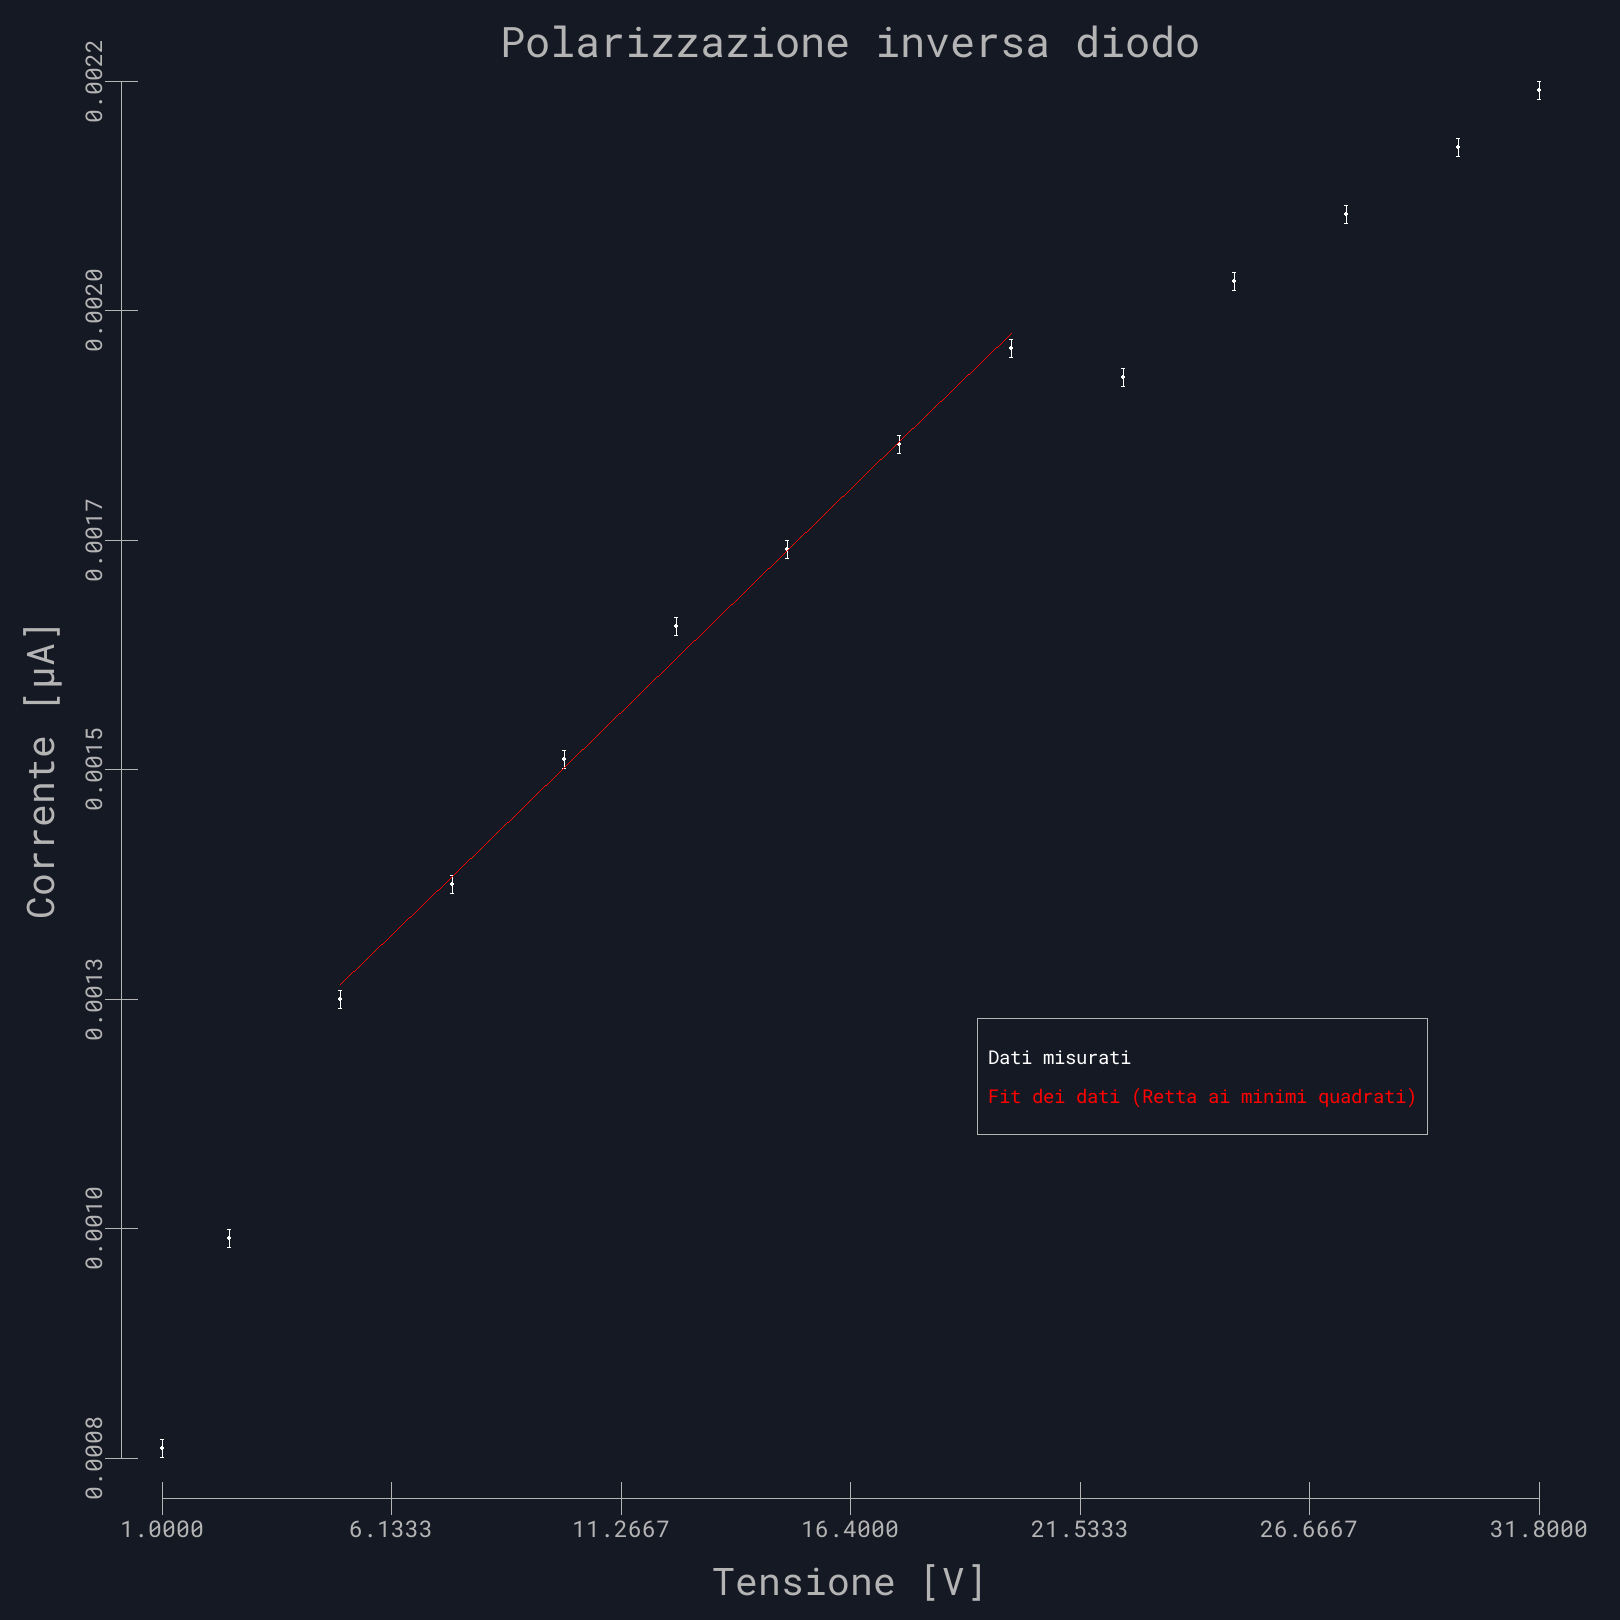
\includegraphics[width=1\linewidth]{../images/grafico4.png} % Replace example-image with your figure filename
        \caption{Polarizzazione inversa di un diodo}
        \label{grafico:4}
    \end{minipage}
    \hfill % Add horizontal space between minipages
    \begin{minipage}{0.4\textwidth}    
        \begin{itemize}
            \item $a = (0.000040 \pm 0.000003) \mu \Omega^{-1}$
            \item $b = (0.00109 \pm 0.00005) \mu A$
            \item $\chi^2 = 0.28$
            \item Corrente saturazione inversa $= b$
            \item $R_{Sh} = (25.0 \pm 1.9) G\Omega$
        \end{itemize}
    \end{minipage}
\end{figure}

\subsubsection{Propagazione degli errori ($\sigma$): }

\paragraph{Polarizzazione diretta:} 
$$\sigma_{\eta}=\eta*\sigma_a/a$$
$$\sigma_{I_0}=\sigma_b*e^b$$
\paragraph{Polarizzazione inversa:}
$$\sigma_{R_{Sh}}=R_{Sh}\frac{\sigma_a}{a}$$

\subsubsection{Conclusioni}

Tramite queste misurazioni abbiamo potuto verificare che l'andamento della tensione in funzione della corrente all'interno di un diodo è abbastanza coerente con quello che ci aspettavamo.

\subsection{Caratterizzazione di diodi emettitori di luce (LED)}
\subsubsection{Scopo dell'esperienza}
In questa esperienza abbiamo caratterizzato un led servendoci di uno spettrometro e dei multimetri usati nell'esperienza 1.1. Così facendo, abbiamo potuto determinare la lunghezza d'onda di emissione del led, il fattore d'idealità, la corrente di saturazione inversa, la tensione di turn on e la corrente di turn on.

\subsubsection{Strumentazione}
\begin{itemize}
    \item Voltmetro AMPROBE 37XR-A
    \item Generatore di tensione GWINSTEK GPS-4303
    \item Amperometro RSPRO IDM 103N
    \item Universal Breadboard
    \item Cablaggio
    \item LED che emette nell'arancione
    \item resistenza da $(1 \pm 0.5) k\Omega$ 
    \item Spettrometro Ocean Optics (S13335) 
    \item PC con software SpectraSuite    
    \item sensibilità voltmetro: $\pm0.1\% + 5 dgts$
    \item sensibilità amperometro: $\pm0.6\%+2 dgts$
\end{itemize}

\subsubsection{Procedimento}

\begin{figure}[h]
    \begin{minipage}{0.7\textwidth} % Adjust the width as needed
        Abbiamo realizzato il circuito come in Figura \ref{circuito:4}. Abbiamo poi posizionato il diodo in direzione dello spettrometro collegato al pc. Dopo aver acquisito il segnale di buio per il background, abbiamo cominciato a misurare per diversi valori di tensione $V_{in}$  del generatore, la $V$ dal voltmetro, la corrente dall'amperometro e l'intensità luminosa del led (integrando il picco tramite il software). Il primo spettro acquisito è stato registrato in modo tale che l'intensità del picco maggiore arrivasse quasi a saturazione. Ne abbiamo riportato la lunghezza d'onda e la FWHM (tempo di integrazione: 1s, medie di misurazioni usate: 1):
        \begin{itemize}
            \item $\lambda=(623\pm18)  nm$
            \item FWHM $=36  nm$
            \item energia $E=  (1.99\pm0.06 )eV$
        \end{itemize}
    \end{minipage}
    \hfill % Add horizontal space between minipages
    \begin{minipage}{0.25\textwidth} % Adjust the width as needed
        \centering
        \includegraphics[width=\linewidth]{../images/circuito2.png} % Replace example-image with your figure filename
        \caption{circuito per caratterizzazione di un LED}
        \label{circuito:4}
    \end{minipage}
\end{figure}

Abbiamo riportato solo 6 picchi per non sovraffollare la Figura \ref{grafico:9/10}a, e perché a bassi valori di corrente l'amperometro non era in grado di registare dei dati stabili.
Abbiamo effettuato una caratteristica tensione-corrente: a causa della scarsa precisione degli strumenti usati, non abbiamo potuto registrare i dati nel range interessato, cioè per valori di corrente piccoli, per cui nella Figura \ref{grafico9} la zona iniziale di plateau non è visibile, mentre è visibile il secondo plateau a più alte correnti. Per questo motivo i risultati da noi ottenuti non sono accurati. Riportiamo i dati nella tabella \ref{tab:tabella5} e nella Figura \ref{grafico:9/10}b.

\begin{center}
    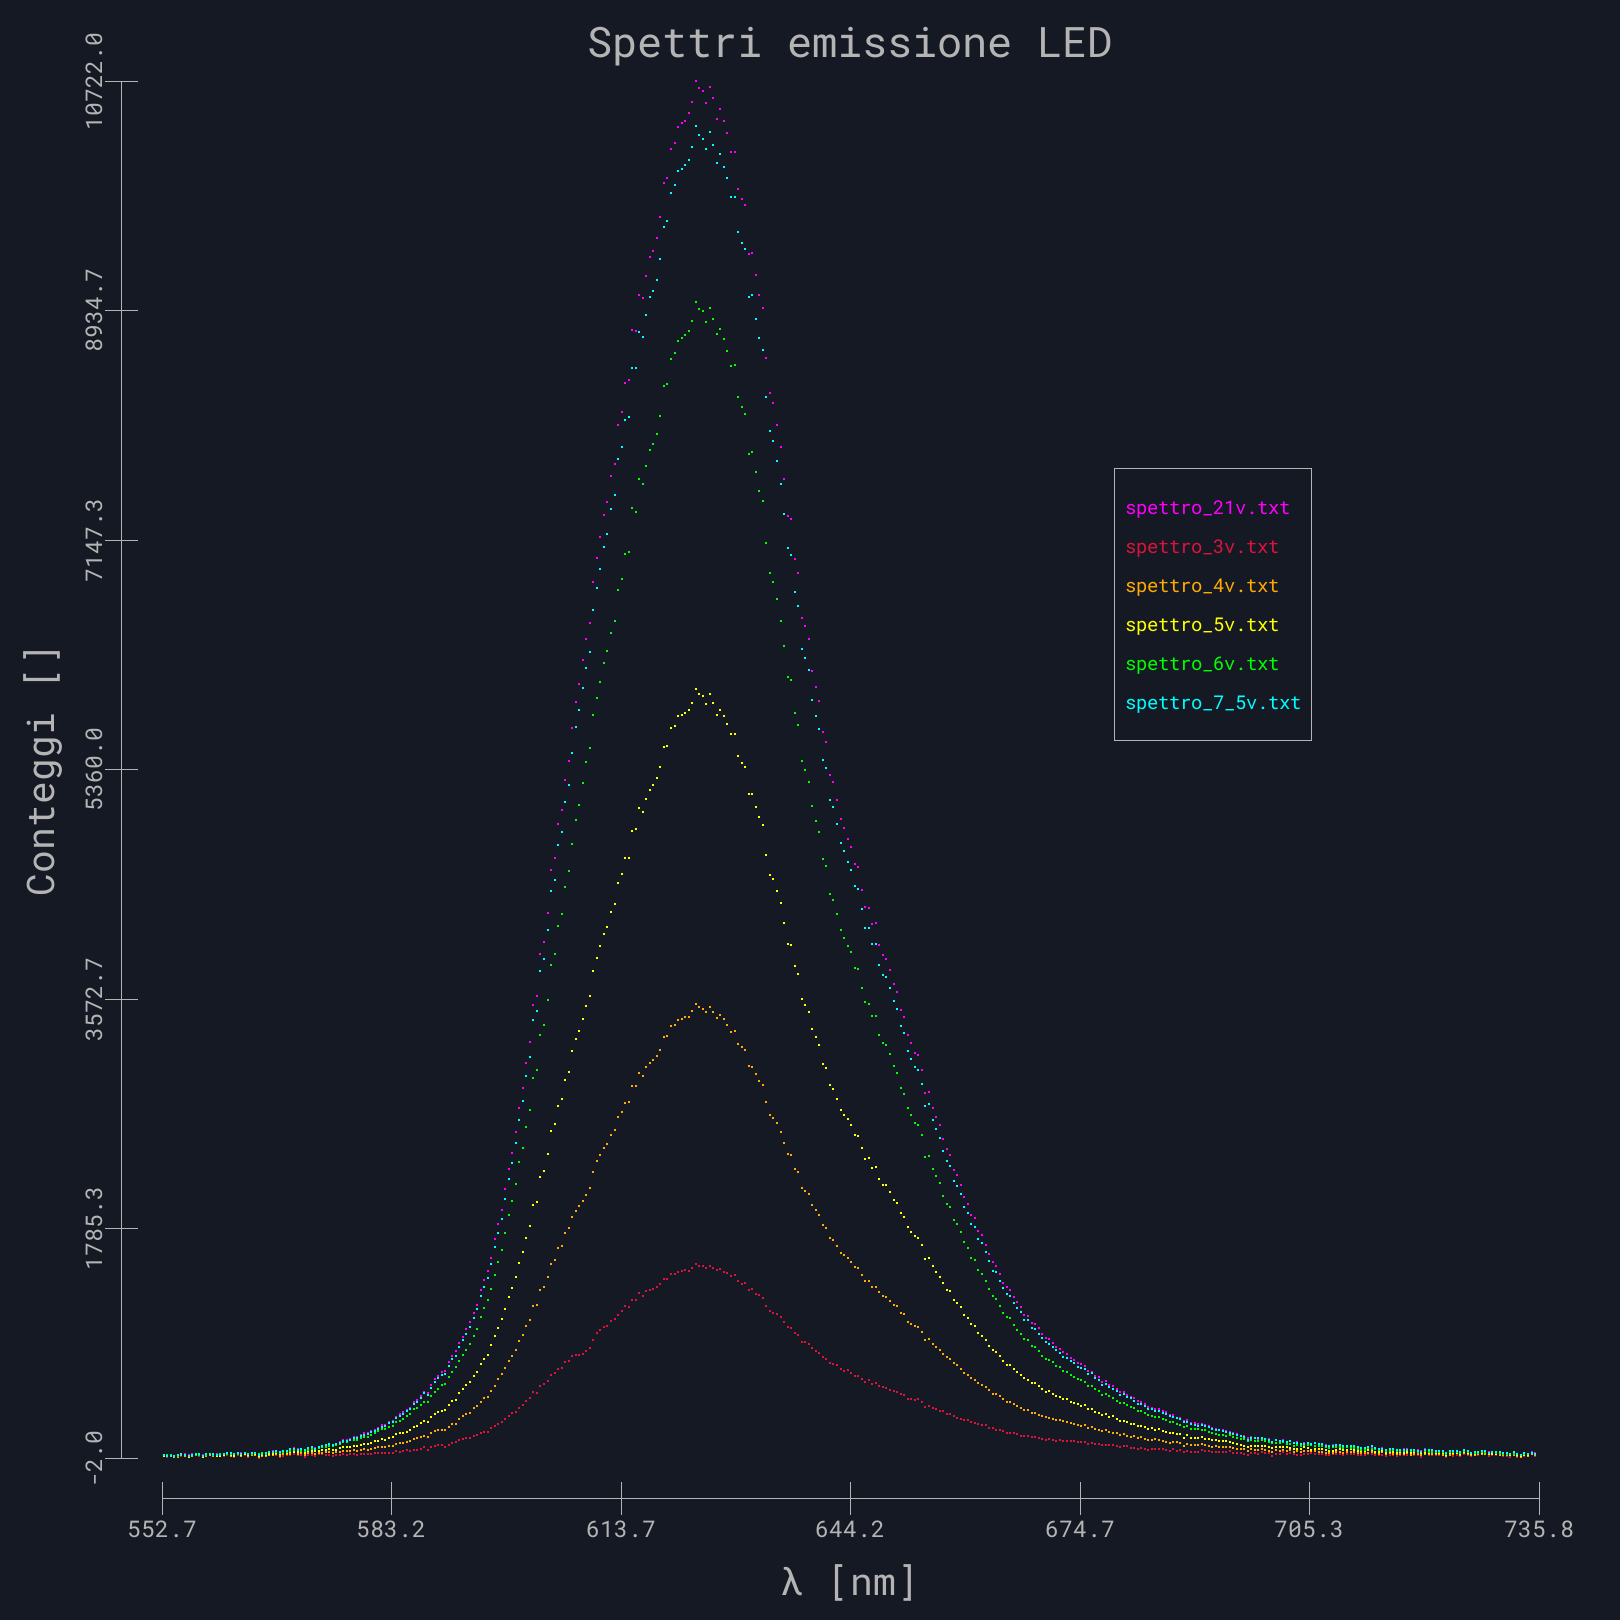
\includegraphics[width=.45\textwidth]{../images/grafico5.png}
    \hfill
    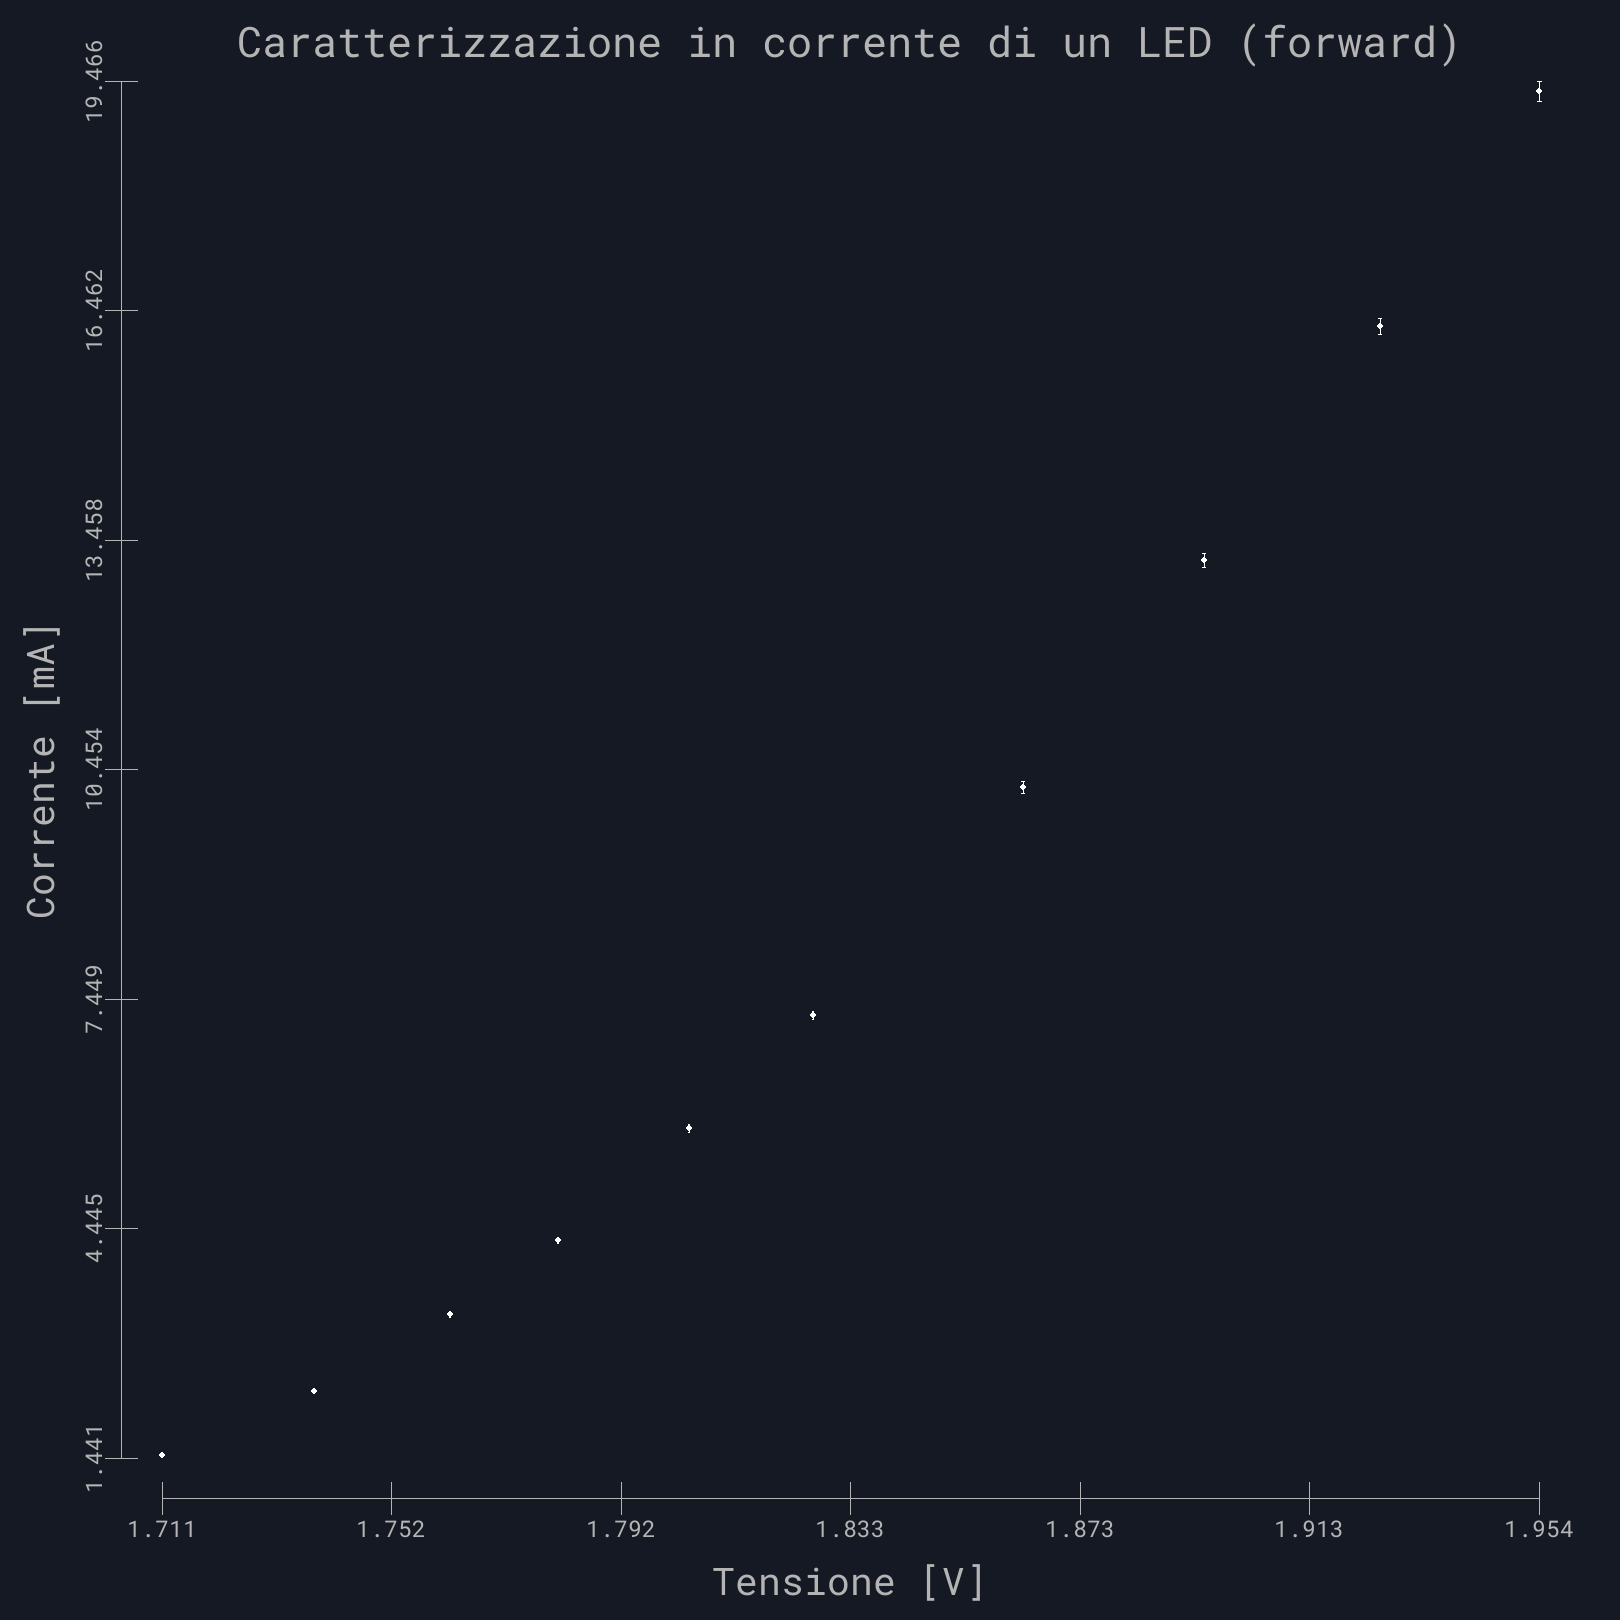
\includegraphics[width=.45\textwidth]{../images/grafico6.png}
    \captionof{figure}{a) Spettri di emissione a varie tensioni, b) Caratteristica corrente-tensione in scala lineare (tensione misurata sul diodo)}
    \label{grafico:9/10}
\end{center}

\subsubsection{Analisi dati}
Abbiamo effettuato un fit lineare dei dati precedenti in scala logaritmica con la funzione interpolante $y=ax+b$, e abbiamo sfruttato la relazione: 
$$I=I_0 \left[\exp\left(\frac{qV}{\eta k_B T}\right)-1\right]$$ 
\newline
sapendo che in polarizzazione diretta:

$$V>\frac{\eta k_B T}{q} \quad \therefore \quad I \sim I_0 \left[\exp\left(\frac{qV}{\eta k_B T}\right) \right]$$
\newline
Applicando il logaritmo abbiamo potuto eguagliare la pendenza:

$$a = \frac{q}{\eta k_B T} \quad \therefore \quad \eta = \frac{q}{ak_B T}$$
\newline
Inoltre, dall'intercetta $b=ln(I_0)$ abbiamo ricavato $I_0=e^b$.
\begin{center}
    \begin{minipage}{.6\textwidth} % Adjust the width as needed
        \centering
        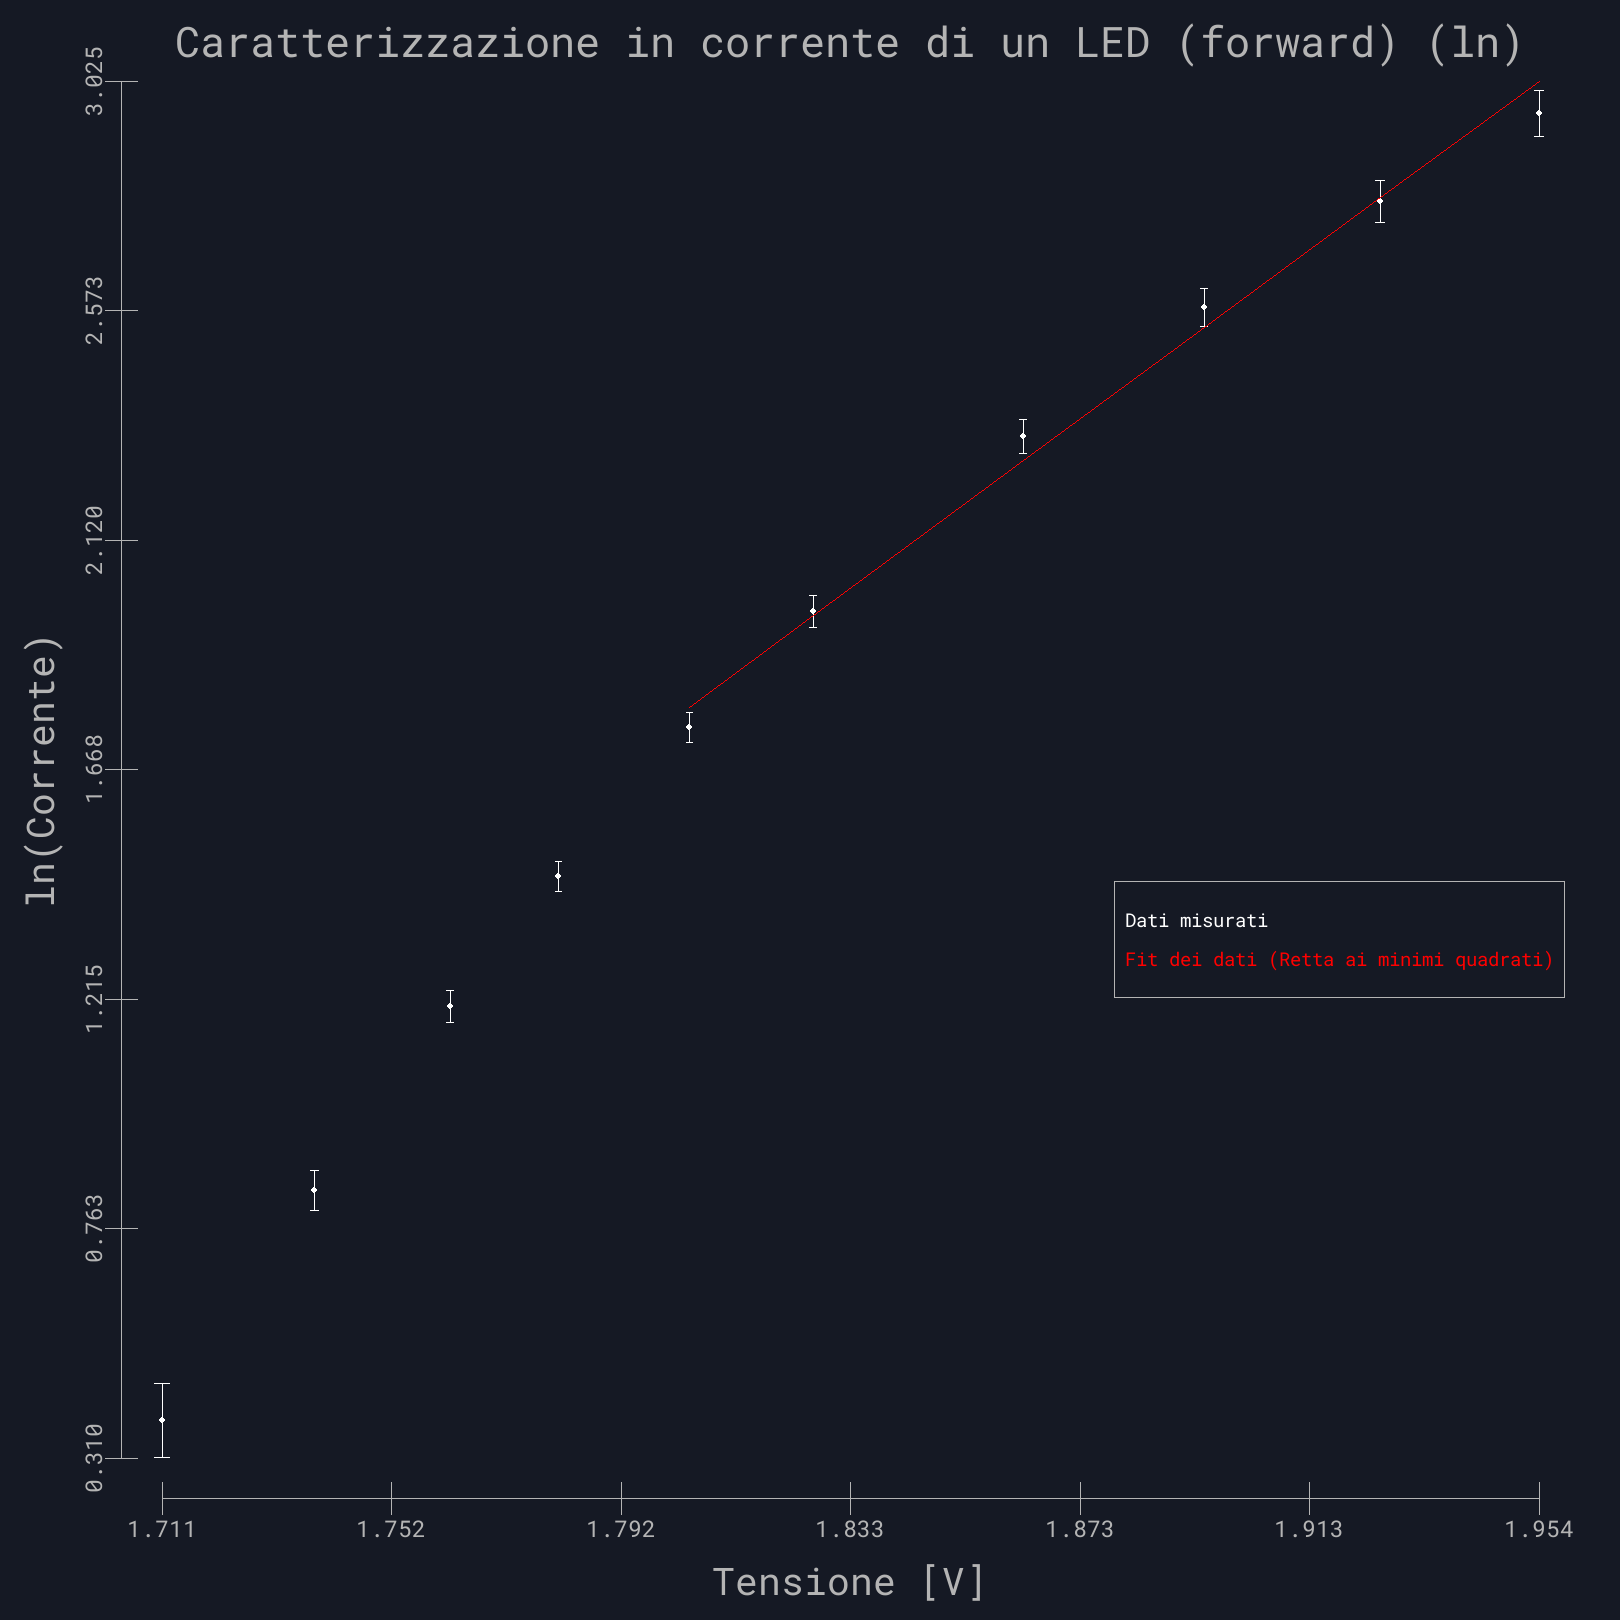
\includegraphics[width=\linewidth]{../images/grafico7.png} % Replace example-image with your figure filename
        \captionof{figure}{Caratteristica corrente-tensione (del diodo) in scala ln}
        \label{grafico7}
    \end{minipage}
    \hfill
    \begin{minipage}{0.35\textwidth} % Adjust the width as needed
        \paragraph{FIT1}
        \begin{itemize}
            \item $a=( 7.8\pm0.3 ) V^{-1}$ 
            \item $b=(-12.2 \pm 0.6)mA $
            \item $\chi^2=0.77$
            \item $I_0=(5*10^{-6}  \pm3*10^{-6}  )mA=(5\pm3)nA$
            \item $\eta=( 4.93\pm0.19)$
            \item Range di interpolazione: da $1.804 V$ a $1.954V$
        \end{itemize}
    \end{minipage}
    \hfill % Add horizontal space between minipages
\end{center}

Tramite il fit della tensione di entrata in funzione della corrente invece abbiamo potuto estrapolare la tensione di Turn-On, ottenuta tramite l'intersezione con l'asse $X$.

\begin{center}
    \begin{minipage}{.6\textwidth} % Adjust the width as needed
        \centering
        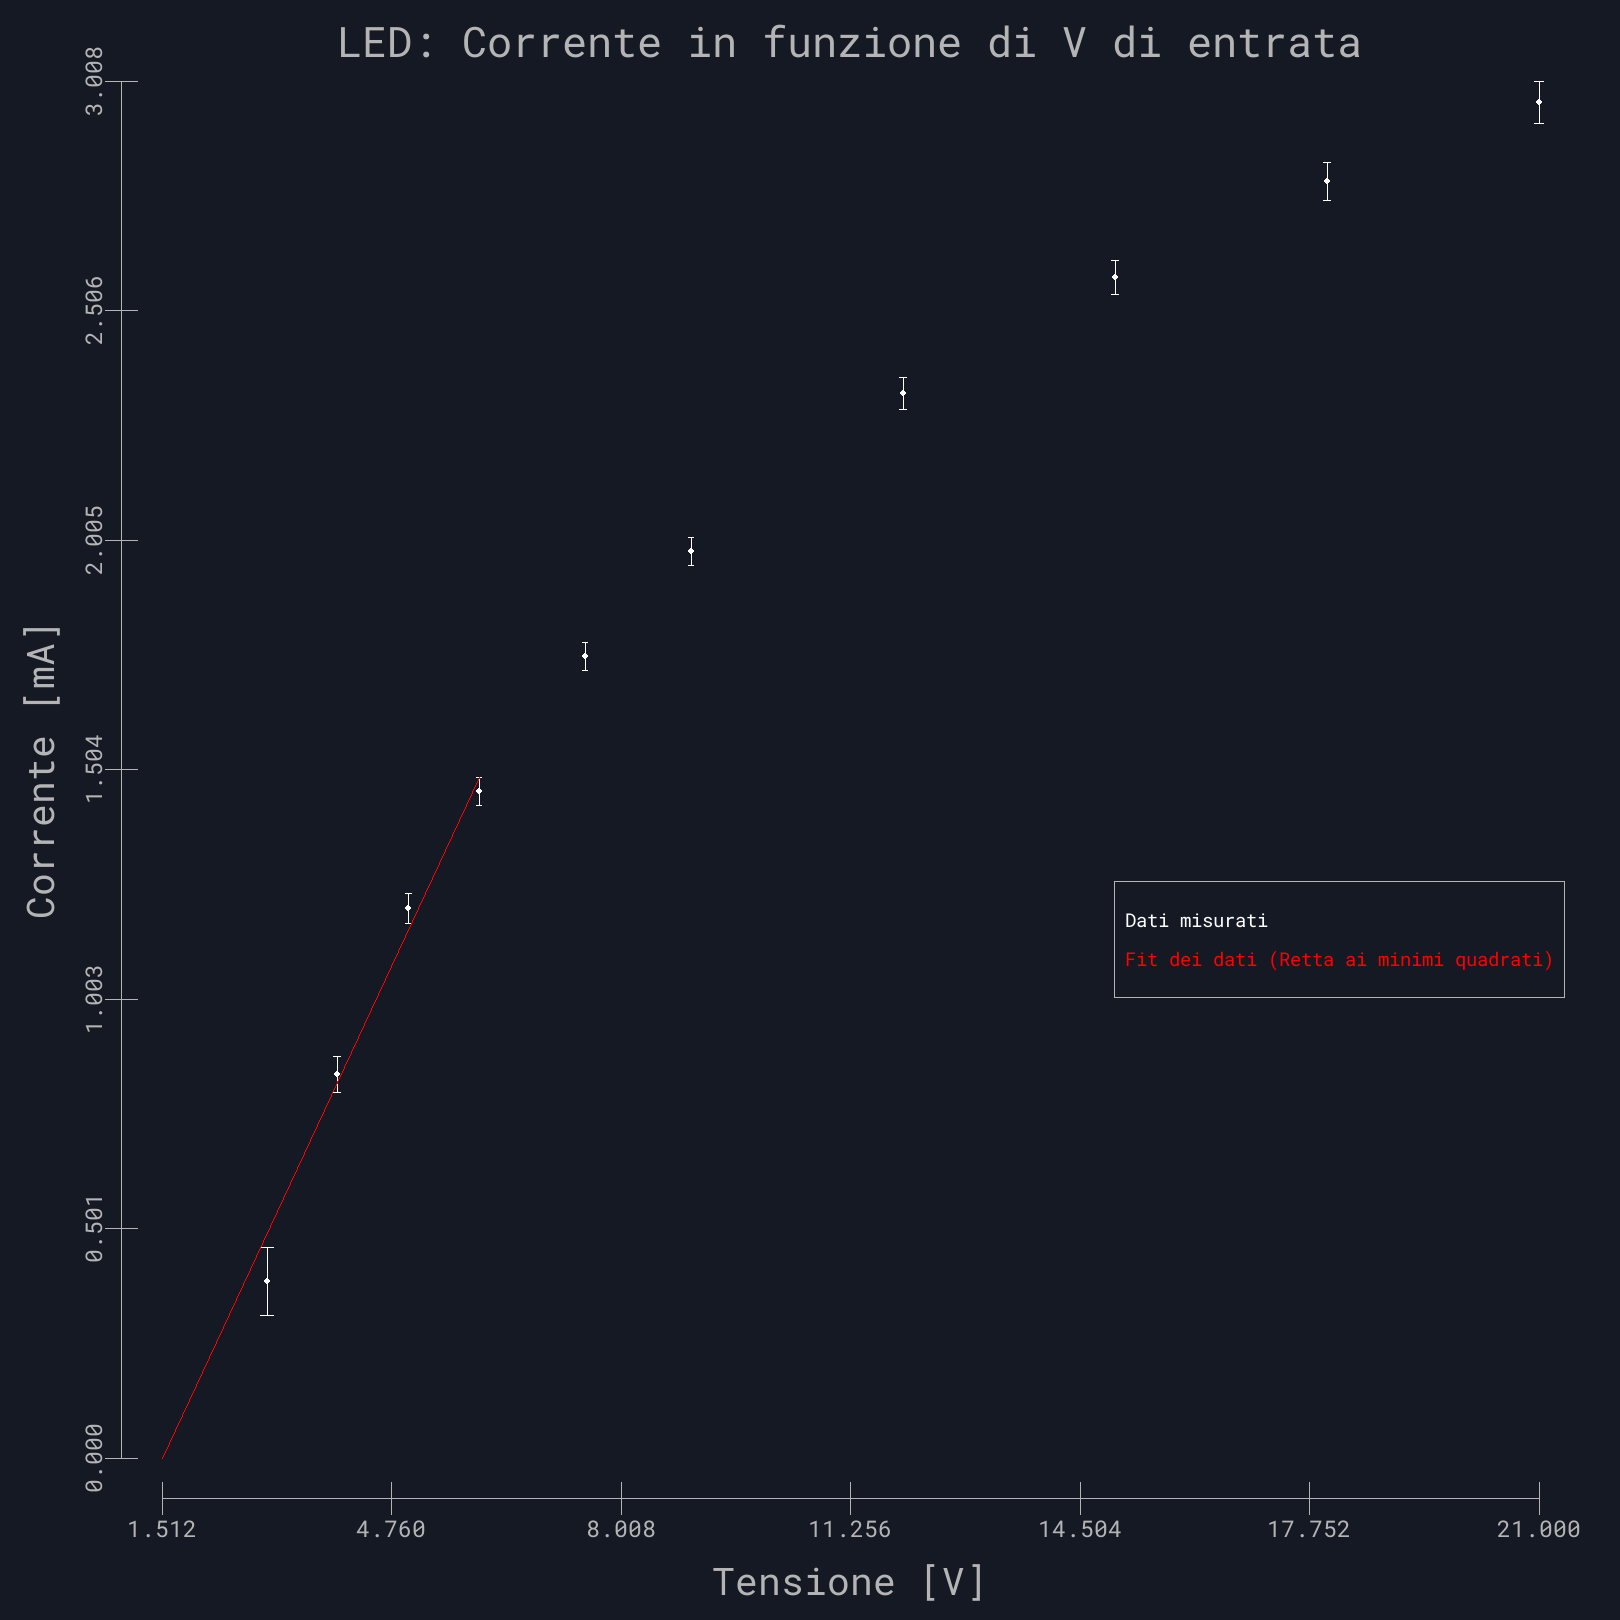
\includegraphics[width=\linewidth]{../images/grafico8.png} % Replace example-image with your figure filename
        \captionof{figure}{Dati caratterizzazione LED (2)}
        \label{grafico8}
    \end{minipage}
    \hfill
    \begin{minipage}{0.35\textwidth} % Adjust the width as needed
        \paragraph{FIT2}
        \begin{itemize}
            \item $a=( 0.33\pm0.03 ) V^{-1}$
            \item $b=(-0.50\pm 0.17)mA $
            \item $\chi^2=2.45$
            \item $V_{TO}=(1.5\pm0.7 )V $
            \item Range di interpolazione: da $3 V$ a $6 V$
        \end{itemize}
    \end{minipage}
    \hfill % Add horizontal space between minipages
\end{center}

Infine, tramite il fit della parte lineare della corrente in funzione dell'intensità luminosa abbiamo potuto estrapolare la corrente di Turn-On leggendola sull'intersezione dell'asse $X$.

\begin{center}
    \begin{minipage}{.6\textwidth} % Adjust the width as needed
        \centering
        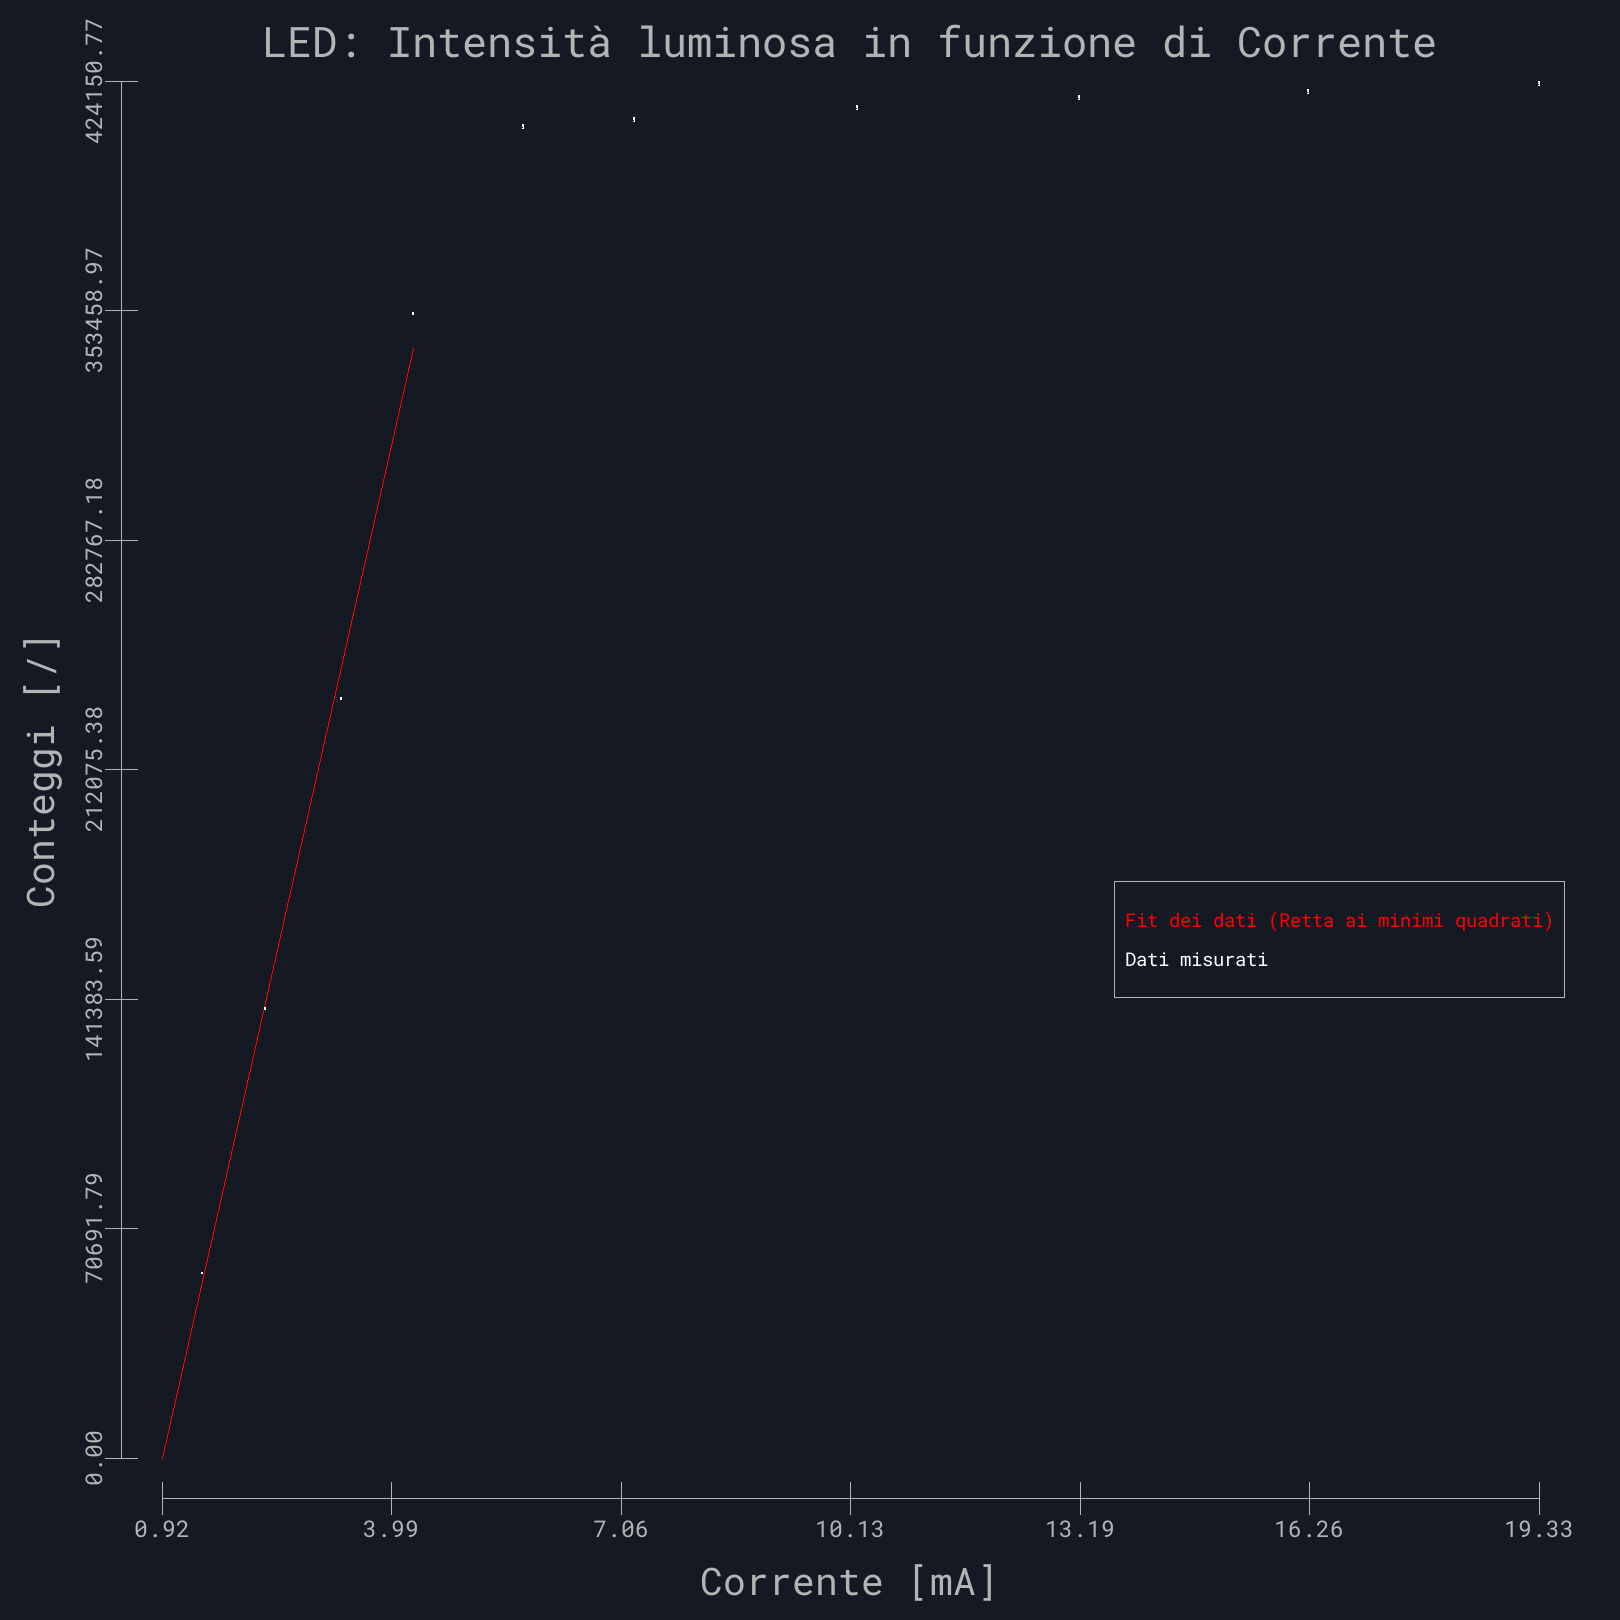
\includegraphics[width=\linewidth]{../images/grafico9.png} % Replace example-image with your figure filename
        \captionof{figure}{Dati caratterizzazione LED (3)}
        \label{grafico9}
    \end{minipage}
    \hfill
    \begin{minipage}{0.35\textwidth} % Adjust the width as needed
        \paragraph{FIT3}
        \begin{itemize}
            \item $a=( 1.02*10^{5}\pm4 * 10^3 )mA^{-1}$
            \item $b=(-9.4*10^4\pm 9*10^3)  $
            \item $\chi^2=380$
            \item $I_{TO}=(0.93\pm0.05 )mA$
            \item Range di interpolazione: da $1.47 mA$ a $4.29 mA$
        \end{itemize}
    \end{minipage}
    \hfill % Add horizontal space between minipages
\end{center}


\subsubsection{Propagazione degli errori ($\sigma$): }

$$\sigma_E=E\frac{\sigma_{\lambda}}{\lambda} \sim 0.06 eV$$
Fit 1:
$$\sigma_{\eta}=\eta\frac{\sigma_a}{a}\sim 0.19$$
$$\sigma_{I_0}=\sigma_be^b \sim 3*10^{-6} mA$$
Fit 2:
$$V_{TO}=-\frac{b}{a}$$
$$\sigma_{V_{TO}}=V_{TO}\left(\frac{\sigma_a}{a}+\frac{\sigma_b}{b}\right)\sim0.7V$$
Fit  3:
$$I_{TO}=-\frac{b}{a}$$
$$\sigma_{I_{TO}} = I_{TO}\left(\frac{\sigma_a}{a}+\frac{\sigma_b}{b}\right)\sim0.05 mA$$


\subsubsection{Conclusioni}
I risultati sono coerenti con quello che ci aspettavamo (nonostante il $\chi^2$ fortemente maggiore di 1, il che indica che gli errori sono molto più piccoli della dispersione statistica dei dati raccolti), confermano inoltre ciò che potevamo vedere empiricamnente, infatti il led era di colore arancione e la lunghezza d'onda rilevata è di 623 nm.

\newpage
\section{Fotoconducibilità}

\subsection{Scopo dell'esperienza}

\subsection{Strumentazione}
\begin{itemize}
    \item Spettrometro USB 4000
    \item Lampada calibrata  HG-2 (Hg-Ar)
    \item Pc con software ocean optics Spectrasuite
    \item Fibra ottica
    \item Oscilloscopio Tektronix  TBS1104
    \item Monocromatore MINI-CHROM 1
    \item Chopper a 80 Hz
    \item Generatore di tensione GWinstek GPS-4303 (24.8V)
    \item Fotodiodo al silicio DET-100-A2 biased detector 320-1100 nm
    \item Campione semiconduttore su supporto e resistenza
    \item Lampada alogena 
    \item Supporti meccanici per la disposizione degli strumenti (breadboard,…)
\end{itemize}

\subsection{Procedimento}
\paragraph{Calibrazione dello spettrometro:}
Abbiamo collegato lo spettrometro al pc e alla lampada con la fibra ottica e abbiamo settato il tipo di scan sul software; Abbiamo registrato due spettri a due tempi d'integrazione diversi (integration time=3,800 $\mu s$ e 14,1 $\mu s$),  e abbiamo impostato gli scans to average a 15. Lo spettro così impostato ha i pixel come grandezza sull'asse delle x e i conteggi sulle y; abbiamo allentato leggermente la vite della fibra ottica allo spettrometro per non avere dei picchi fuori scala nel primo zoom (per rilevare i picchi abbiamo ingrandito una volta lo spettro: nel primo “zoom” erano così intensi da dover allentare la fibra ottica, nel secondo l'abbiamo riavvitata).

Abbiamo acquisito il background, poi abbiamo registrato lo spettro per confrontare i picchi in pixel con le lunghezze d'onda teoriche della lampada usata. Per ottenere questa corrispondenza, ci siamo dovuti orientare lungo lo spettro: guardando solo il range del visibile (perché lo spettrometro acquisisce indicativamente nel range del visibile) e guardando le intensità dei picchi rivelati con quelle delle righe spettrali segnate sulla lampada. Di questi picchi abbiamo fatto poi dei fit gaussiani per determinarne i massimi e la FWHM (che corrisponde alla deviazione standard di ogni gaussiana). Abbiamo usato ogni FWHM/2 come errore di ogni picco.
\paragraph{Calibrazione monocromatore:}
Abbiamo collegato tramite fibra ottica il monocromatore allo spettrometro (usando un collimatore tra fibra ottica e monocromatore) e abbiamo orientato la sorgente luminosa al monocromatore interponendo una lente focale condensatrice e il chopper; dopo aver acquisito il dark, abbiamo misurato, per ogni unità arbitraria impostata con la manopola del monocromatore, la lunghezza d'onda del picco (in pixel) sullo spettro acquisito e la FWHM. Con questi dati abbiamo potuto ricavare la retta di calibrazione.
\newline\newline
Tempo d'integrazione: 30 ms. 
\subsubsection{Misure di trasmittanza ottica e di fotocorrente:}
\paragraph{Misura dello spettro di riferimento $(I_0)$:}
Abbiamo montato la sorgente di luce allineata con la lente, il chopper, il monocromatore e il fotodiodo (in quest'ordine). Abbiamo acceso la luce e il chopper e abbiamo posto un panno nero sul monocromatore e il fotodiodo dopo aver collegato il fotodiodo all'oscilloscopio (Channel 1) e un amplificatore in serie. Sull'oscilloscopio abbiamo impostato la suddivisione della griglia (5 mV) per un tempo di 2.5 ms. Abbiamo registrato per diverse lunghezze d'onda (e quindi diverse unità arbitrarie impostate dal monocromatore) le ampiezze del segnale dell'oscilloscopio. 
Questi dati sono serviti per poi normalizzare i dati della misura successiva, considerando una sensibilità dell'oscilloscopio pari a $\pm0.40 mV$, che è stata presa in base al rumore elettrico di fondo riportato sullo strumento.  
\paragraph{Misura di trasmittanza e fotocorrente:}
Abbiamo posizionato il campione tra il fotodiodo e il monocromatore. Abbiamo polarizzato il campione collegandolo ad un generatore di tensione impostando una tensione di 24.8 V. Il set up sperimentale è come nella seguente figura:

\begin{center}
    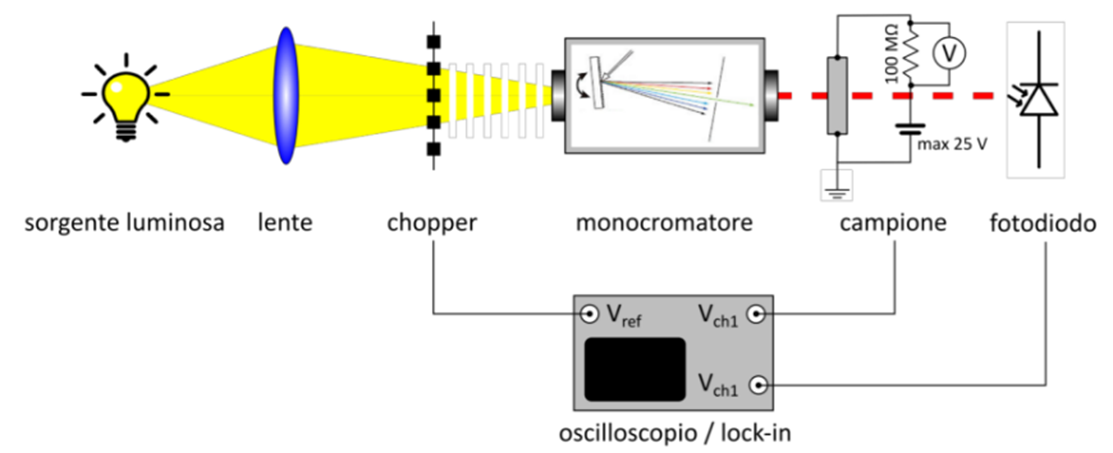
\includegraphics[width=.45\textwidth]{../images/circuito4.png}
    \hfill
    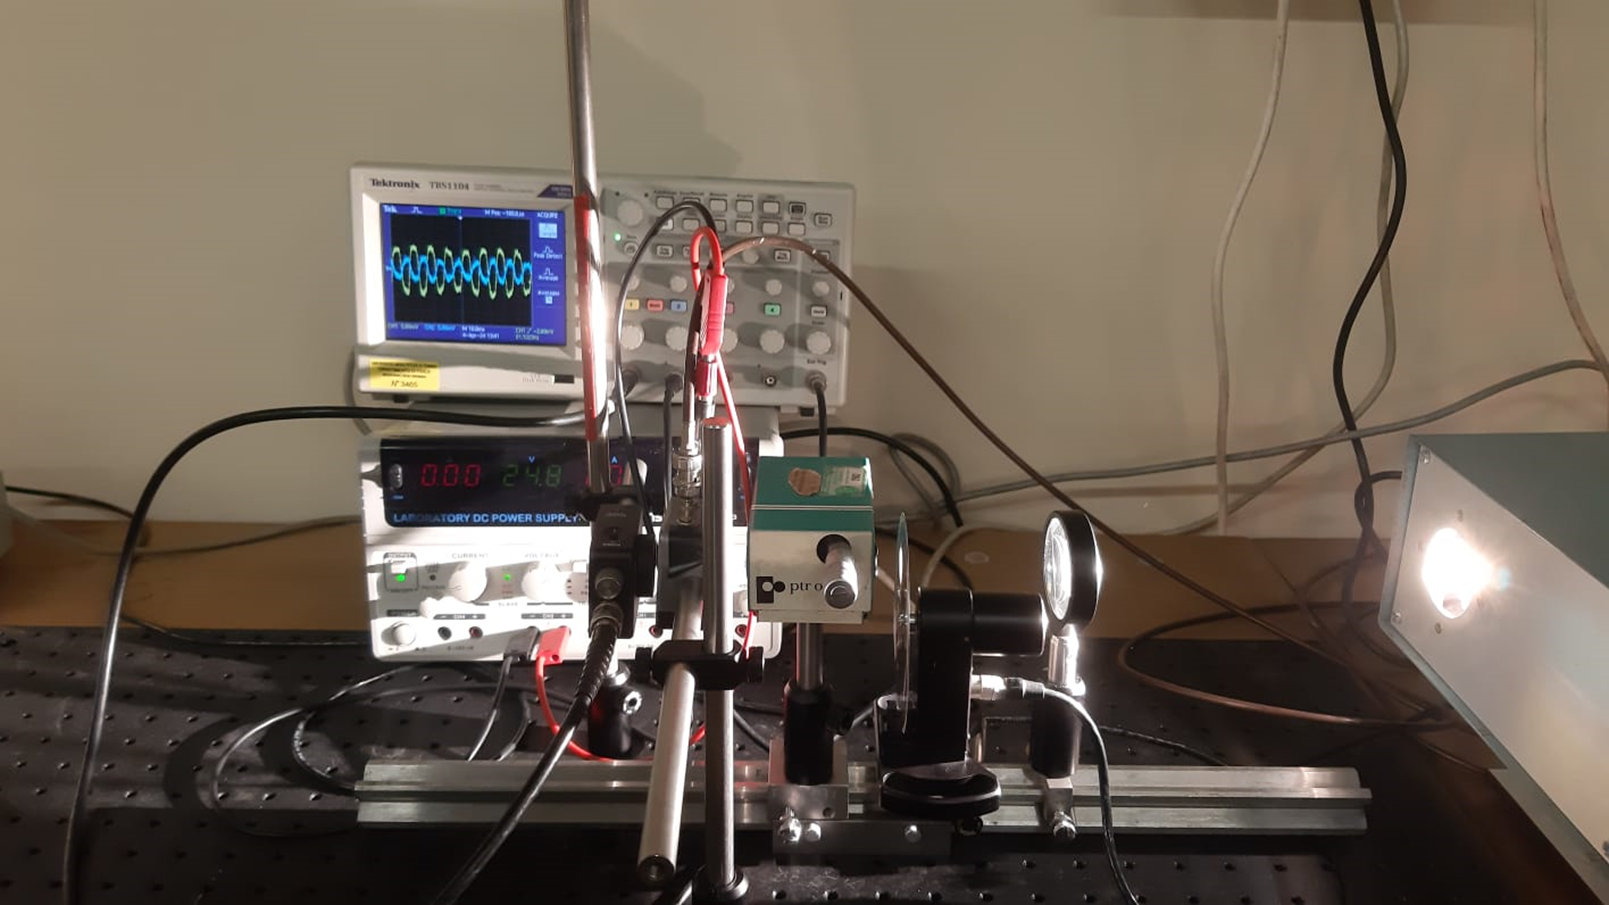
\includegraphics[width=.45\textwidth]{../images/circuito5.png}
    \label{fig:led_circuito}
\end{center}

Come in figura, il canale 2 dell'oscilloscopio è stato collegato al campione polarizzato. Abbiamo poi messo un panno scuro sul monocromatore, il campione e il fotodiodo, e sono state così prese le misure di fotocorrente (lette dalle tensioni del canale 2) e di intensità trasmessa (lette dalle tensioni del canale 1).   
\\
Nei grafici l'asse X misura le lughezze d'onda $\lambda$, e non in unità arbitraria. Questo perchè la conversione è già stata fatta usando le calibrazioni precedenti.

\begin{center}
    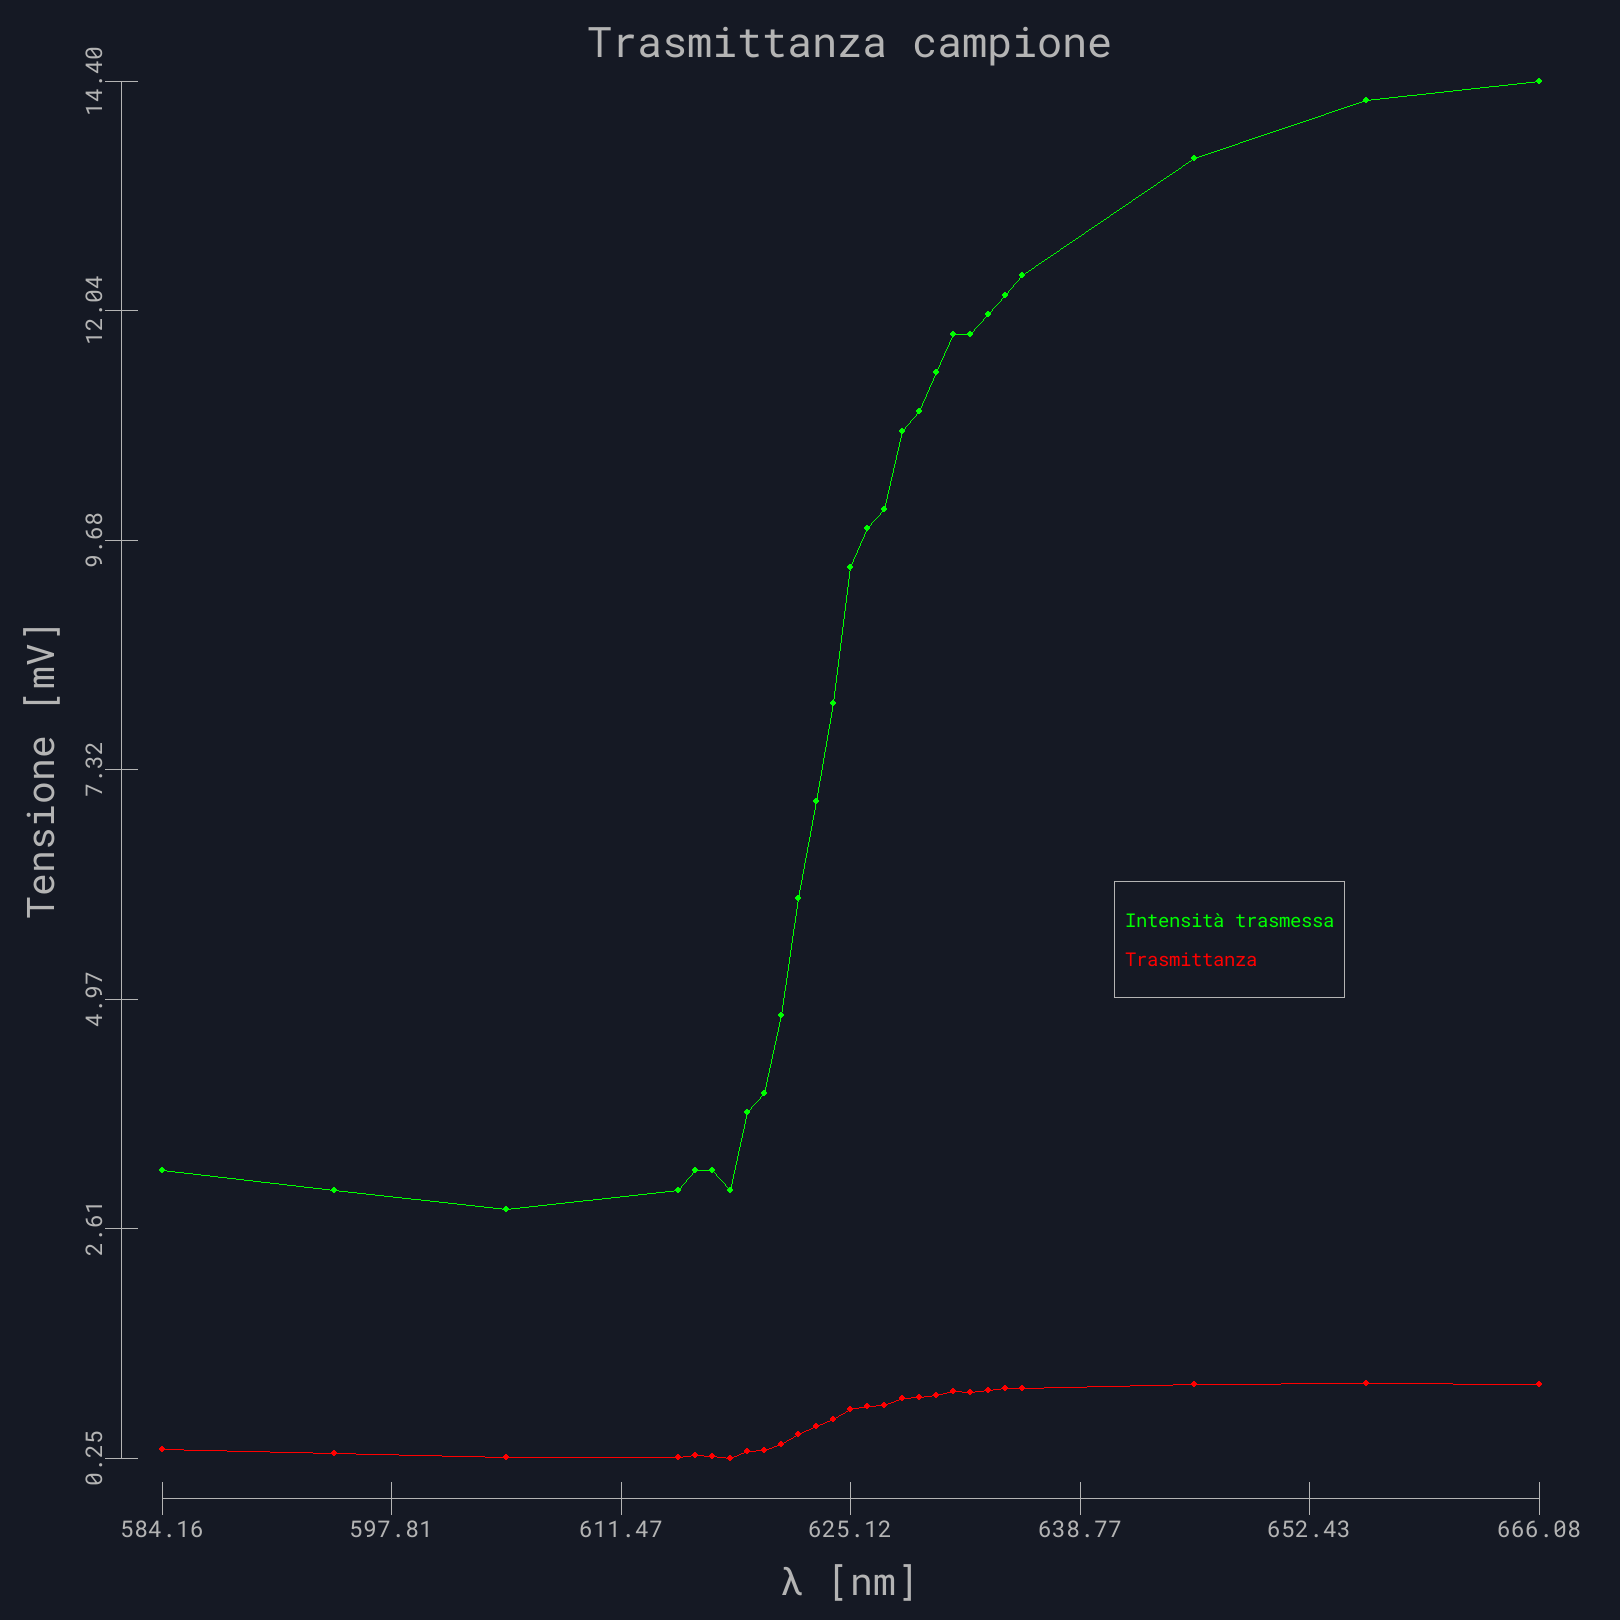
\includegraphics[width=.32\textwidth]{../images/grafico10.png}
    \hfill
    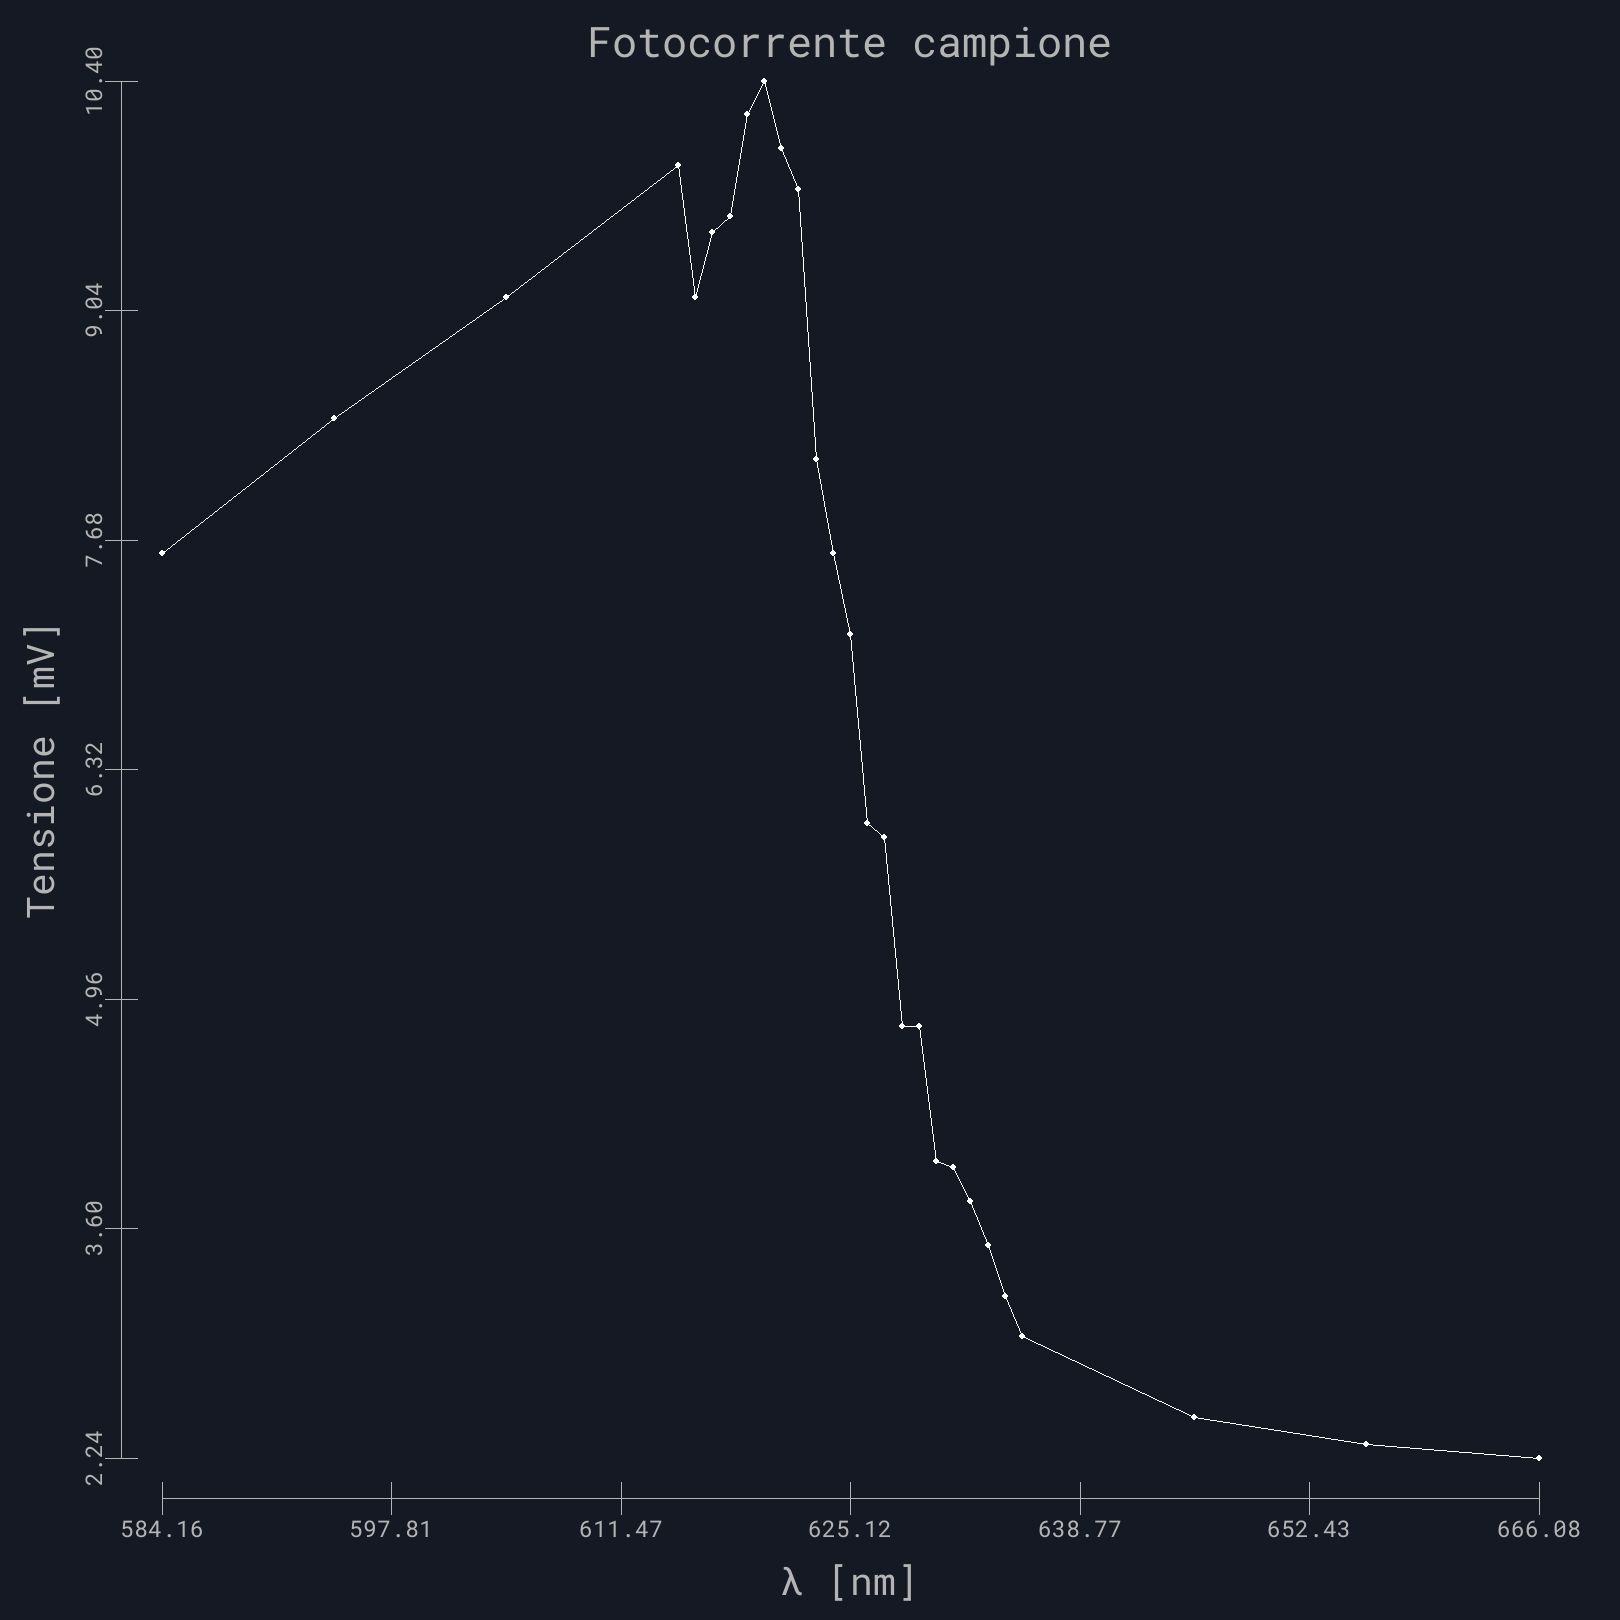
\includegraphics[width=.32\textwidth]{../images/grafico11.png}
    \hfill
    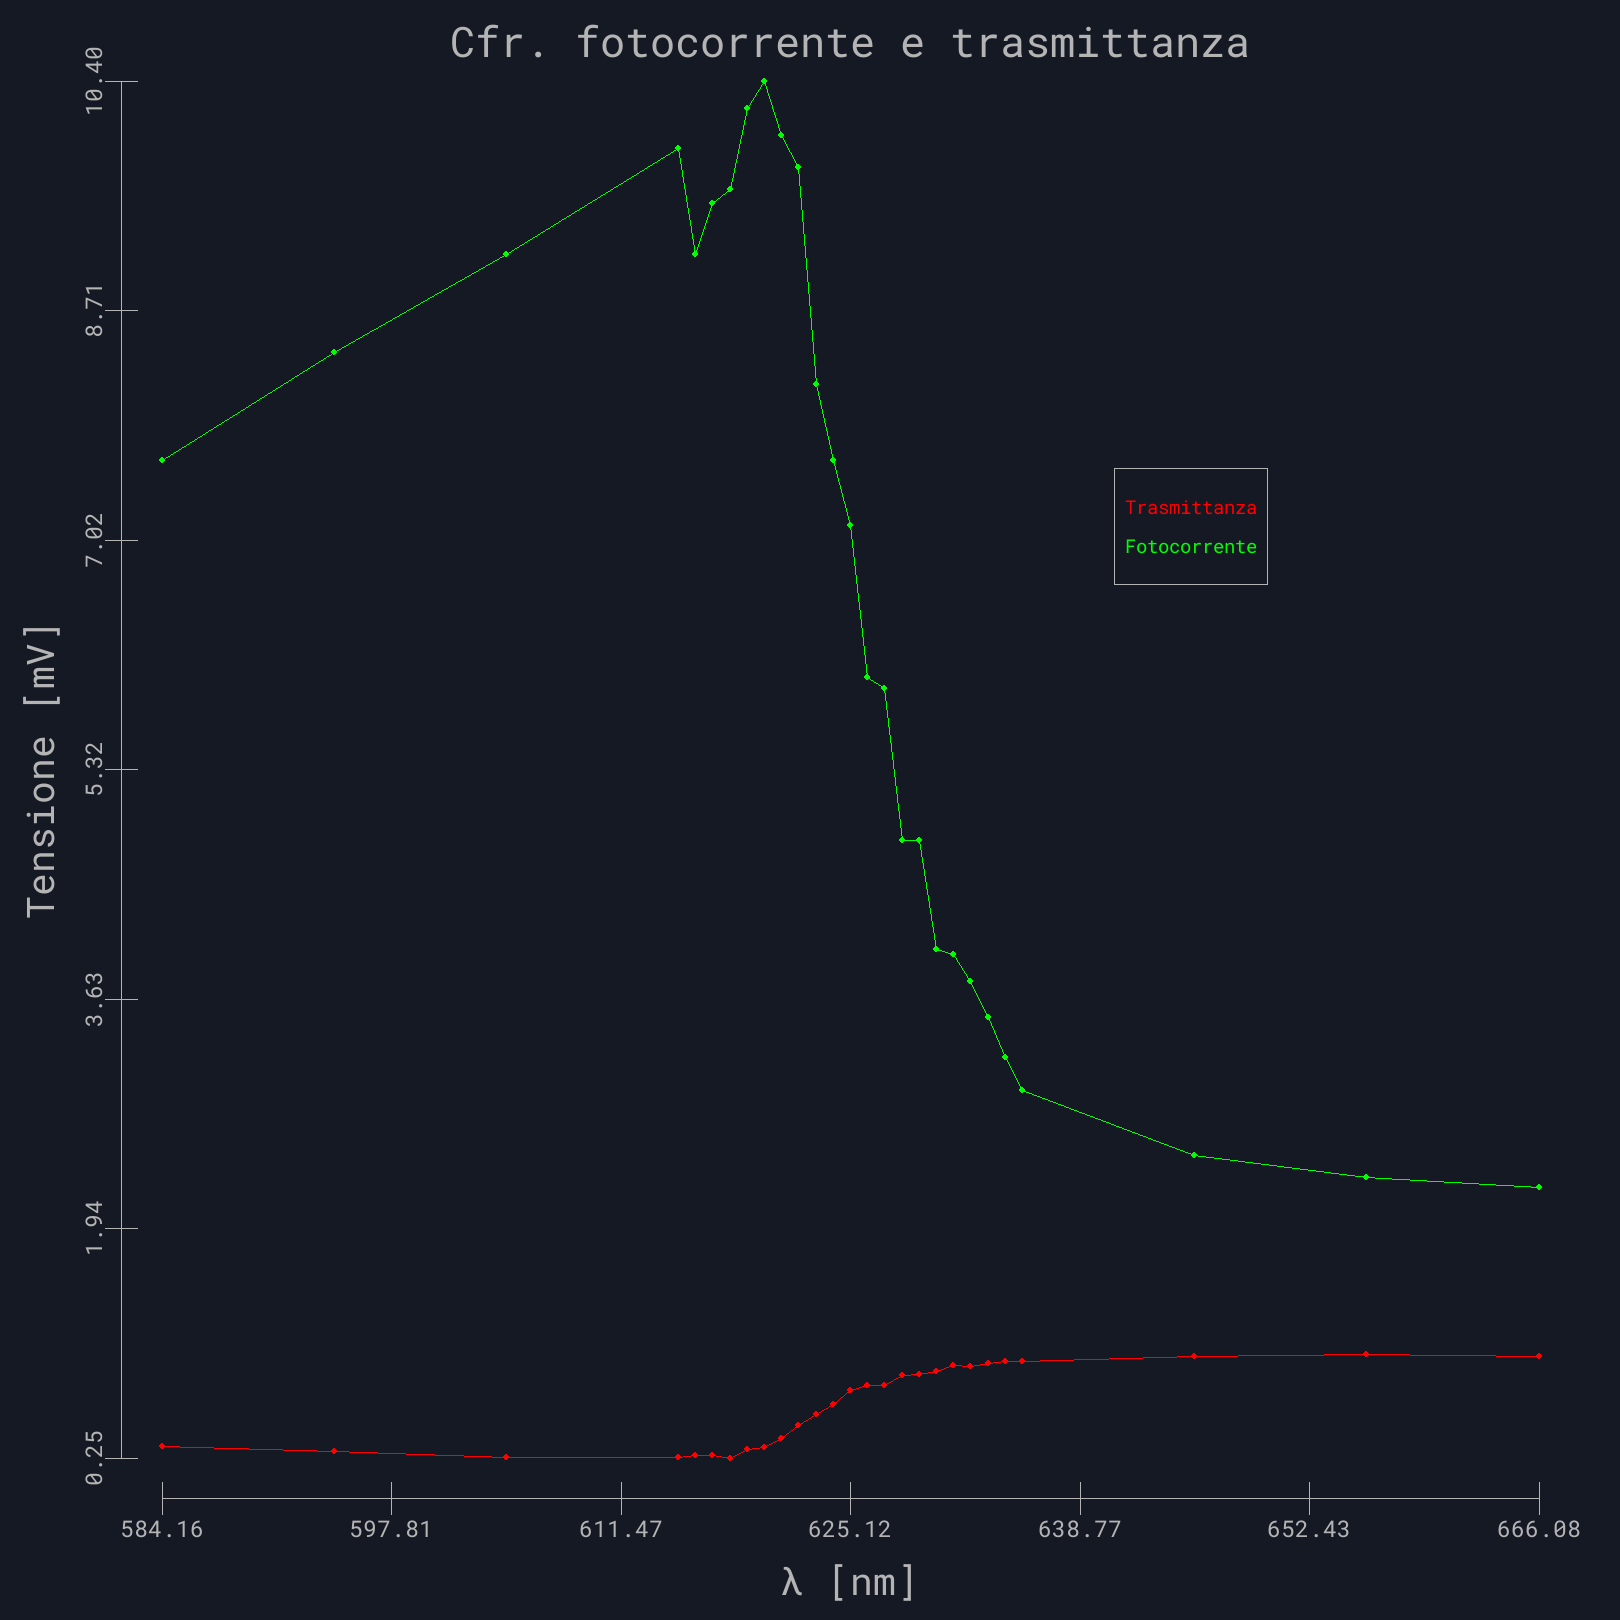
\includegraphics[width=.32\textwidth]{../images/grafico12.png}
    \captionof{figure}{a) Grafico dell'intensità trasmessa $I_t$ e della trasmittanza $\frac{I_t}{I_0}$, b) Grafico della fotocorrente in funzione della lunghezza d'onda, c) Confronto della fotocorrente e della trasmittanza in funzione della lunghezza d'onda.}
    \label{fig:led_grafico}
\end{center}

\subsection{Analisi dati}

\paragraph{Calibrazione dello spettrometro:}
Correlazione pixel-lunghezze d'onda (Figura \ref{grafico:13}): abbiamo calcolato la retta di taratura pixel vs $\lambda$ della lampada. Dati riportati in tabella \ref{tab:tabella7}.
Abbiamo considerato e utilizzato la retta di taratura, invece che i risultati del fit cubico (Figura \ref{grafico:13.2}), a causa del valore del $\chi^2$ (idealmente = 1). Tra le due interpolazioni, il fit lineare restituisce il risultato migliore. Il motivo di un $\chi^2$ così piccolo nel fit cubico risiede nell'ottimo risultato del fit, ma gli errori dei dati così grandi permettono a più cubiche di interpolare i dati, per cui il $\chi^2$ diminusce di valore e dunque lo rende non accettabile. Le calibrazioni future saranno basate sui risultati del fit lineare. 

\paragraph{Calibrazione monocromatore:}
Per trovare a quali lunghezze d'onda corrispondono le unità arbitrarie del monocromatore, abbiamo prima cercato a quali lunghezze d'onda corrispondevano i pixel misurati; per fare questo abbiamo usato la retta di taratura precedente:
$x=(y-b)/a$
dove x è la lunghezza d'onda da estrapolare, y è il valore dei pixel di ogni massimo di ogni picco nello spettro. 

L'errore considerato in questo caso è stato mantenuto come errore percentuale dato che la retta di taratura non copre i valori prossimi a quelli degli errori.

Abbiamo quindi ottenuto un set di lunghezze d'onda a cui corrisponde ogni valore di unità arbitrarie impostato sul monocromatore (si veda tabella \ref{tab:tabella6}).

Con queste corrispondenze abbiamo effettuato un fit per poter estrapolare ogni lunghezza d'onda per qualsiasi valore di unità arbitraria(si veda la figura 15).

\begin{center}
    \begin{minipage}{0.45\textwidth} % Adjust the width as needed
        \centering
        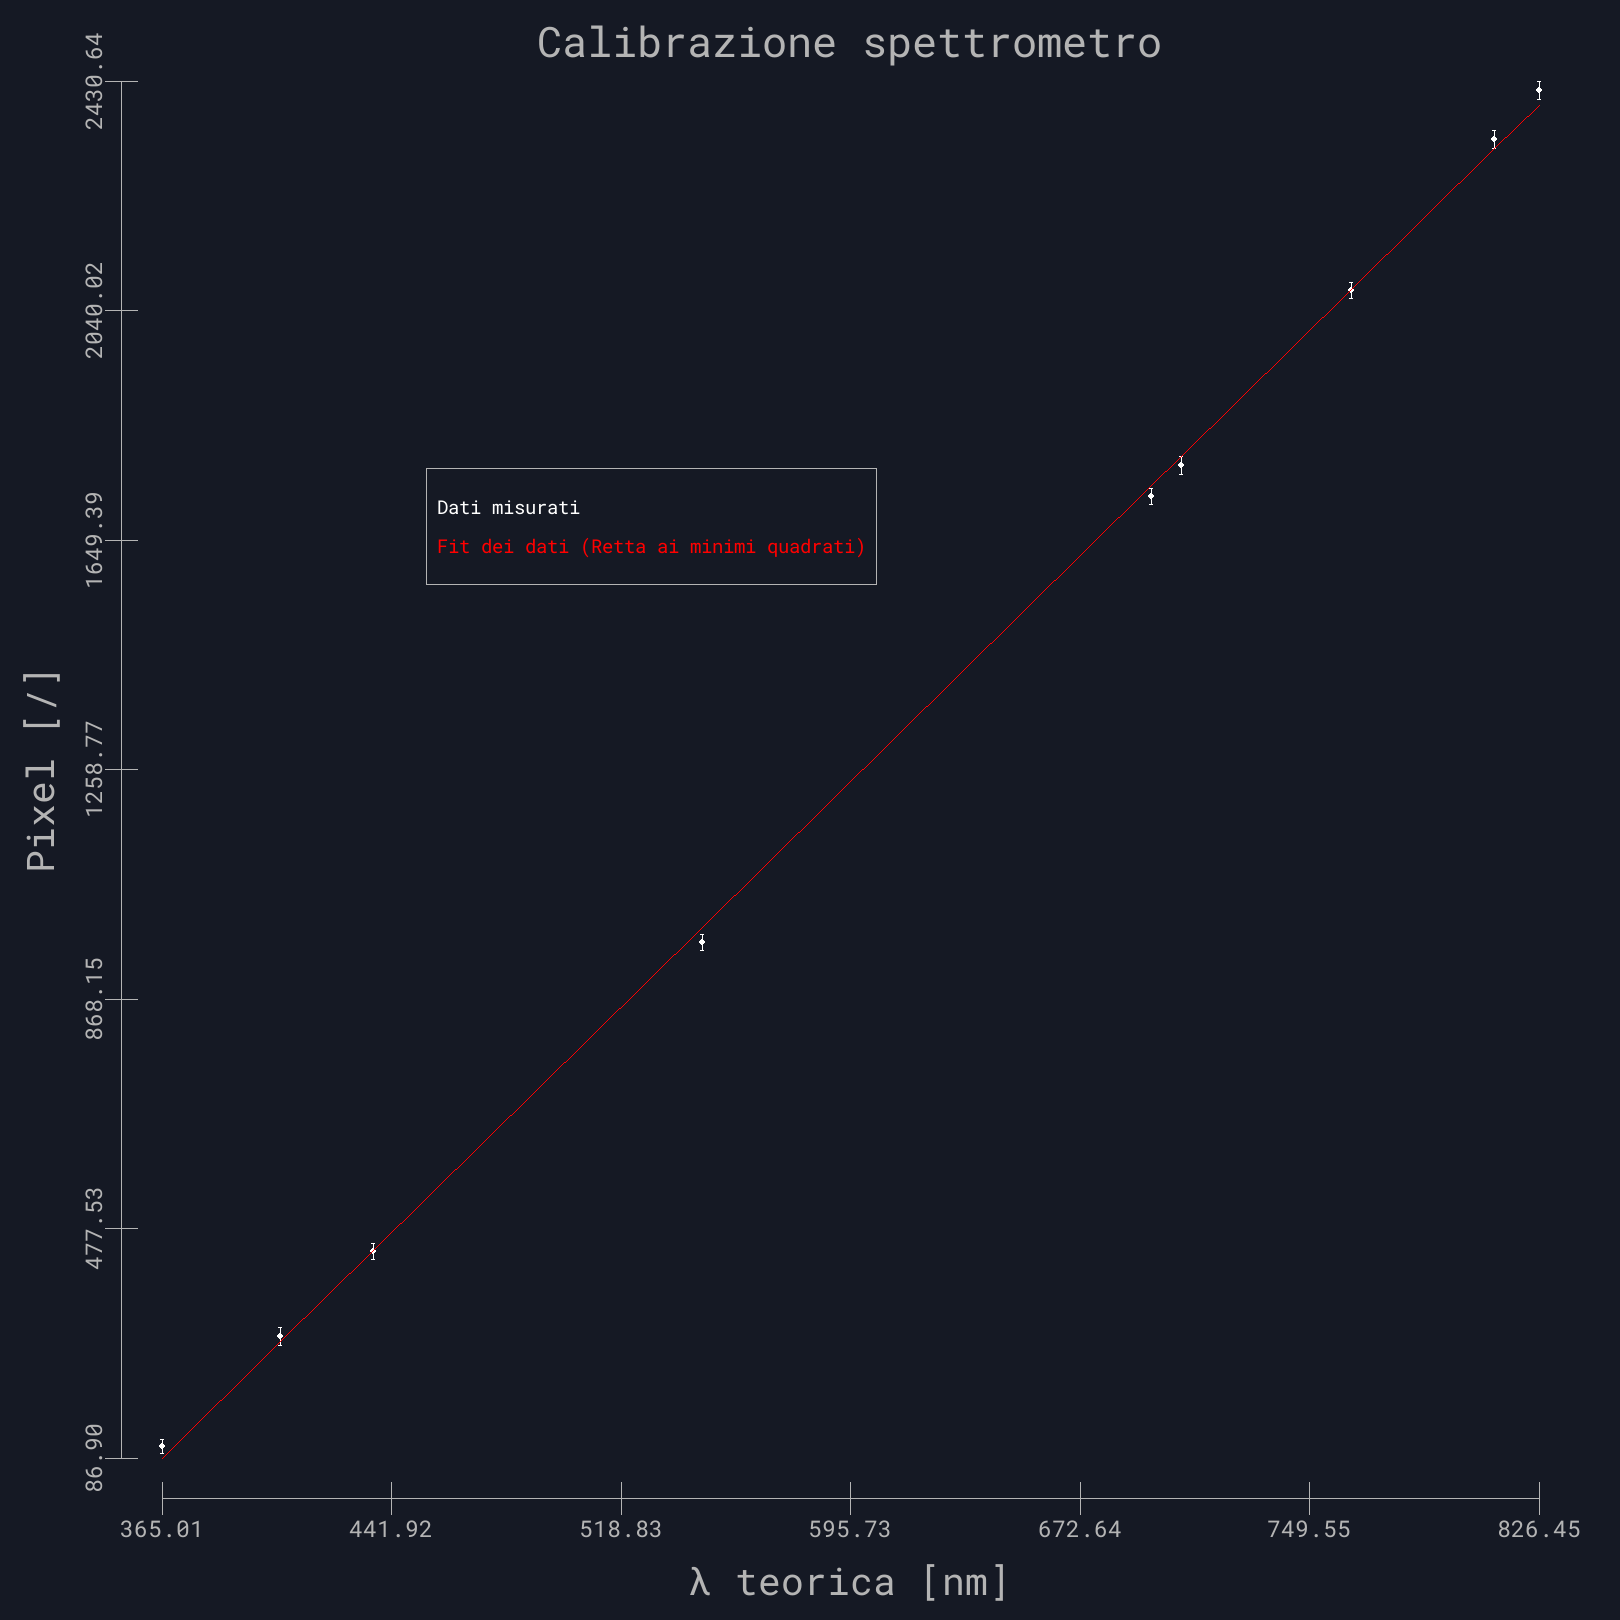
\includegraphics[width=1\linewidth]{../images/grafico13.png} % Replace example-image with your figure filename
        \captionof{figure}{Retta di calibrazione dello spettrometro (software)}
        \label{grafico:13}
    \end{minipage}
    \begin{minipage}{0.45\textwidth} % Adjust the width as needed
        \centering
        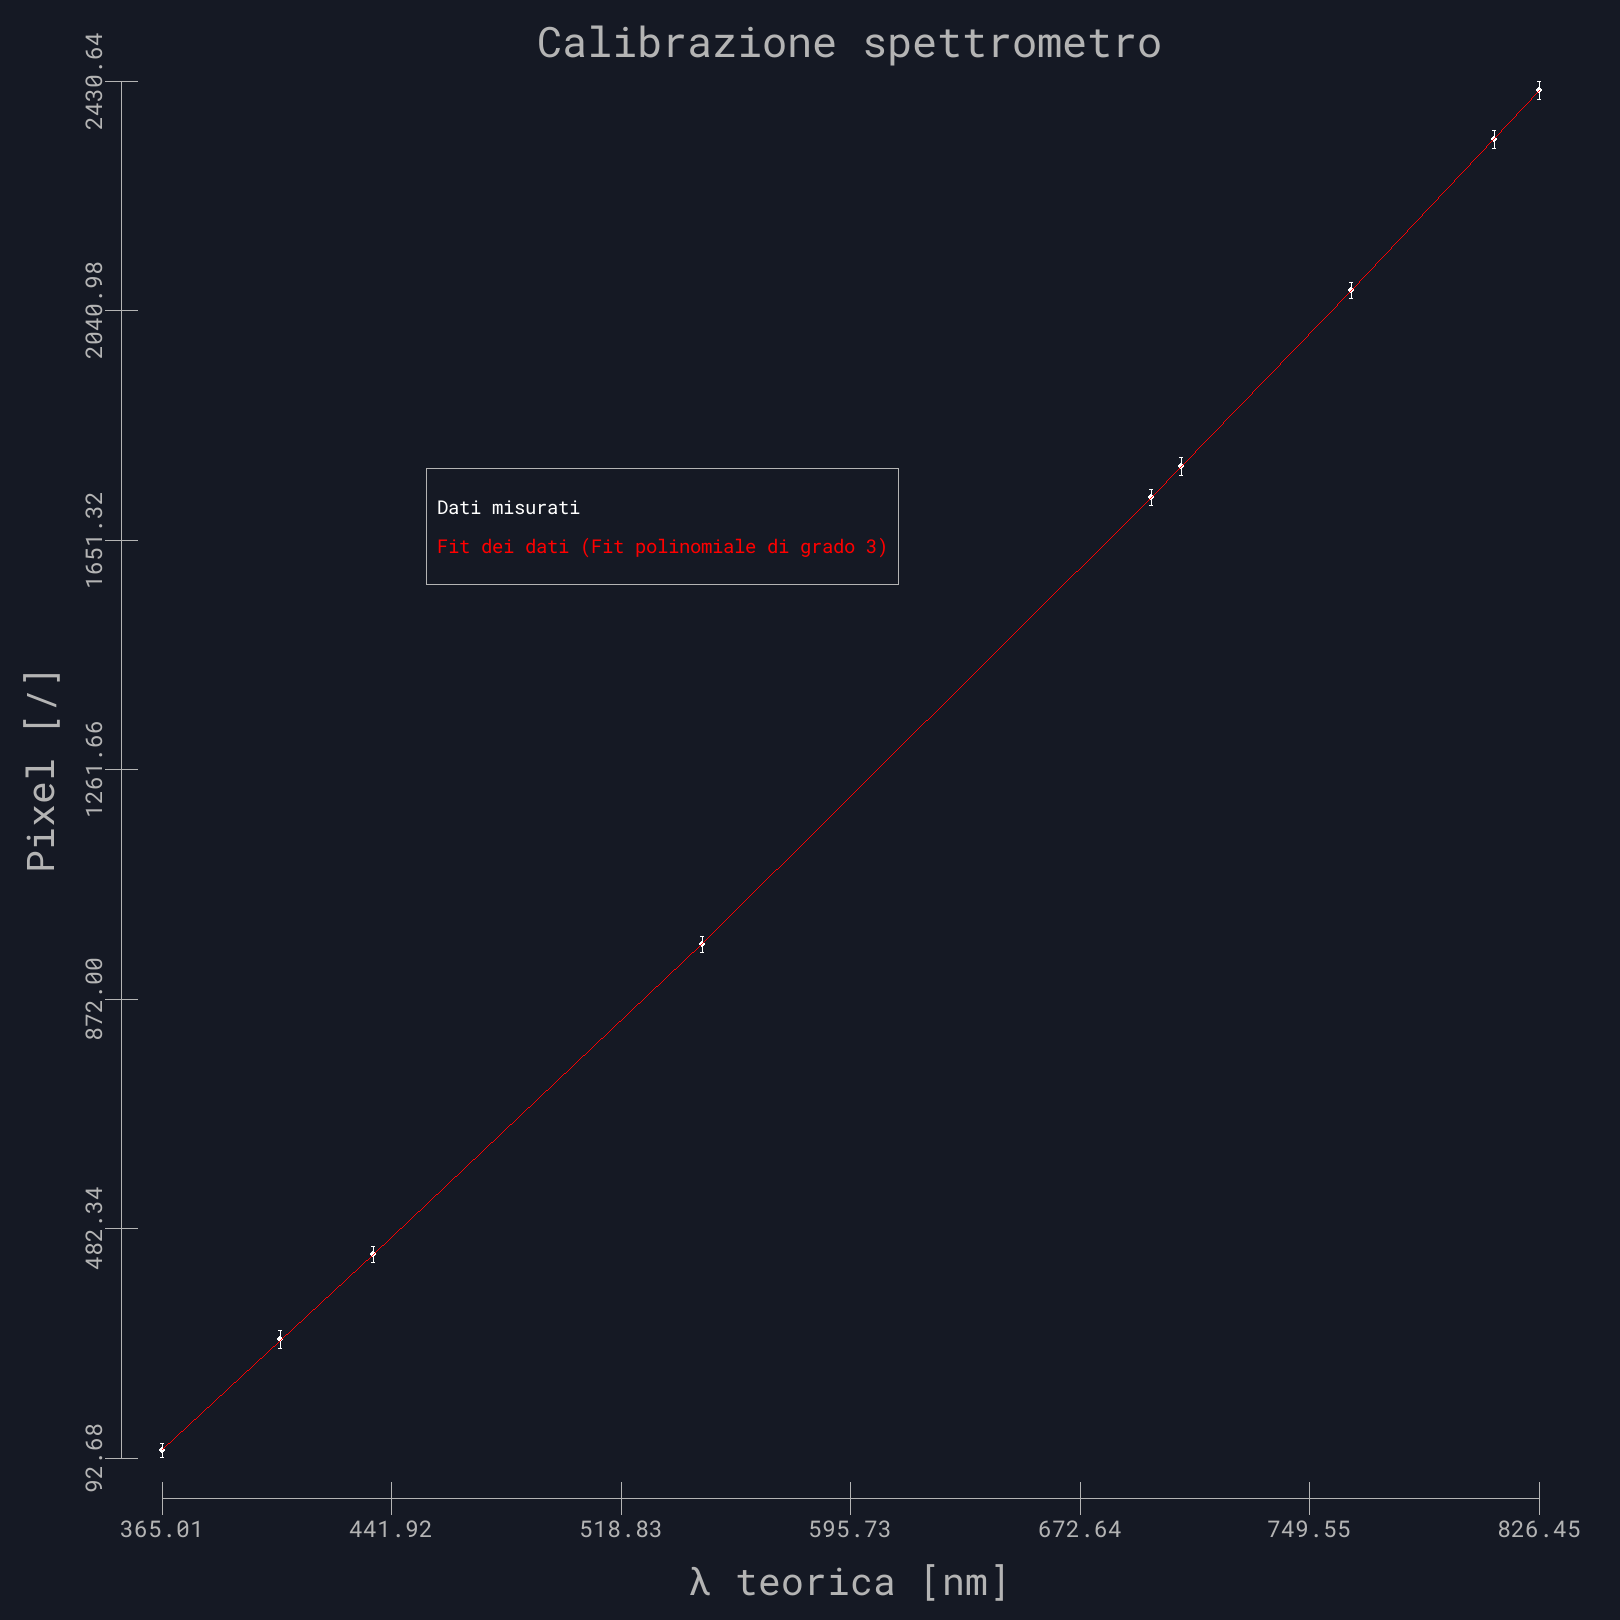
\includegraphics[width=1\linewidth]{../images/grafico13_2.png} % Replace example-image with your figure filename
        \captionof{figure}{Fit cubico di calibrazione dello spettrometro (software) (Parametro b = 0.00029 $\pm$ 0.0005)}
        \label{grafico:13.2}
    \end{minipage}
    \hfill % Add horizontal space between minipages
\end{center}

\begin{center}
    \begin{minipage}{0.4\textwidth}
        \begin{itemize}
            \item $a=(4.99\pm0.04) nm^{-1}$
            \item $b=-1730\pm20$
            \item $\chi^2=1.764$
        \end{itemize}
    \end{minipage}
    \hfill
    \begin{minipage}{0.4\textwidth}
        \begin{itemize}
            \item $c=4.26\pm0.29$
            \item $d=-1501\pm55$
            \item $\chi^2=0.01$
        \end{itemize}
    \end{minipage}
\end{center}


\begin{center}
    \begin{minipage}{0.6\textwidth} % Adjust the width as needed
        \centering
        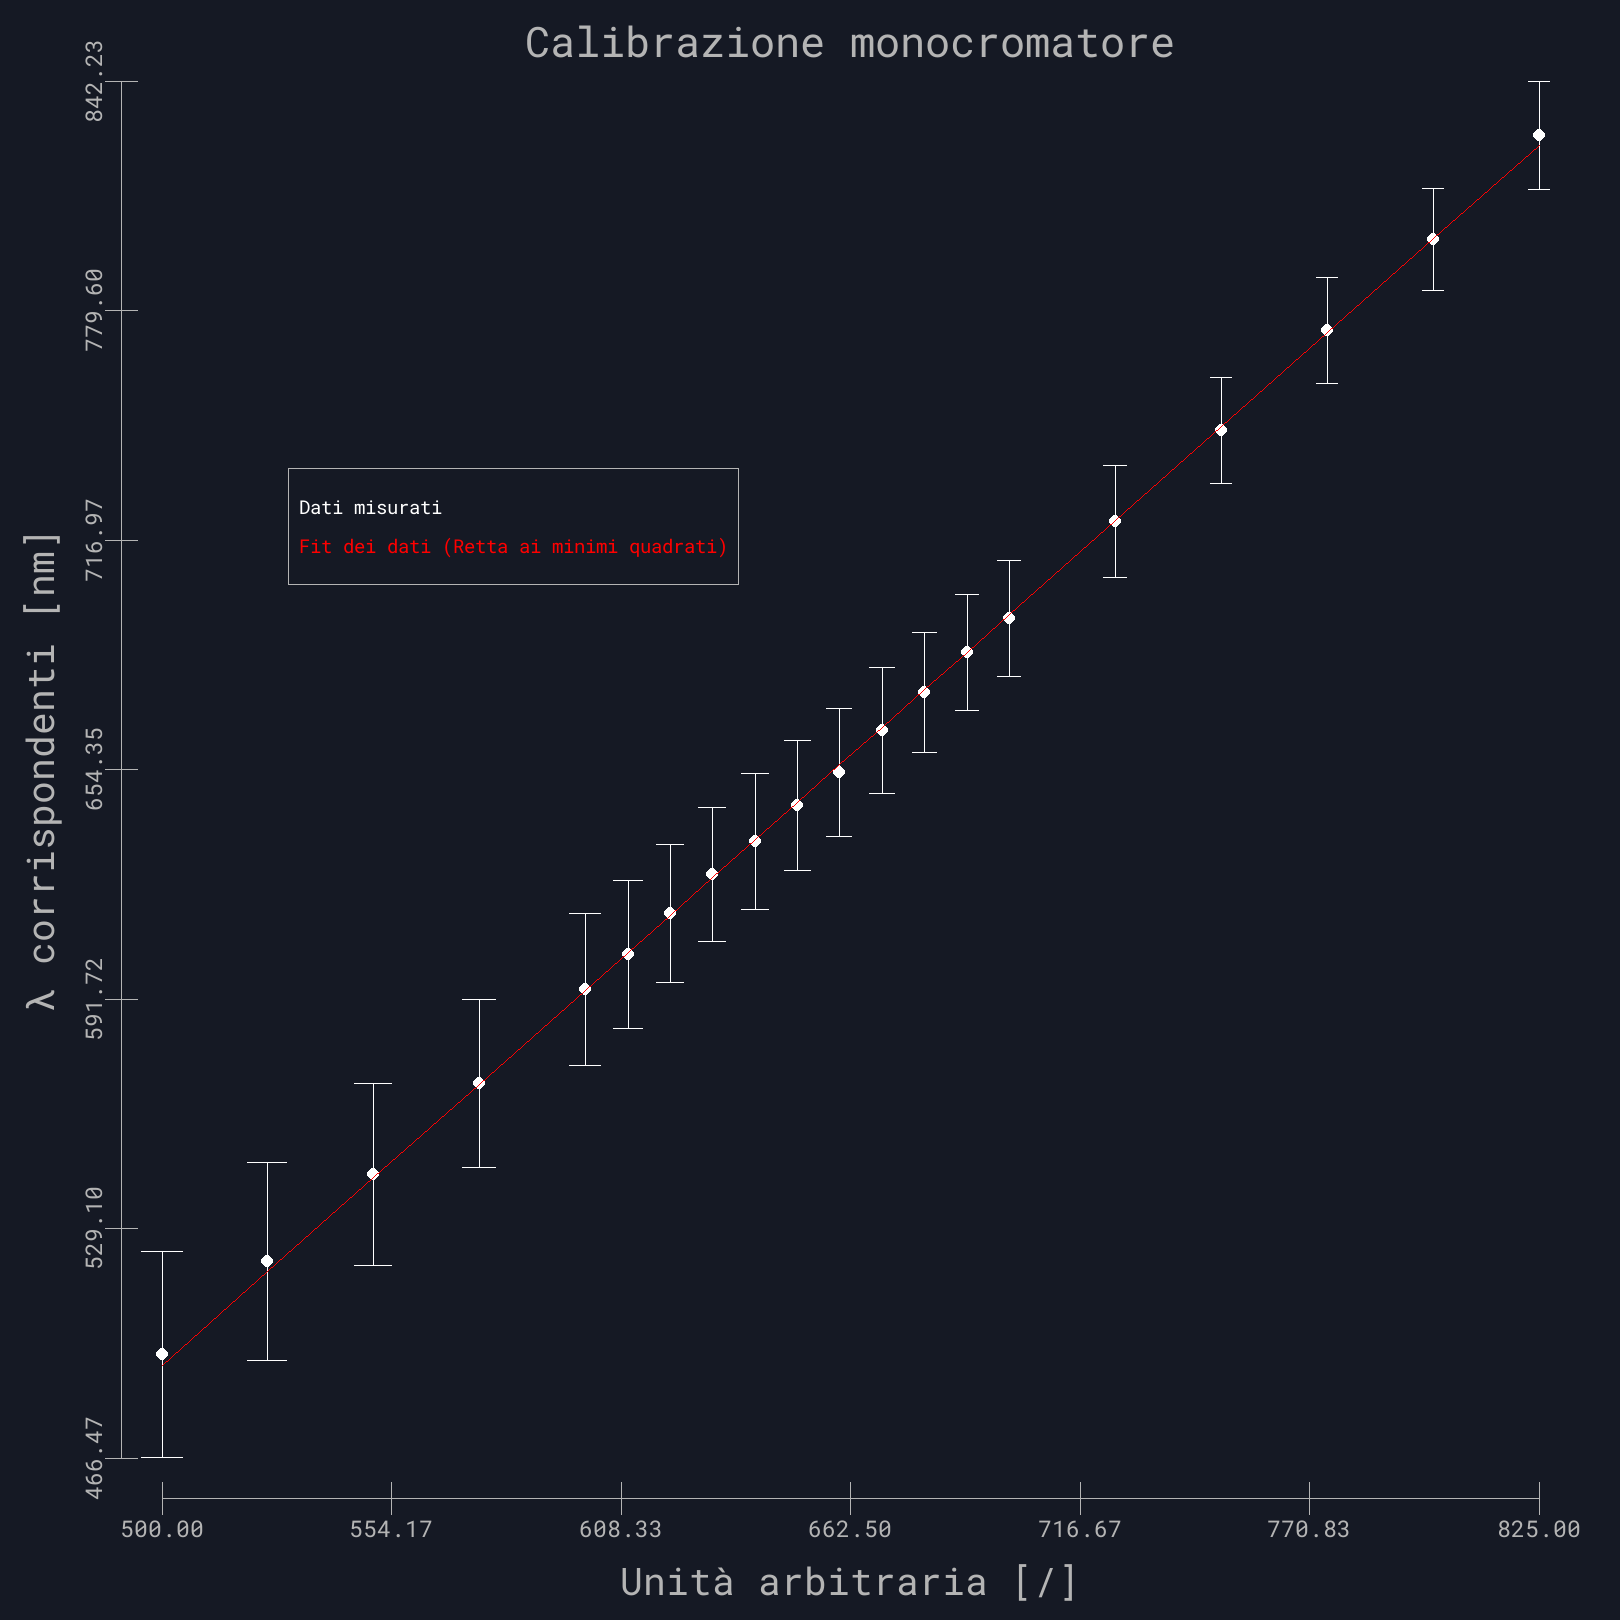
\includegraphics[width=1\linewidth]{../images/grafico14.png} % Replace example-image with your figure filename
        \captionof{figure}{Retta di calibrazione del monocromatore (hardware)}
        \label{grafico:14}
    \end{minipage}
    \hfill % Add horizontal space between minipages
    \begin{minipage}{0.25\textwidth}    
    \begin{itemize}
        \item $a=1.025\pm0.003$
        \item $b=(-21\pm2) nm$
        \item $\chi^2=0.005$
    \end{itemize}
    \end{minipage}
\end{center}
\newpage

\paragraph{Misura dello spettro di riferimento:}
% Effettuando la misura di trasmittanza e fotocorrente del campione, ci siamo accorti che era necessario un infittimento dei dati dello spettro di riferimento tra 620 e 640 unità arbitrarie, ma una volta rimosso il campione dall'apparato per prendere questi nuovi dati, abbiamo avuto difficoltà a riallineare la luce filtrata dal monocromatore al fotodiodo; quindi, abbiamo avvicinato di molto il fotodiodo al monocromatore, ottenendo così valori di corrente molto più alti. Per avere quindi dei valori analoghi a quelli del resto della misura, dato che l'andamento rimane invariato, abbiamo usato una retta di taratura ($R^2=0.953$, $a=(0.44\pm0.10)\frac{1}{mV}$, $b= (0\pm2 mV)$). Lo spettro di riferimento ottenuto è il seguente (dati riportati nelle tabelle \ref{tab:tabella8} e infittimento \ref{tab:tabella9}):
Una volta effettuata la misura dello spettro della lampada, abbiamo dovuto reinfittire il range di lunghezze d'onda dove cadeva il campione. Per farlo abbiamo rimontato il circuito in maniera più compatta per permettere una lettura più accurata dei dati. Dato che la geometria del setup influenza i valori di intensità rilevati, l'andamento dei dati rimane lo stesso ma risultano completamente fuori scala, quindi abbiamo dovuto riassestarli. Per farlo abbiamo usato un fit lineare ($R^2=0.953$, $a=(0.44\pm0.10)\frac{1}{mV}$, $b= (0\pm2 mV)$) di 3 punti che cadevano già in quel range, e che quindi ci hanno dato una linea guida sui valori da seguire, dato che la zona di infittimento era pressochè lineare.

\begin{center}
    \begin{minipage}{0.4\textwidth} % Adjust the width as needed
        \centering
        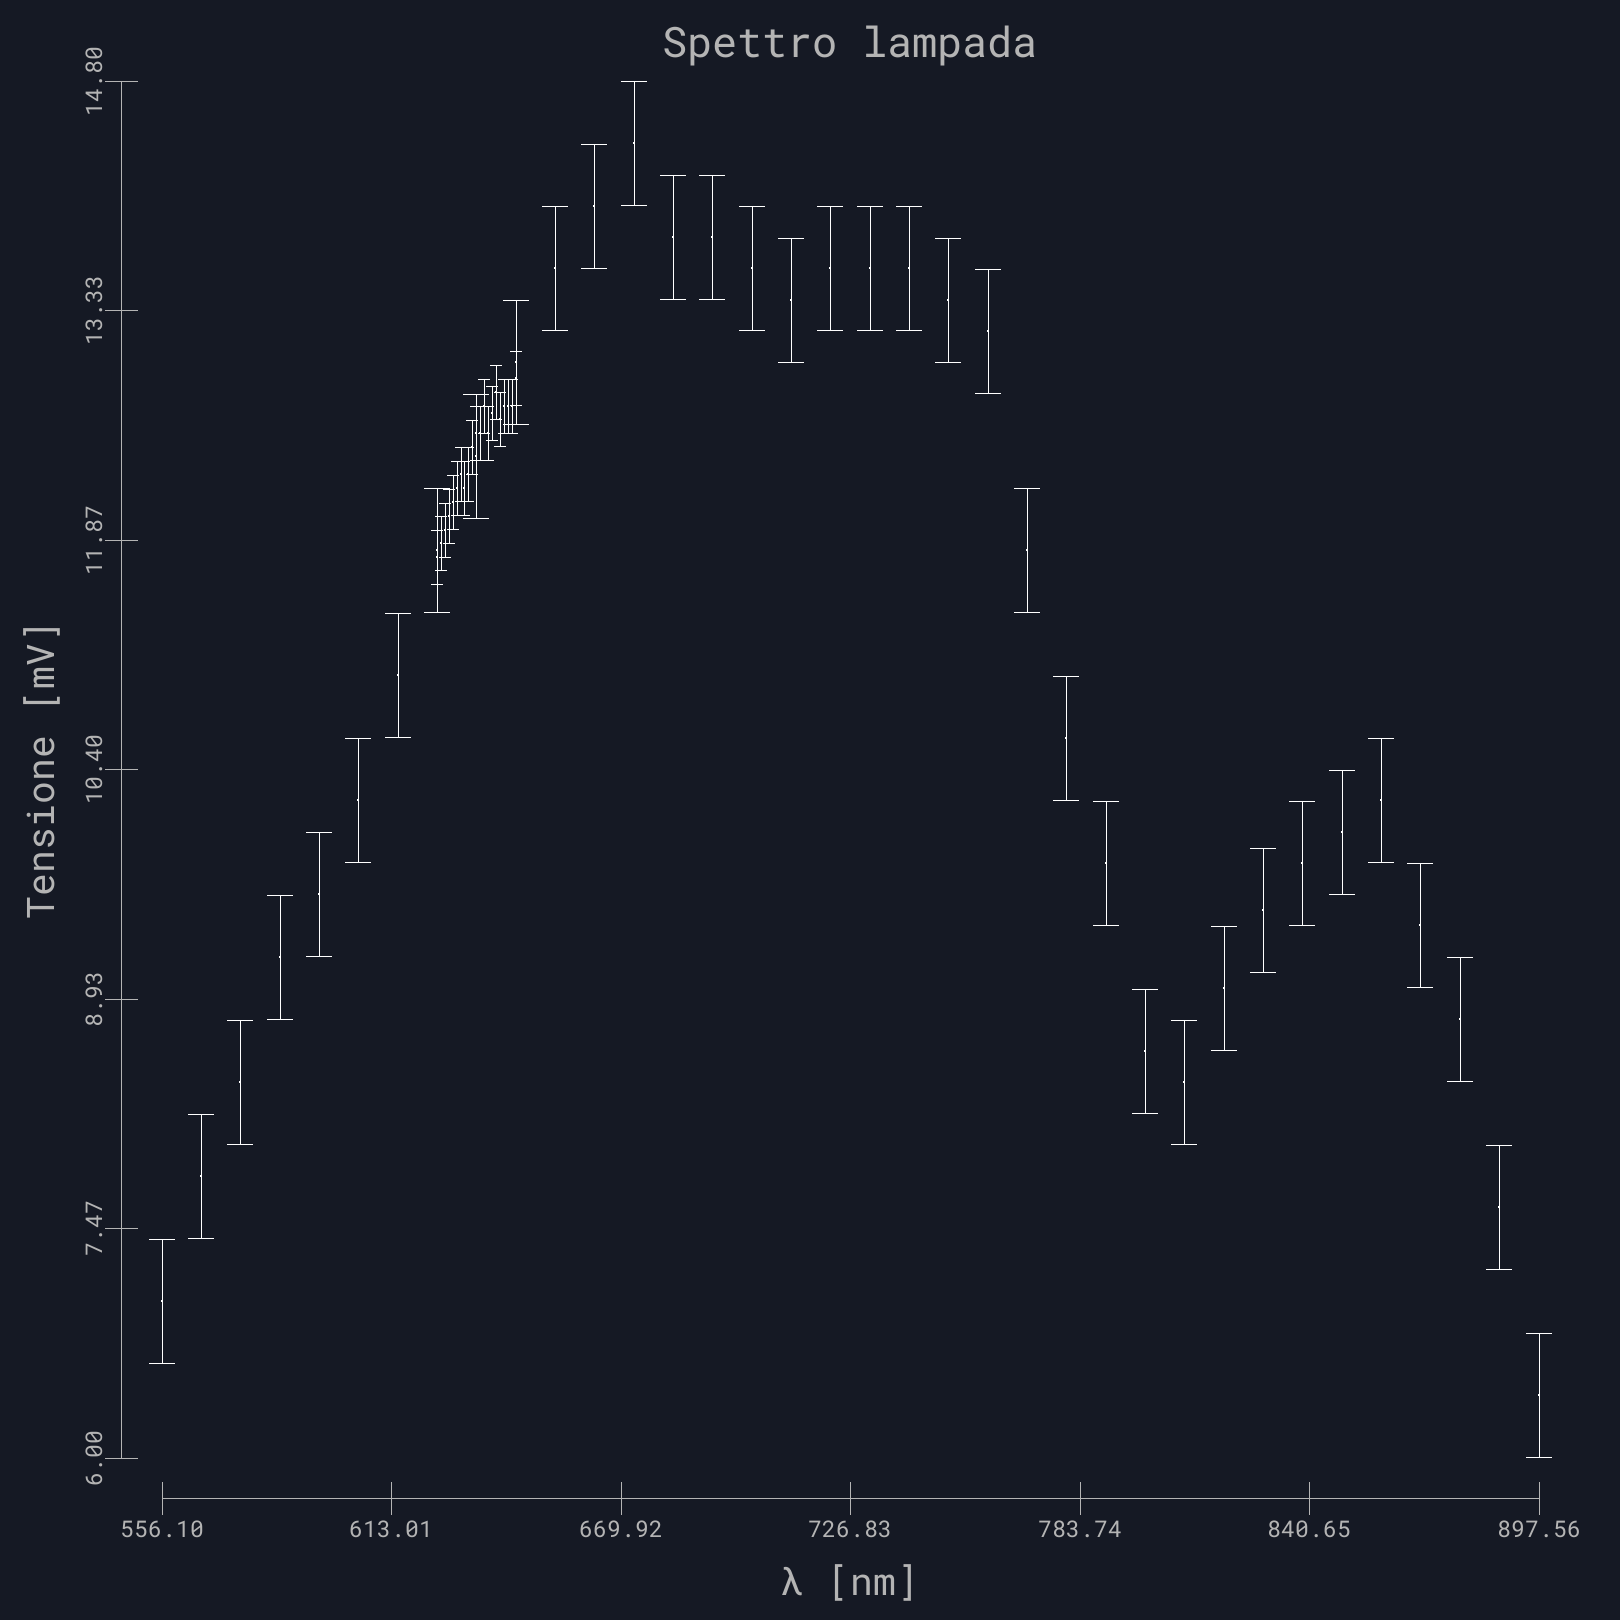
\includegraphics[width=1\linewidth]{../images/grafico15.png} % Replace example-image with your figure filename
        \captionof{figure}{$I_0$ in funzione della lunghezza d'onda.}
        \label{grafico:15}
    \end{minipage}
    \hfill % Add horizontal space between minipages
    \begin{minipage}{0.25\textwidth}    
    \end{minipage}
\end{center}
Con questi dati abbiamo potuto calcolare la trasmittanza e la fotocorrente normalizzata.

\paragraph{Misura di trasmittanza e fotocorrente:} Grafico andamento della trasmittanza e fotocorrente normalizzate per permettere un confronto visivo:

\begin{center}
    \begin{minipage}{0.4\textwidth} % Adjust the width as needed
        \centering
        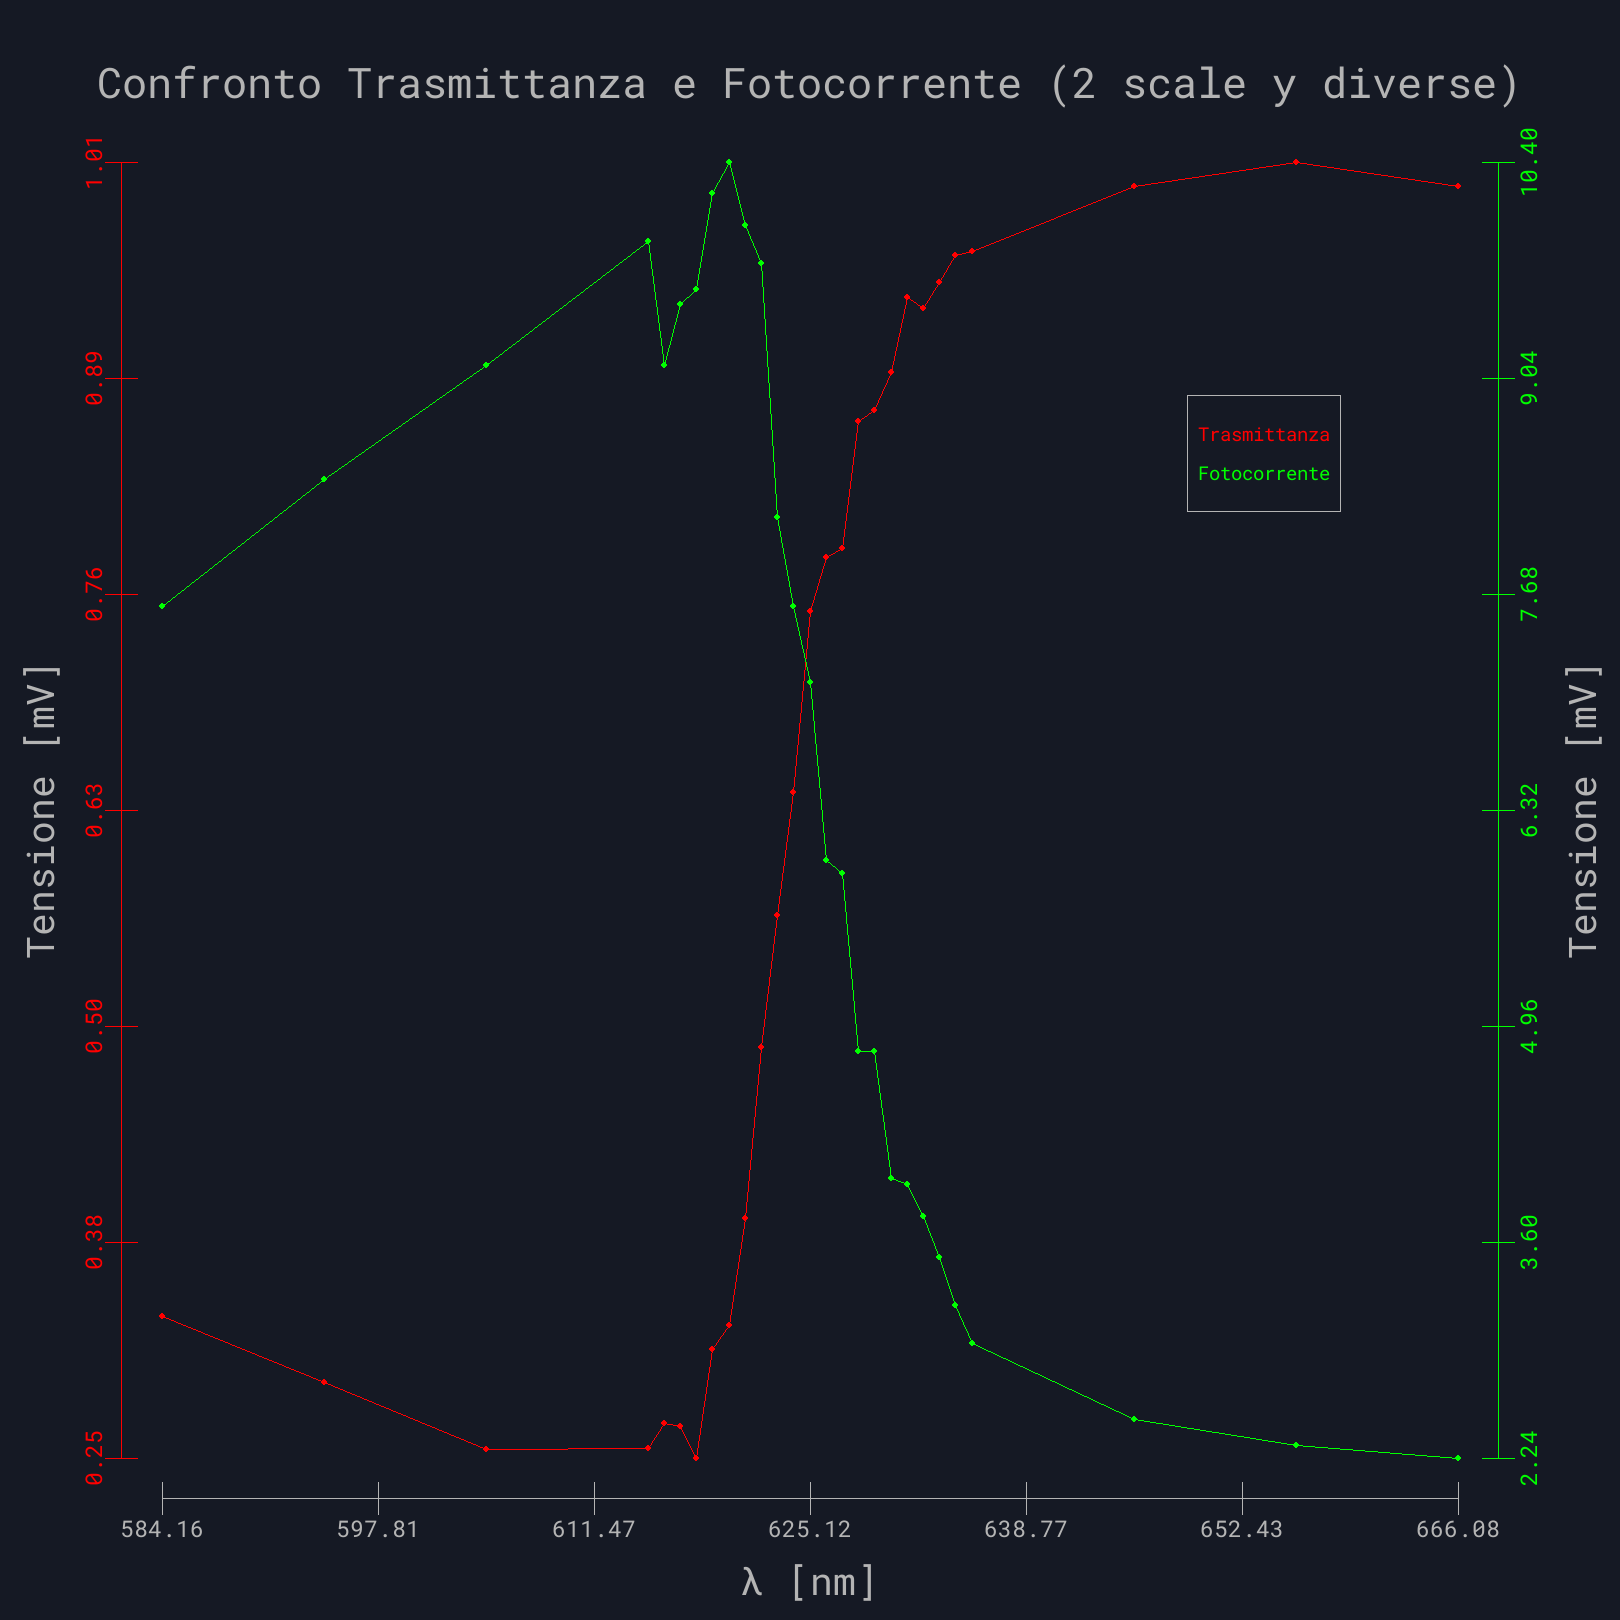
\includegraphics[width=1\linewidth]{../images/grafico16.png} % Replace example-image with your figure filename
        \captionof{figure}{Grafico di fotocorrente e trasmittanza, normalizzate e sovrapposte}
        \label{grafico:16}
    \end{minipage}    
\end{center}

\subsubsection{Calcolo del flesso della fotocorrente e della trasmittanza:}

\begin{center}
    \begin{minipage}{0.4\textwidth}
        \paragraph{Primo metodo:} massimo della derivata. Il fit della derivata corrisponde ad una gaussiana.
        $y= dV/d\lambda \quad \quad x=\lambda$
    \end{minipage}
    \hfill
    \begin{minipage}{0.4\textwidth}
        \paragraph{Secondo metodo:} fit della curva con una sigmoide.
        \newline
        $S(\lambda) = b + \frac{A}{1+\exp(\pm\frac{\lambda- \lambda_0}{\Delta\lambda})}$
    \end{minipage}
\end{center}
\begin{center}
    \begin{minipage}{0.4\textwidth}
        \paragraph{Ch 1 non normalizzato:}
        \begin{itemize}
            \item Mean: 625.1645056248408 
            \item Standard Deviation: 10.970706530478989
            \item Lunghezza d'onda:  $(625,2 \pm11,0)nm$ 
            \item $E_g=(  1,98\pm0,03  )eV$
        \end{itemize}
    \end{minipage}
    \hfill
    \begin{minipage}{0.4\textwidth}
        \paragraph{Ch 1 non normalizzato:}
        \begin{itemize}
            \item $\lambda_0: 624.528019861369$
            \item $\Delta_\lambda: 3.151767216307566$
            \item Lunghezza d'onda:  $(625 \pm3)nm$
            \item $E_g=(  1,984\pm0,010  )eV$
        \end{itemize}
    \end{minipage}
\end{center}
\hrulefill
\begin{center}
    \begin{minipage}{0.4\textwidth}
        \paragraph{Ch 1 normalizzato:}
        \begin{itemize}
            \item Mean: 625.2883483286292
            \item Standard Deviation: 12.37392154208691
            \item Lunghezza d'onda:  $(625 \pm12)nm$
            \item $E_g=(  1,98\pm 0,04 )eV$
        \end{itemize}
    \end{minipage}
    \hfill
    \begin{minipage}{0.4\textwidth}
        \paragraph{Ch 1 normalizzato:}
        \begin{itemize}
            \item $\lambda_0: 623.9500368592087$
            \item $\Delta_\lambda: 2.245275722023942$
            \item Lunghezza d'onda:  $(624 \pm2)nm$
            \item $E_g=(  1,987\pm 0,006 )eV$
        \end{itemize}
    \end{minipage}
\end{center}
\hrulefill
\begin{center}
    \begin{minipage}{0.4\textwidth}
        \paragraph{Ch 2 non normalizzato:}
        \begin{itemize}
            \item Mean: 628.2806686585551
            \item Standard Deviation: 10.837864792387364
            \item Lunghezza d'onda:  $(625,3 \pm10,8)nm$
            \item $E_g=(1,98\pm0,03  )eV$
        \end{itemize}
    \end{minipage}
    \hfill
    \begin{minipage}{0.4\textwidth}
        \paragraph{Ch 2 non normalizzato:}
        \begin{itemize}
            \item $\lambda_0: 626.8199096670963$
            \item $\Delta_\lambda: 2.1117241944834335$
            \item Lunghezza d'onda:  $(627 \pm2)nm$
            \item $E_g=(  1,978\pm 0,006 )eV$
        \end{itemize}
    \end{minipage}
\end{center}
\hrulefill
\begin{center}
    \begin{minipage}{0.4\textwidth}
        \paragraph{Ch 2 normalizzato:}
        \begin{itemize}
            \item Mean: 626.2479509379564
            \item Standard Deviation: 12.696673651440905
            \item Lunghezza d'onda:  $(626 \pm13)nm$
            \item $E_g=(1,98\pm 0,04 )eV$
        \end{itemize}        
    \end{minipage}
    \hfill
    \begin{minipage}{0.4\textwidth}
        \paragraph{Ch 2 normalizzato:}
        \begin{itemize}
            \item $\lambda_0: 626.2788529248645$
            \item $\Delta_\lambda: 2.5898284977240458$
            \item Lunghezza d'onda:  $(626 \pm3)nm$
            \item $E_g=(1,981\pm0,009  )eV$
        \end{itemize}
    \end{minipage}
\end{center}
\hrulefill
\\
Le energy gap sono correlate con un t-test al 95\% di confidenza. Weighted Average Function: $2.0 eV \pm 0.8 eV$.
\\
La differenza tra la $\sigma_{std}$ e la $\Delta\lambda$ risiede innanzitutto sul grafico applicato: il fit gaussiano è stato applicato sulla derivata della funzione, mentre il fit sigmoide direttamente sui dati ottenuti.

\subsection{Propagazione degli errori ($\sigma$): }
Partendo dalla regola generale per la propagazione degli errori con il metodo delle derivate parziali $\sigma_y=\sqrt{\sigma( \frac{\partial y}{\partial x_i}*\sigma_{x_i} )^2 }$
$$\sigma_E=E\frac{\sigma_{\lambda}}{\lambda}$$
Il calcolo degli errori nella retta di taratura del monocromatore per le $\lambda$ è stato fatto in questo modo:\\
Valendo la retta di taratura dello spettrometro solo per $\lambda$ comprese tra $\sim 365nm$ e $\sim 826nm$ non abbiamo potuto trasformare le incertezze delle misure da pixel a nm partendo dalle FWHM.\\
Abbiamo quindi calcolato in percentuale quanto fosse la FWHM rispetto alla propria misura e abbiamo riapplicato lo stesso errore alle nuove misure convertite in nm.

\subsection{Conclusioni}
Dall'andamento della fotocorrente e della trasmittanza possiamo confermare che ad alte energie e quindi basse lunghezze d'onda ci sono bassi valori di trasmittanza e alti valori di fotocorrente perché le energie sono più alte dell'energy gap.  Per basse energie (cioè per quelle minori dell'energy gap del campione, presumibilmente Si   o GaAs) allora abbiamo bassa fotocorrente e alta trasmittanza. I risultati sono buoni e questo viene confermato dal fatto che gli otto valori di lunghezze d'onda da noi calcolati portano circa ad uno stesso punto di flesso ( che corrisponde alla lunghezza d'onda che ci interessa, la quale rispecchia l'energy gap del campione). La bontà della misura è data dal fatto che questi otto valori soddisfano il test di compatibilità.
\\
Uso del chopper: la modulazione del fascio luminoso è servita in modo da poter da effettuare la misura usando l'oscilloscopio che va a corrente alternata.

\newpage
\paragraph{Plot dei fit: }

\begin{center}
    \begin{minipage}{0.25\textwidth}        
        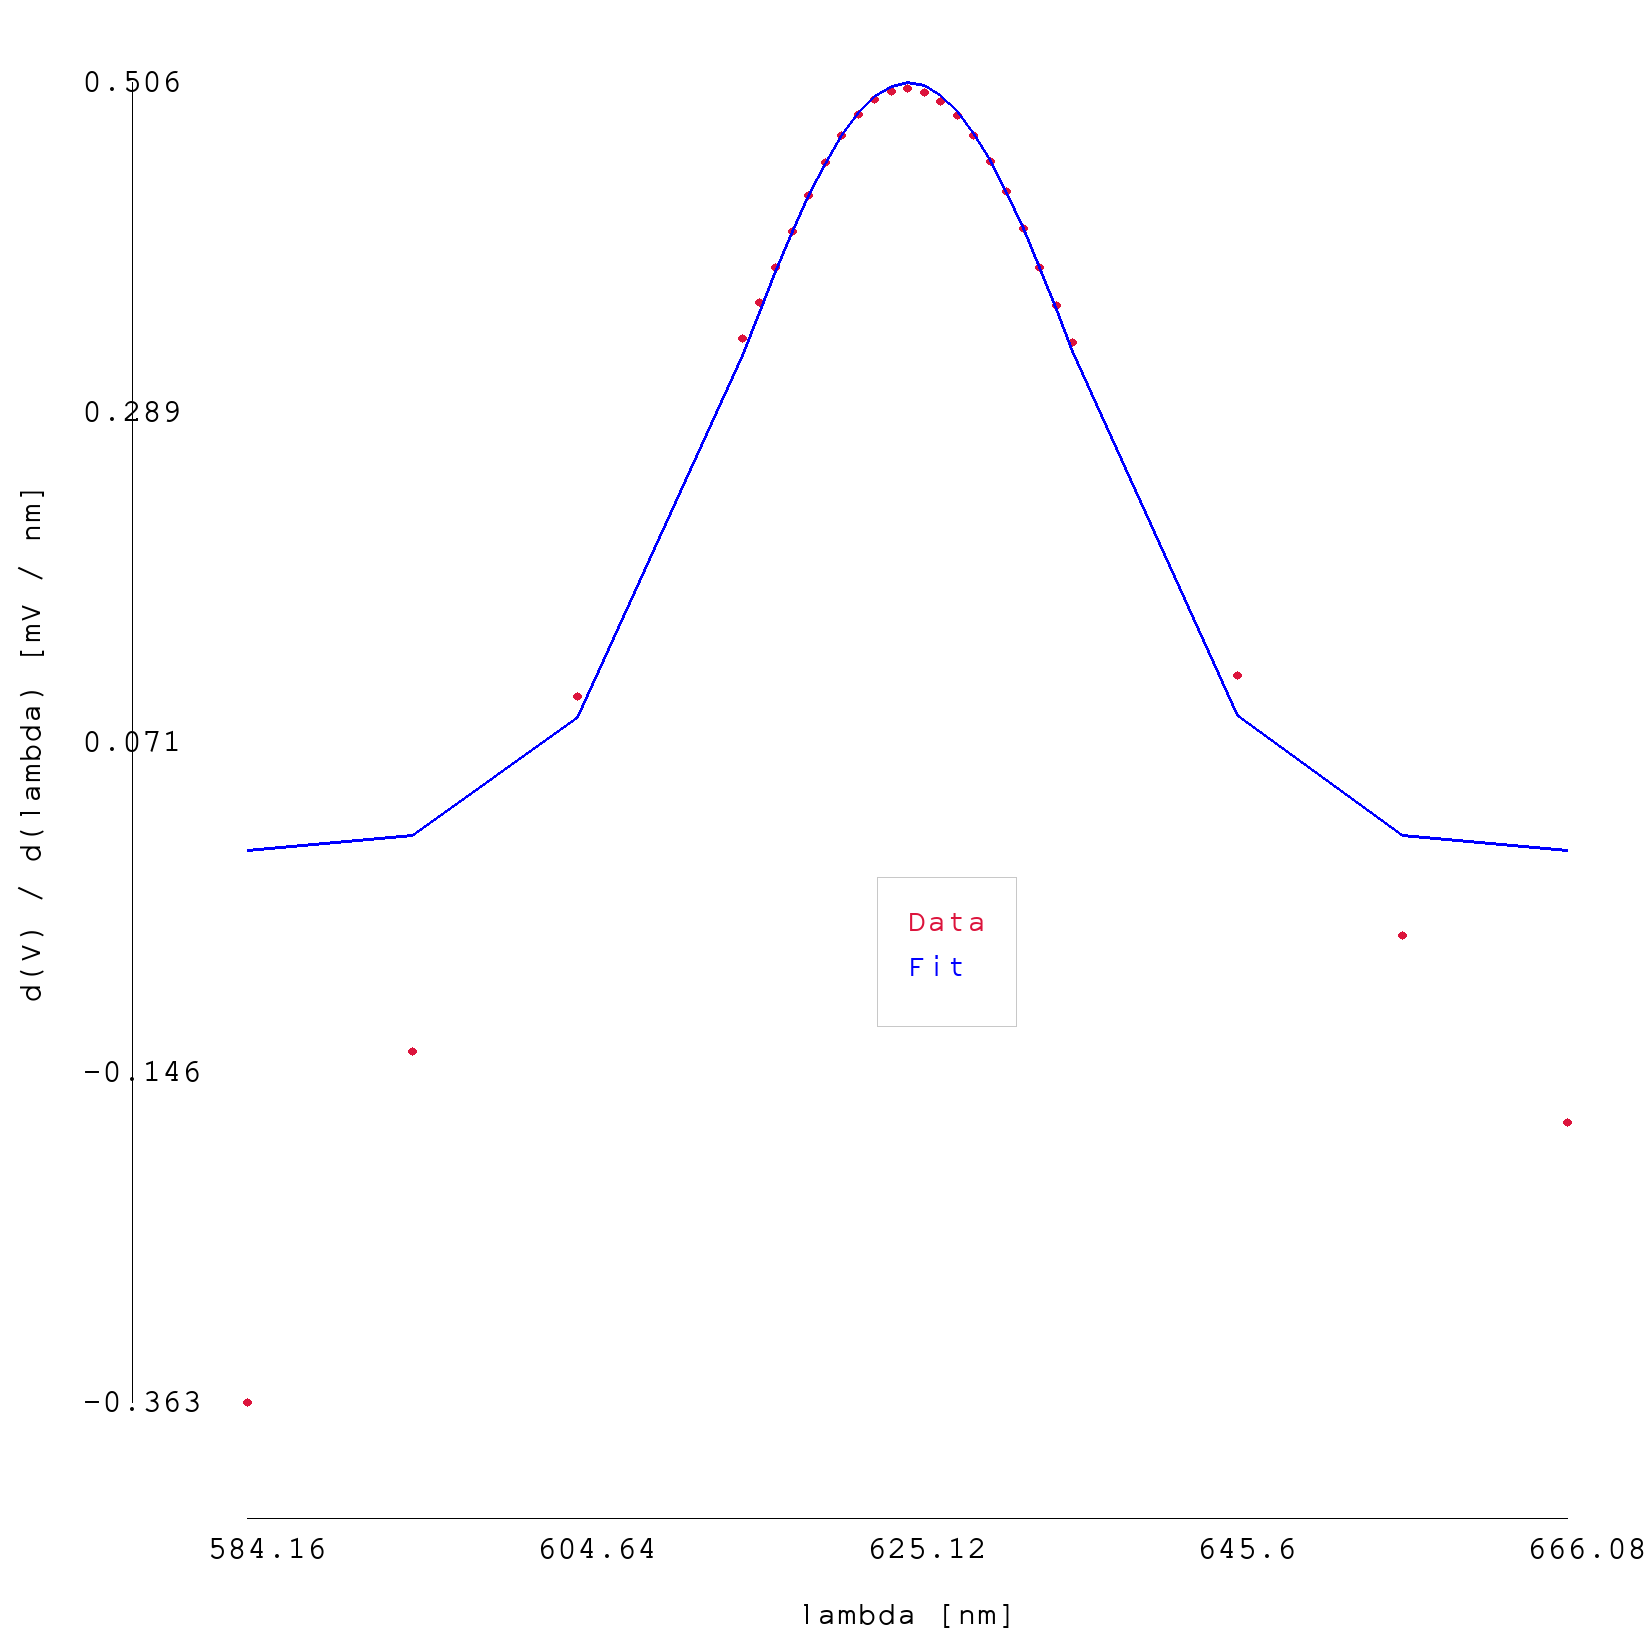
\includegraphics[width=1\linewidth]{../images/grafico1_1.png}
    \end{minipage}
    \hfill
    \begin{minipage}{0.25\textwidth}        
        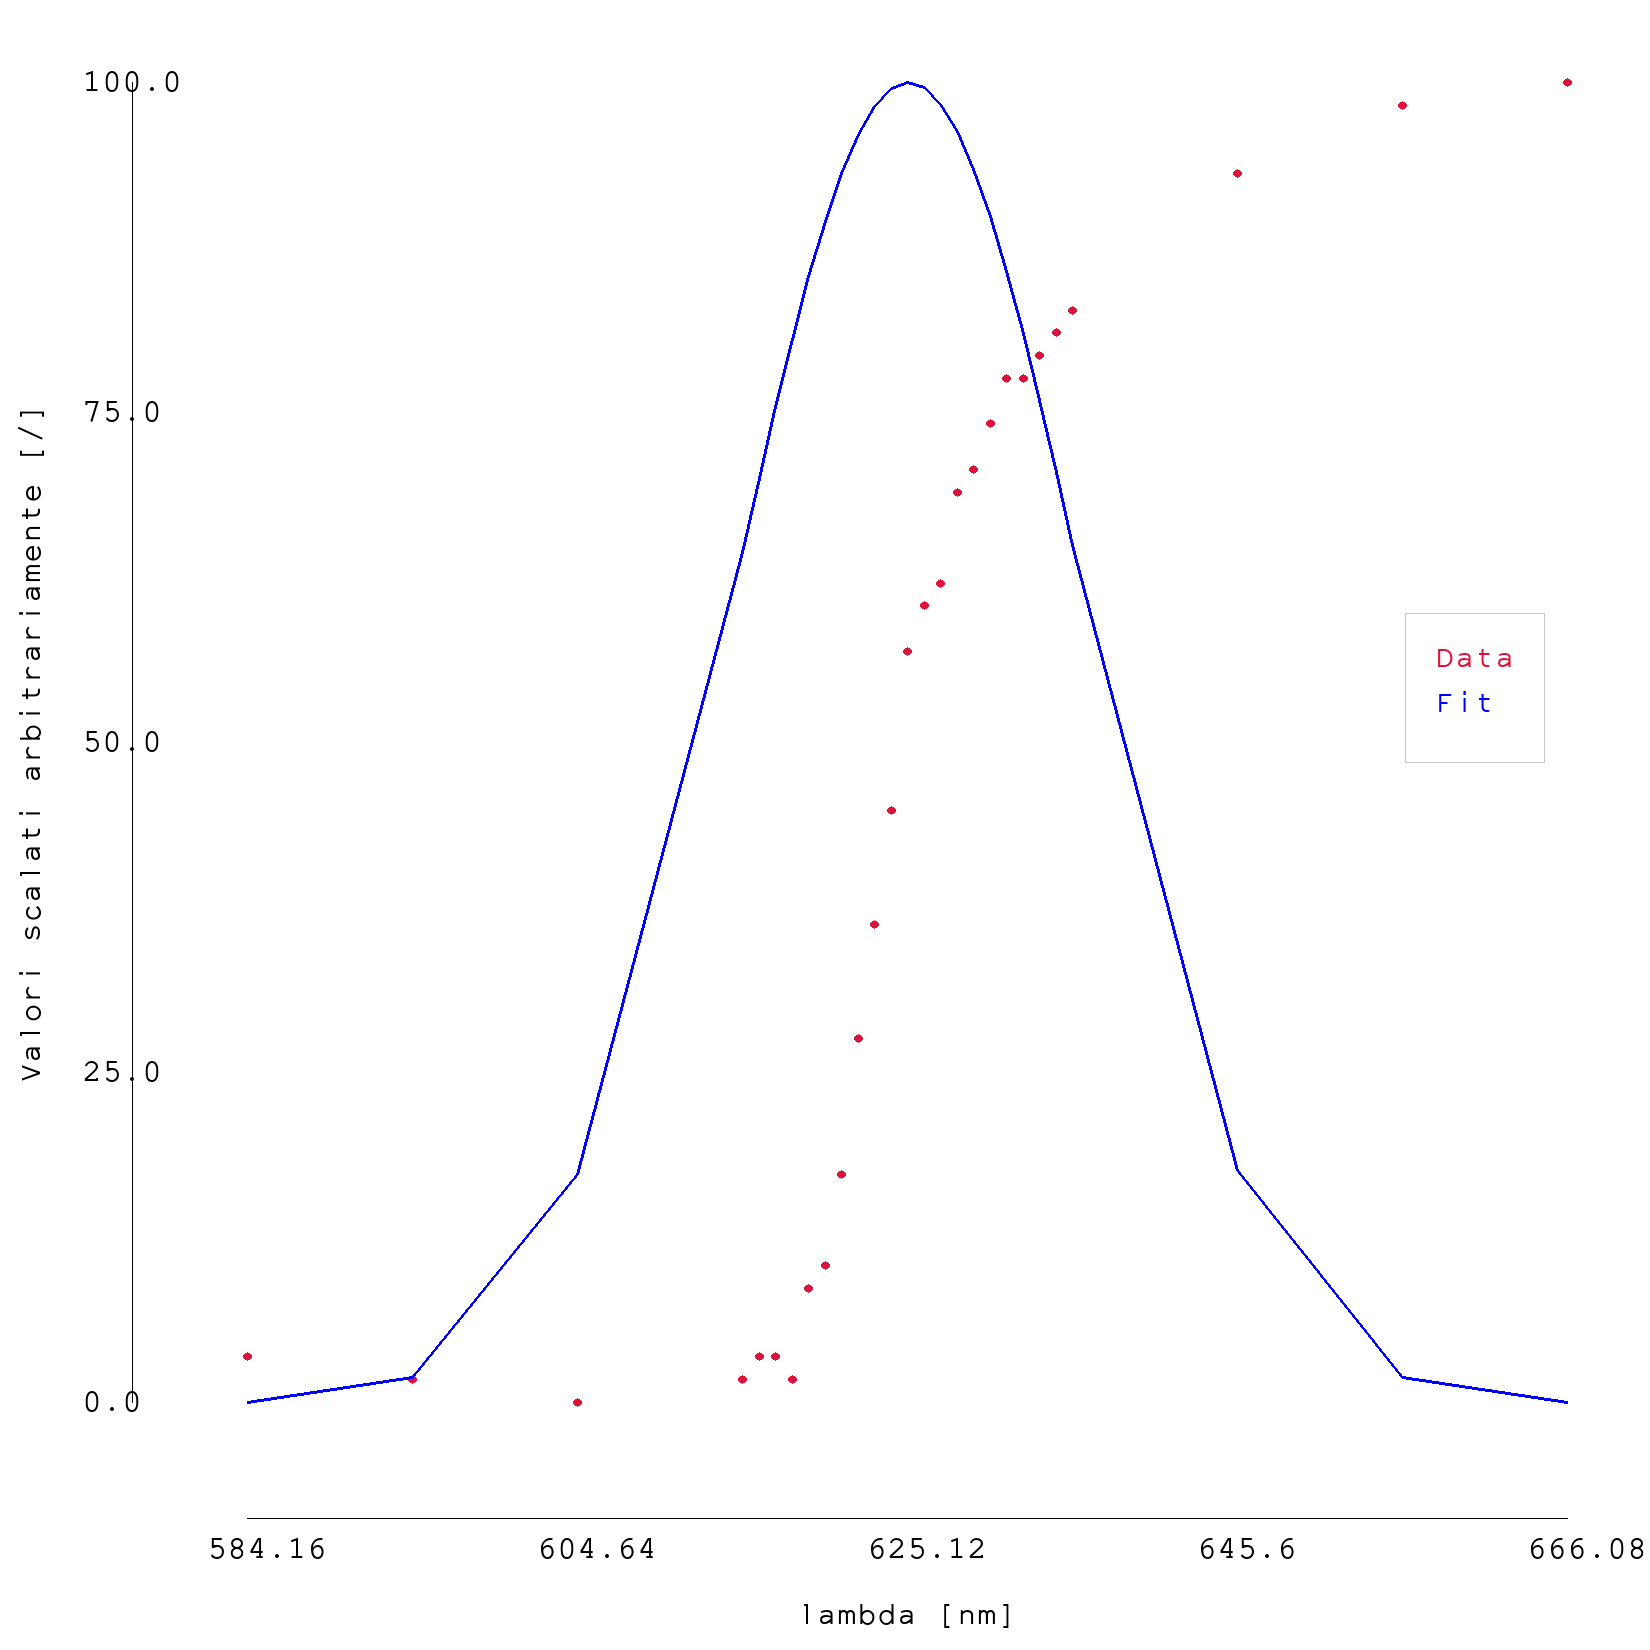
\includegraphics[width=1\linewidth]{../images/grafico3_1.png}
    \end{minipage}
    \hfill
    \begin{minipage}{0.25\textwidth}        
        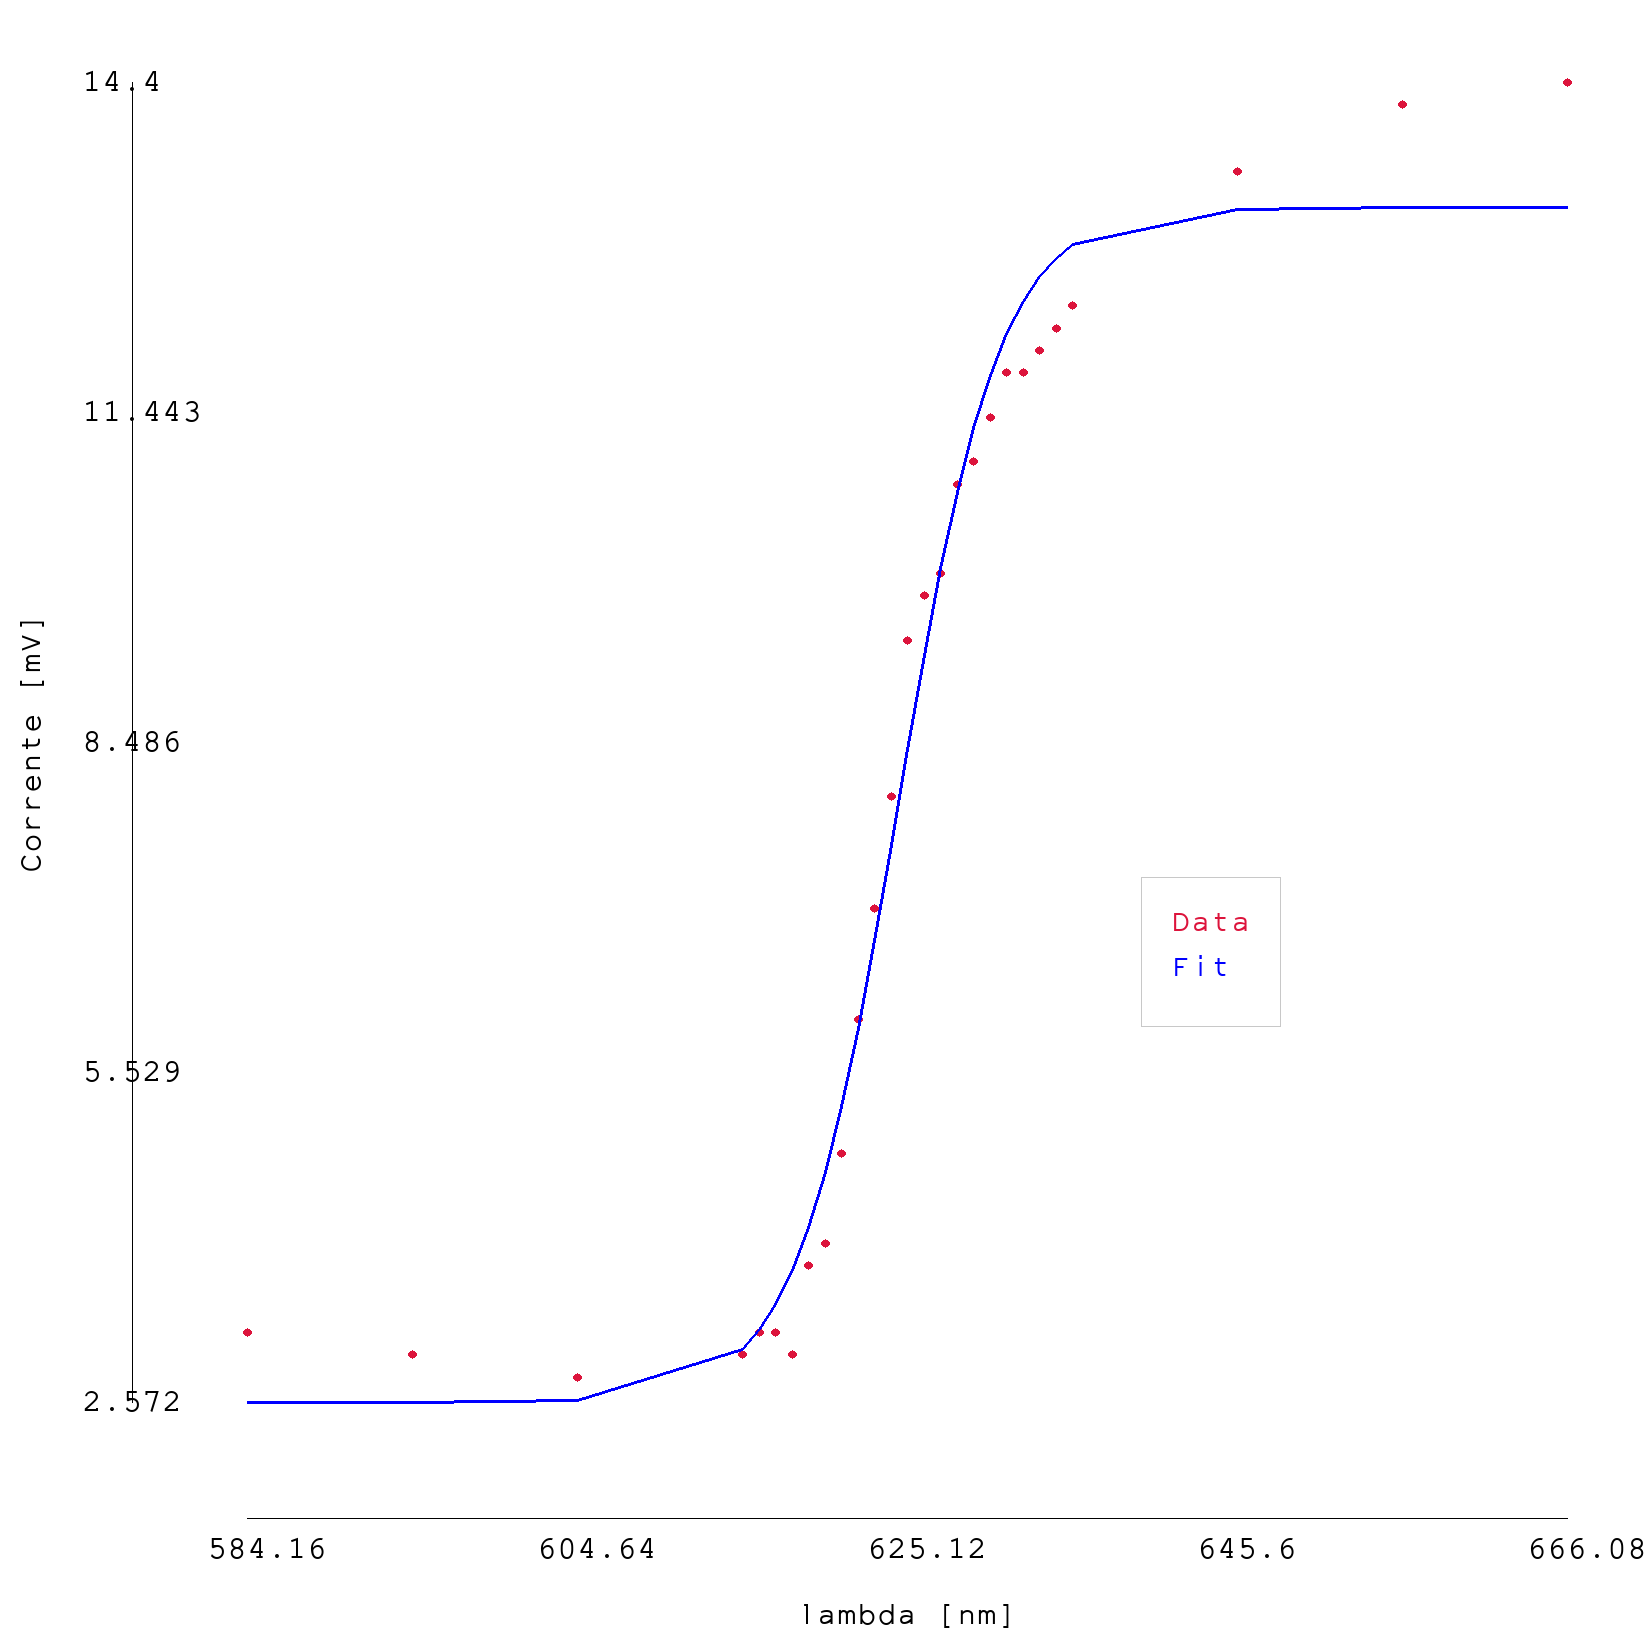
\includegraphics[width=1\linewidth]{../images/grafico2_1.png}
    \end{minipage}
    \captionof{figure}{Grafico del fit a) gaussiano con derivate, b) gaussiano con dati, c) sigmoide sul CH1 non normalizzato}
\end{center}

\begin{center}
    \begin{minipage}{0.25\textwidth}        
        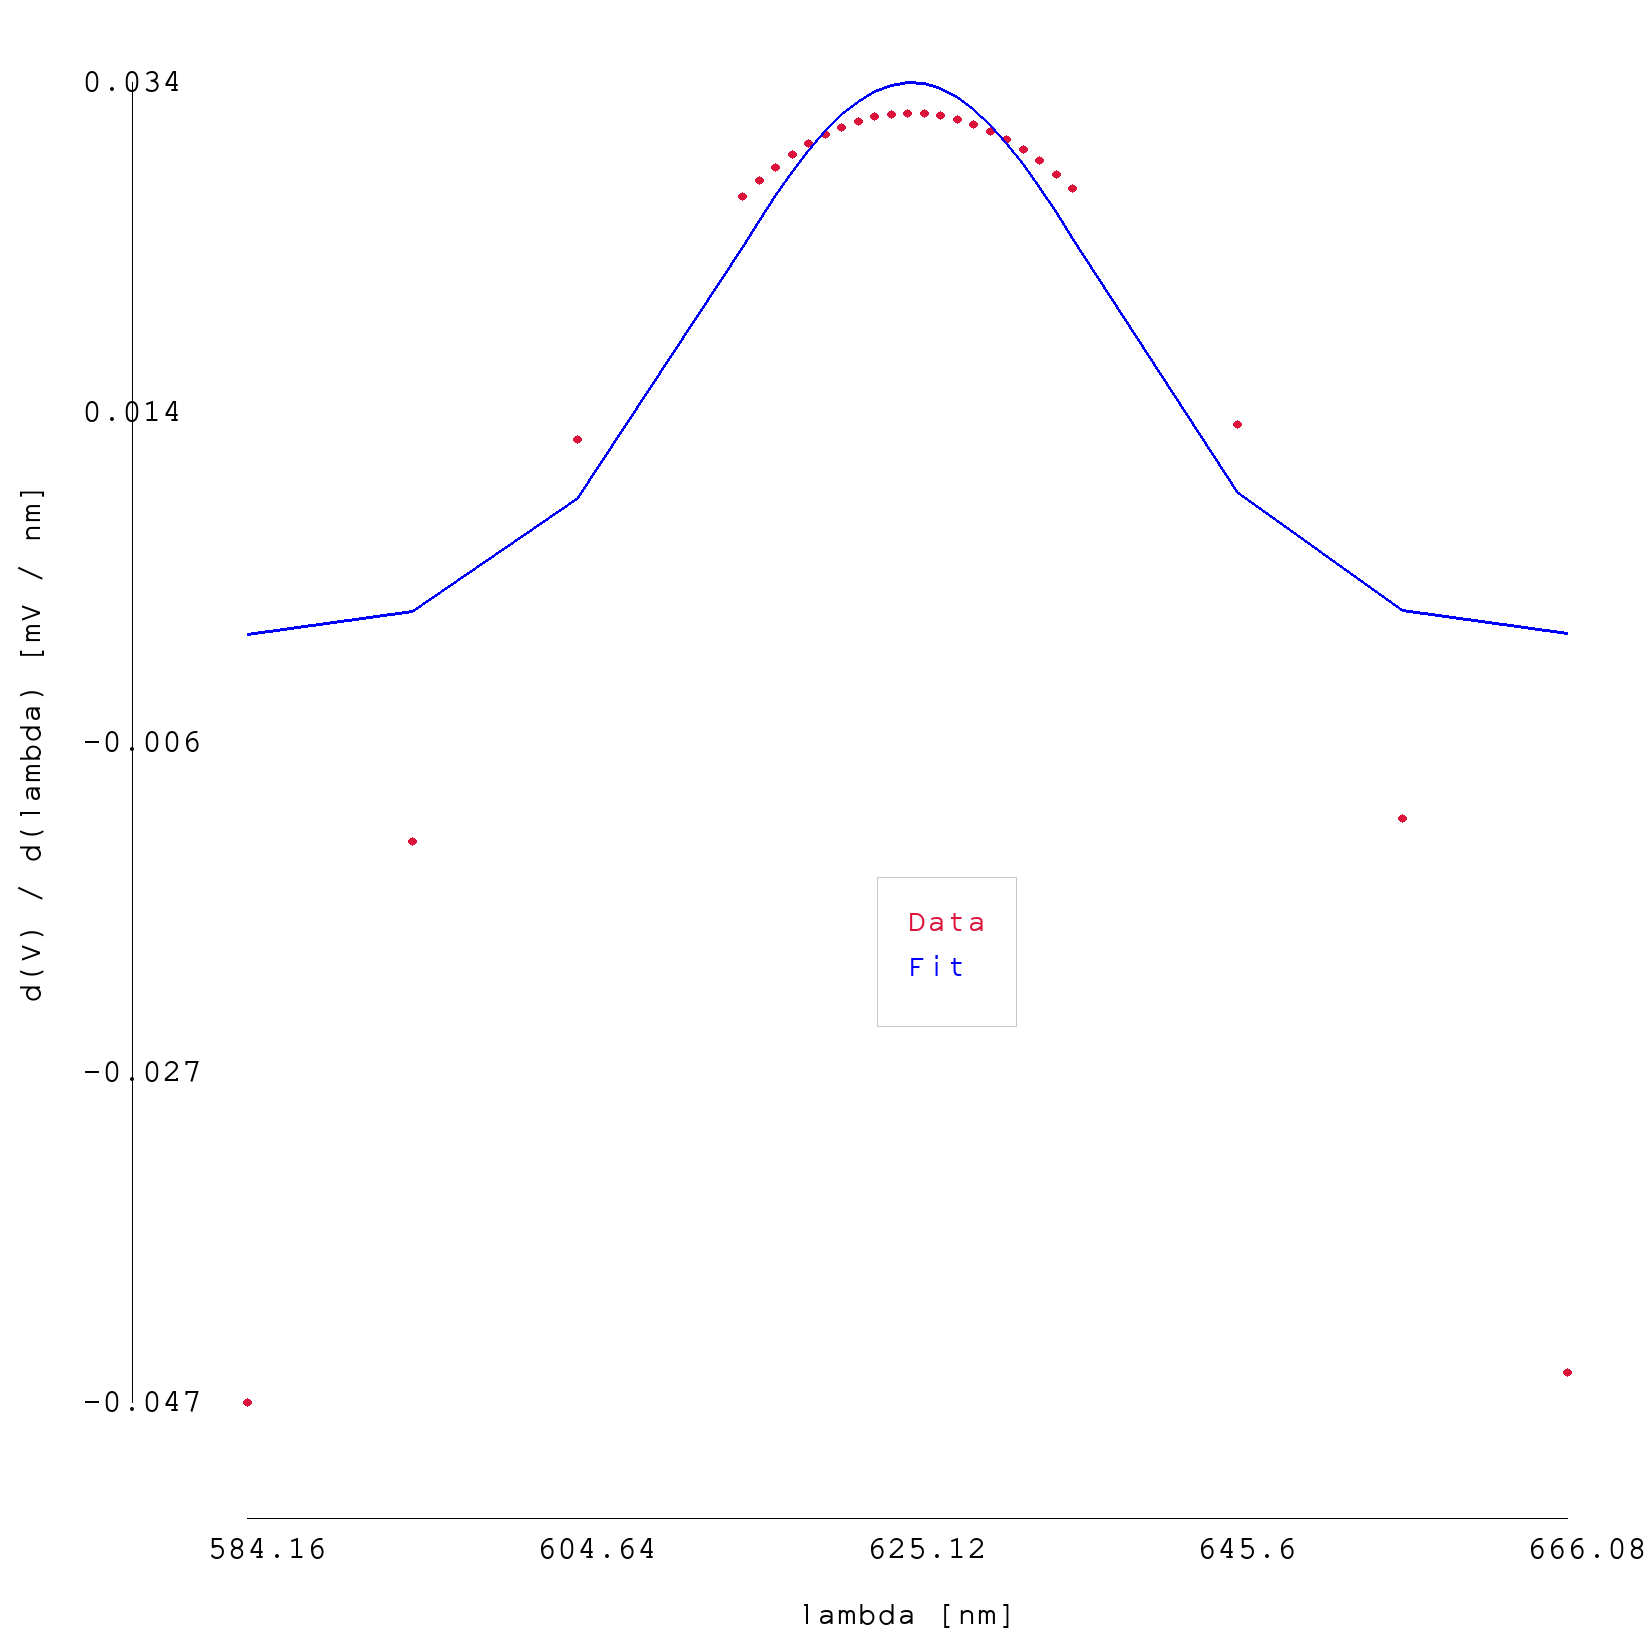
\includegraphics[width=1\linewidth]{../images/grafico1_2.png}
    \end{minipage}
    \hfill
    \begin{minipage}{0.25\textwidth}        
        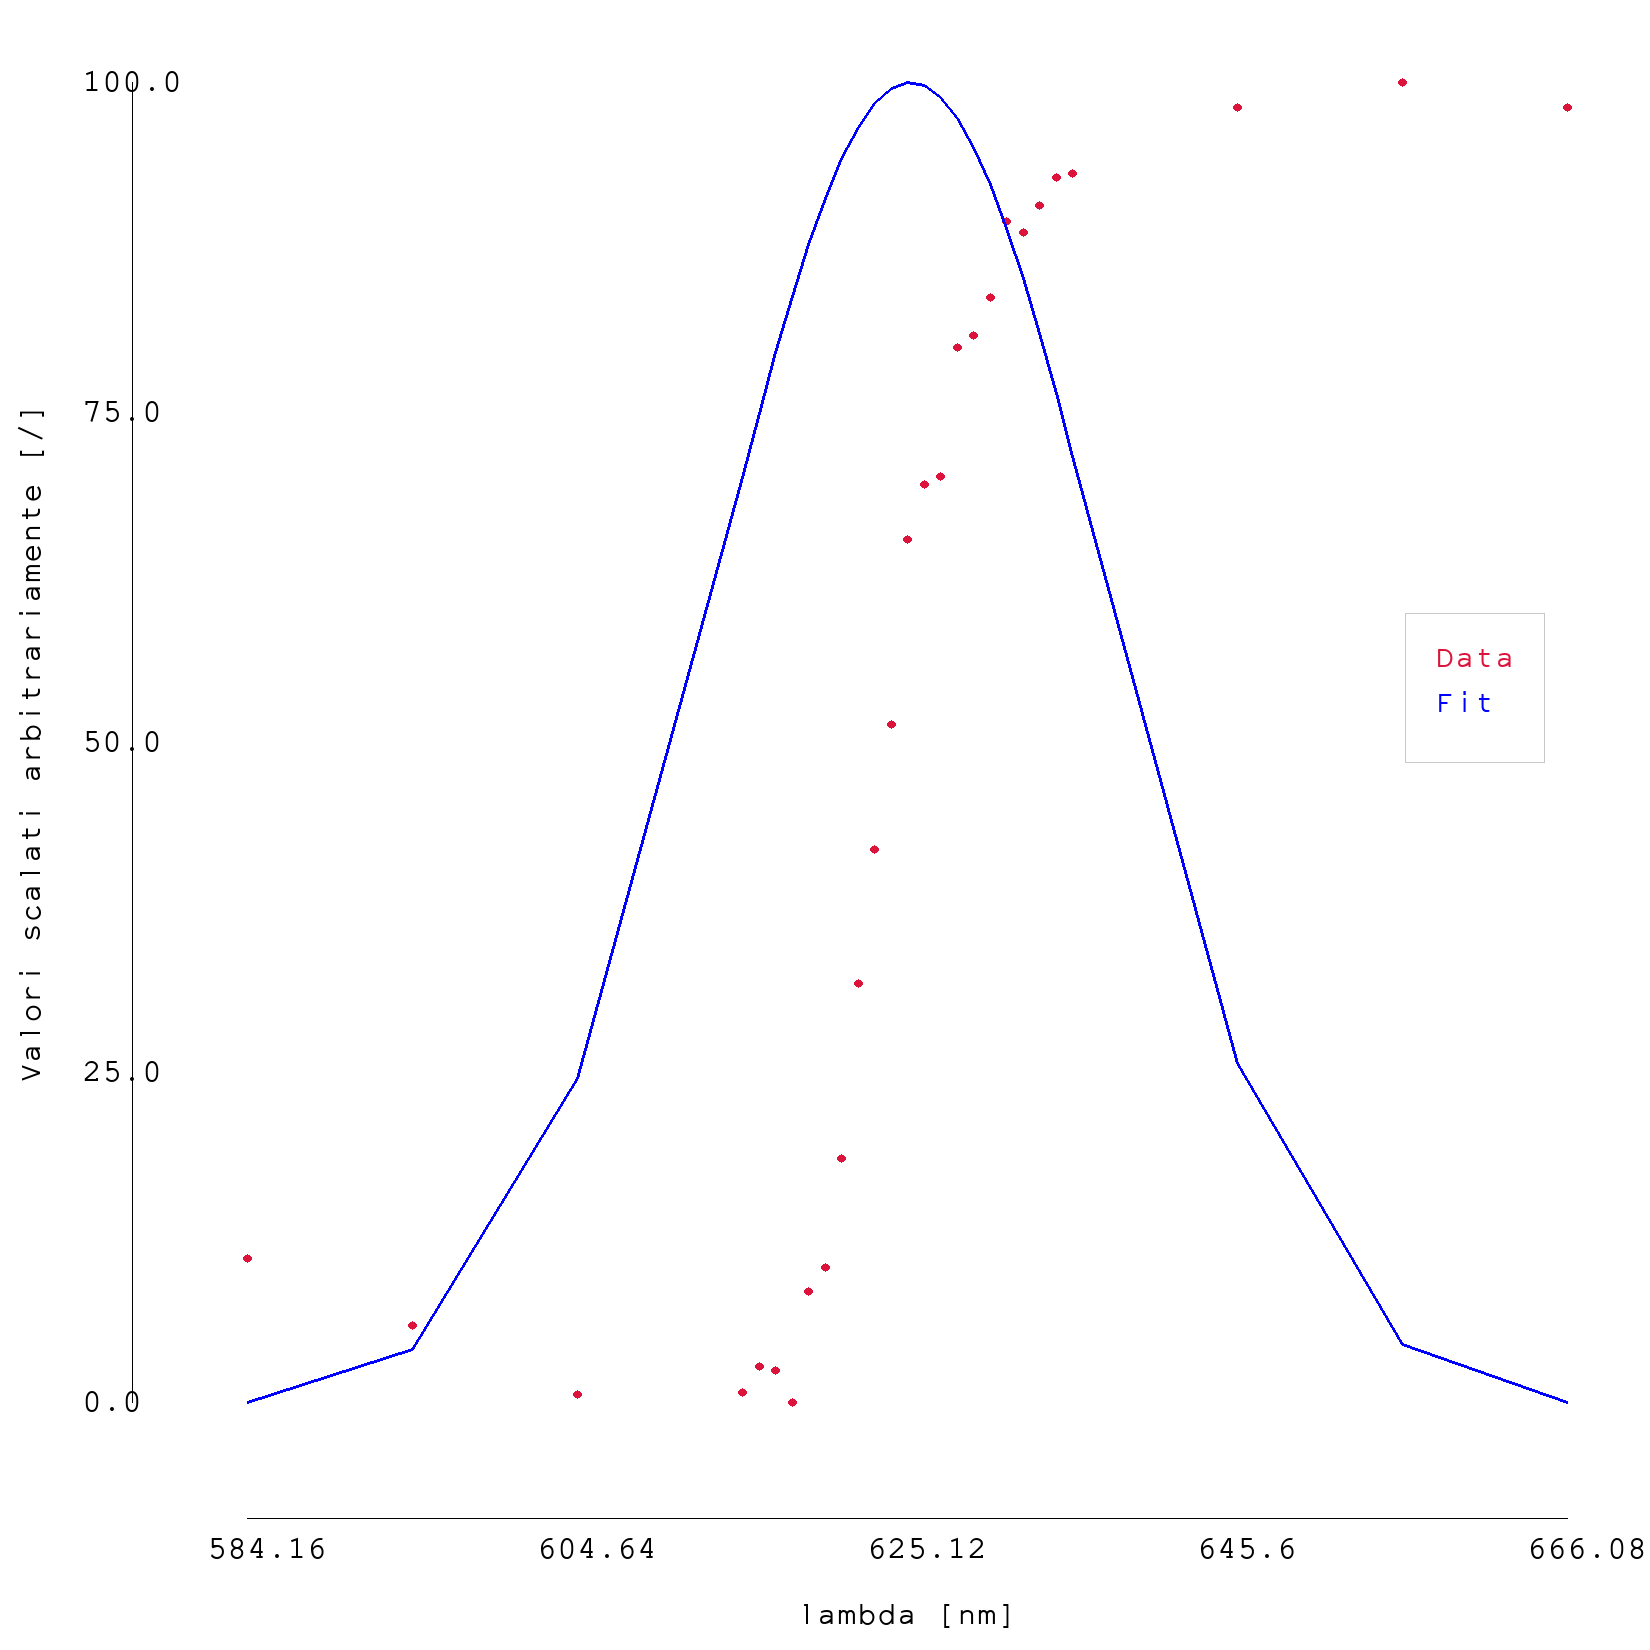
\includegraphics[width=1\linewidth]{../images/grafico3_2.png}
    \end{minipage}
    \hfill
    \begin{minipage}{0.25\textwidth}        
        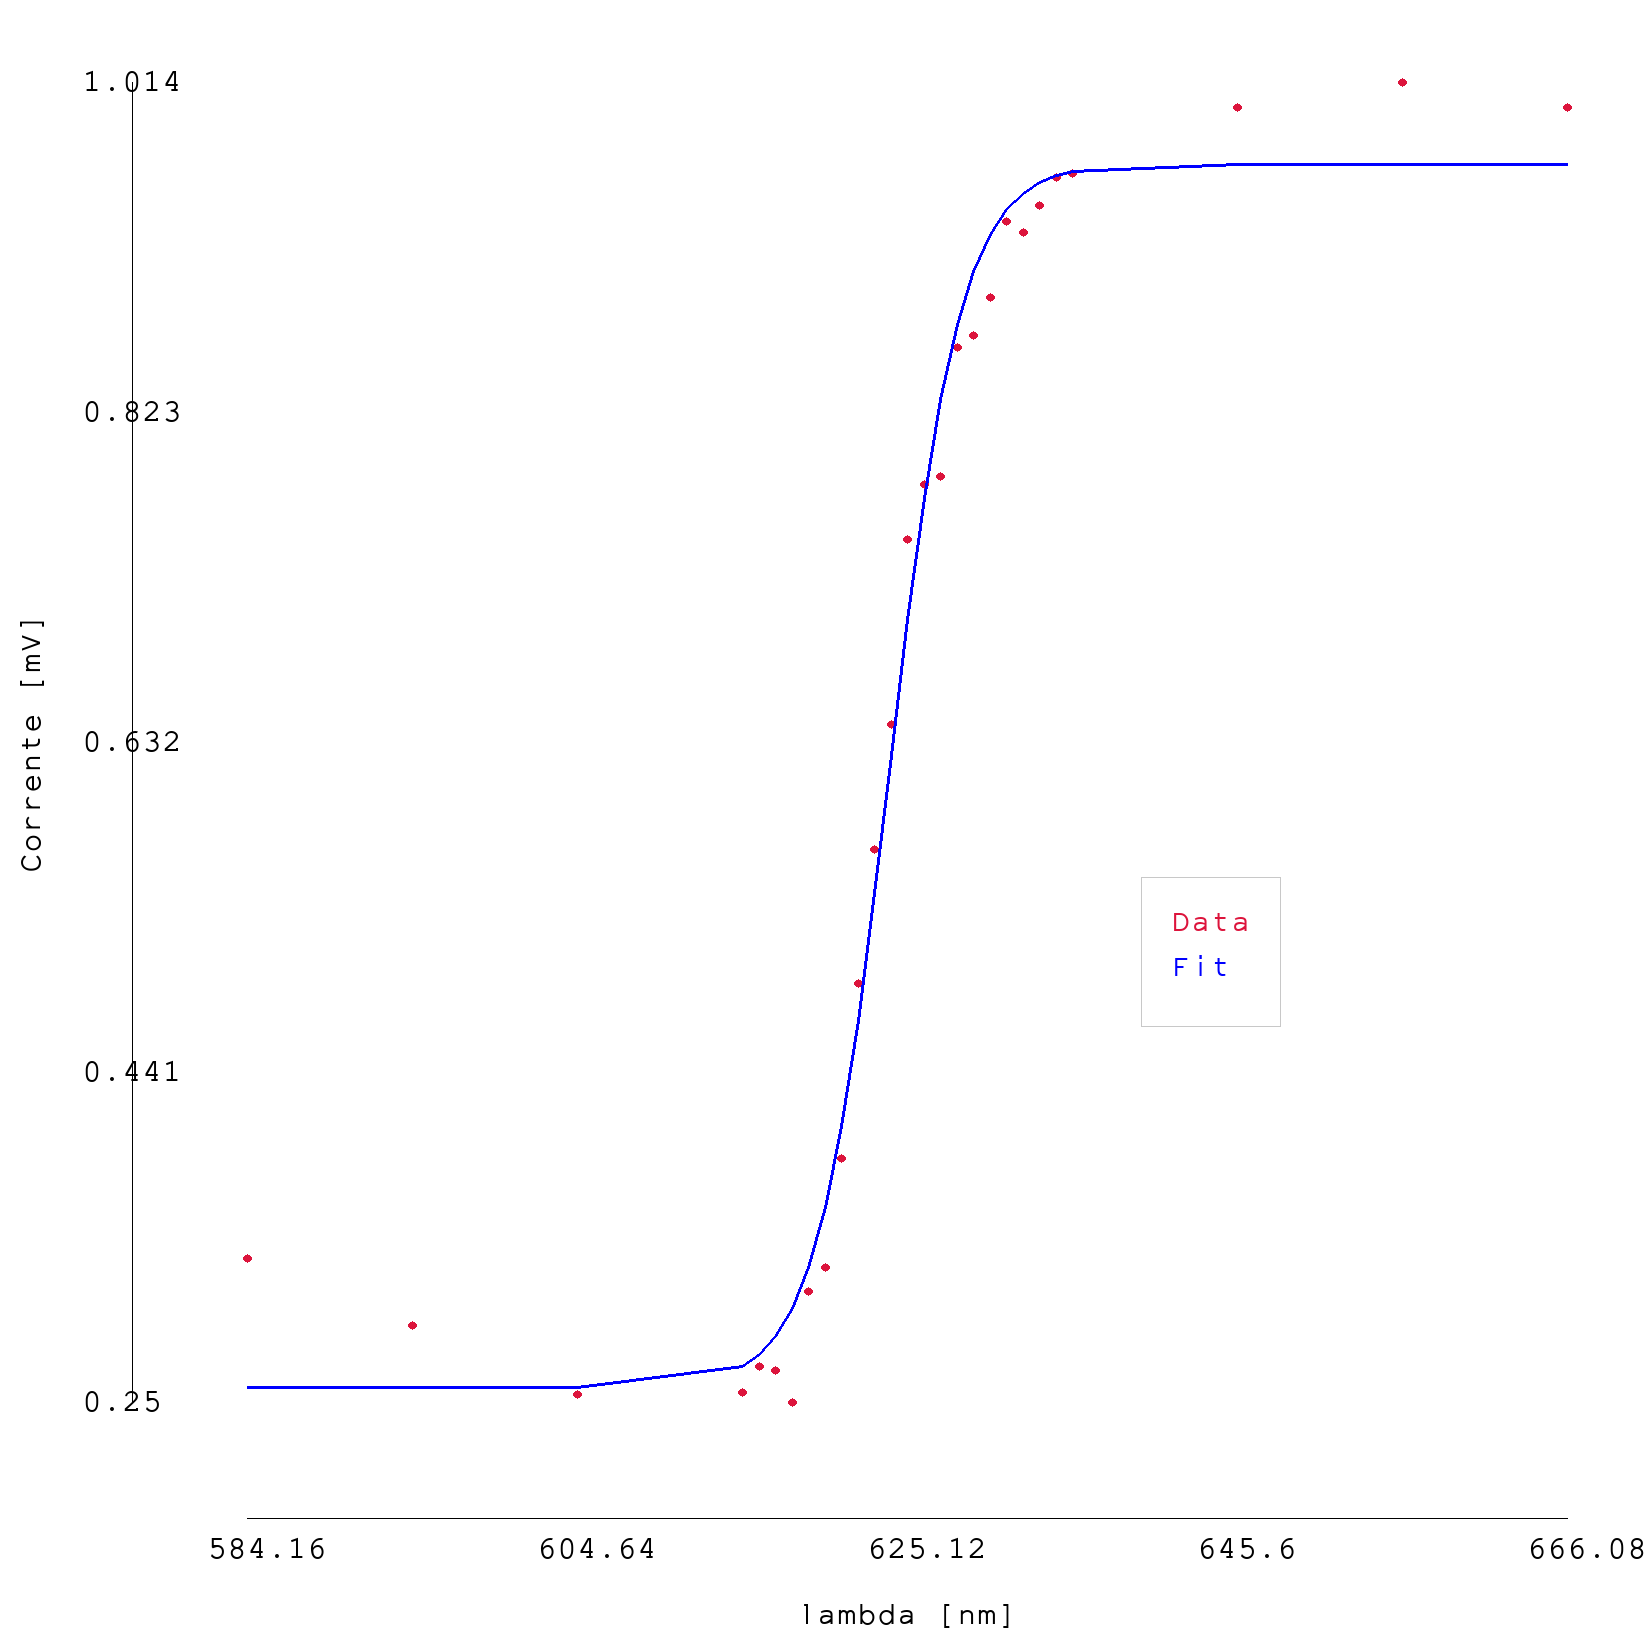
\includegraphics[width=1\linewidth]{../images/grafico2_2.png}
    \end{minipage}
    \captionof{figure}{Grafico del fit a) gaussiano con derivate, b) gaussiano con dati, c) sigmoide sul CH1 normalizzato}
\end{center}

\begin{center}
    \begin{minipage}{0.25\textwidth}        
        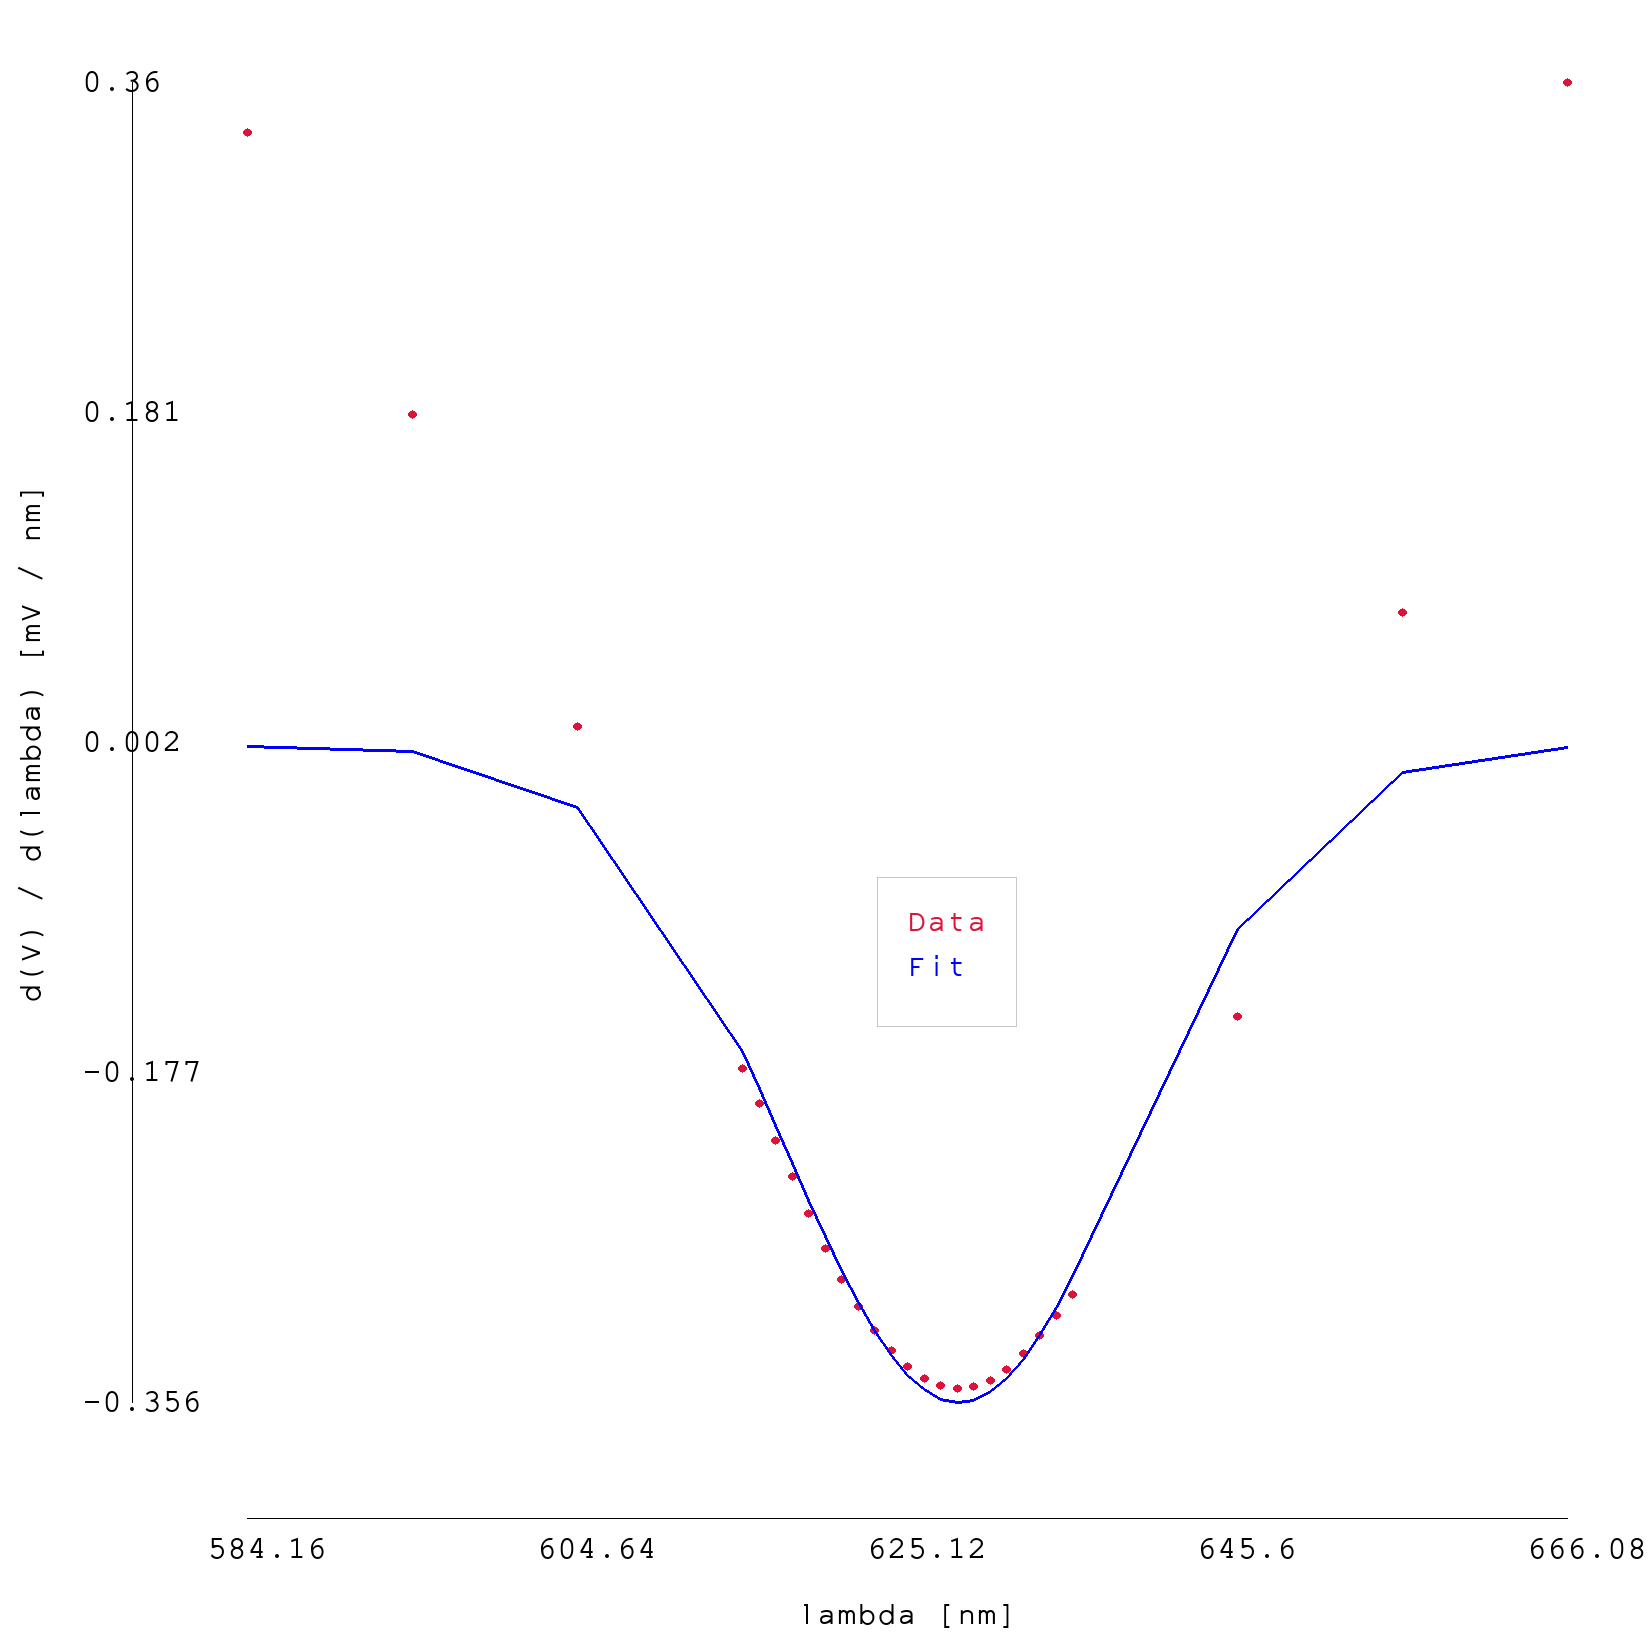
\includegraphics[width=1\linewidth]{../images/grafico1_3.png}
    \end{minipage}
    \hfill
    \begin{minipage}{0.25\textwidth}        
        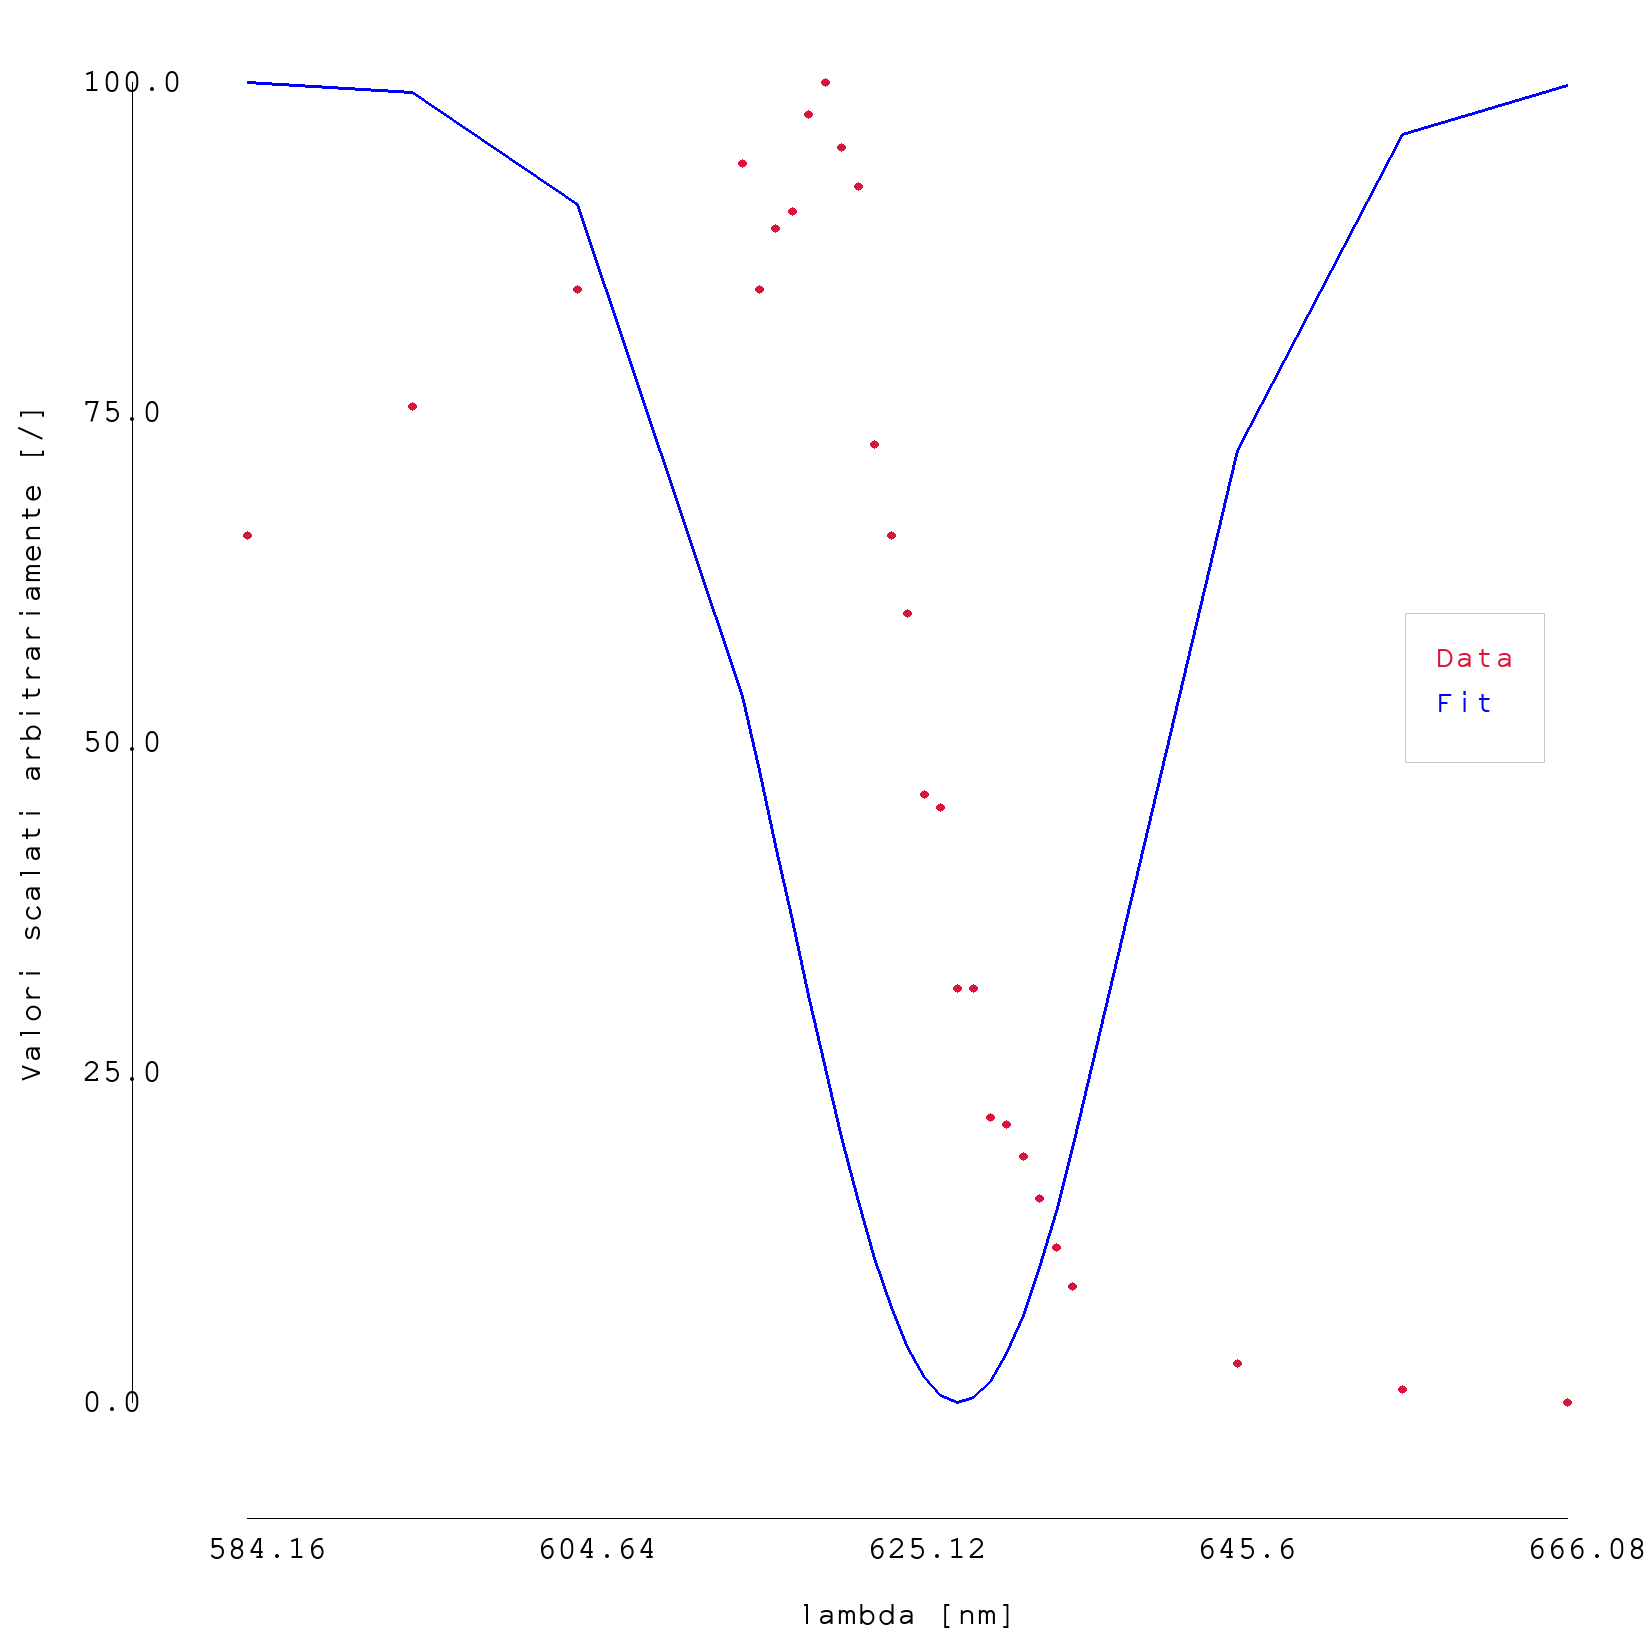
\includegraphics[width=1\linewidth]{../images/grafico3_3.png}
    \end{minipage}
    \hfill
    \begin{minipage}{0.25\textwidth}        
        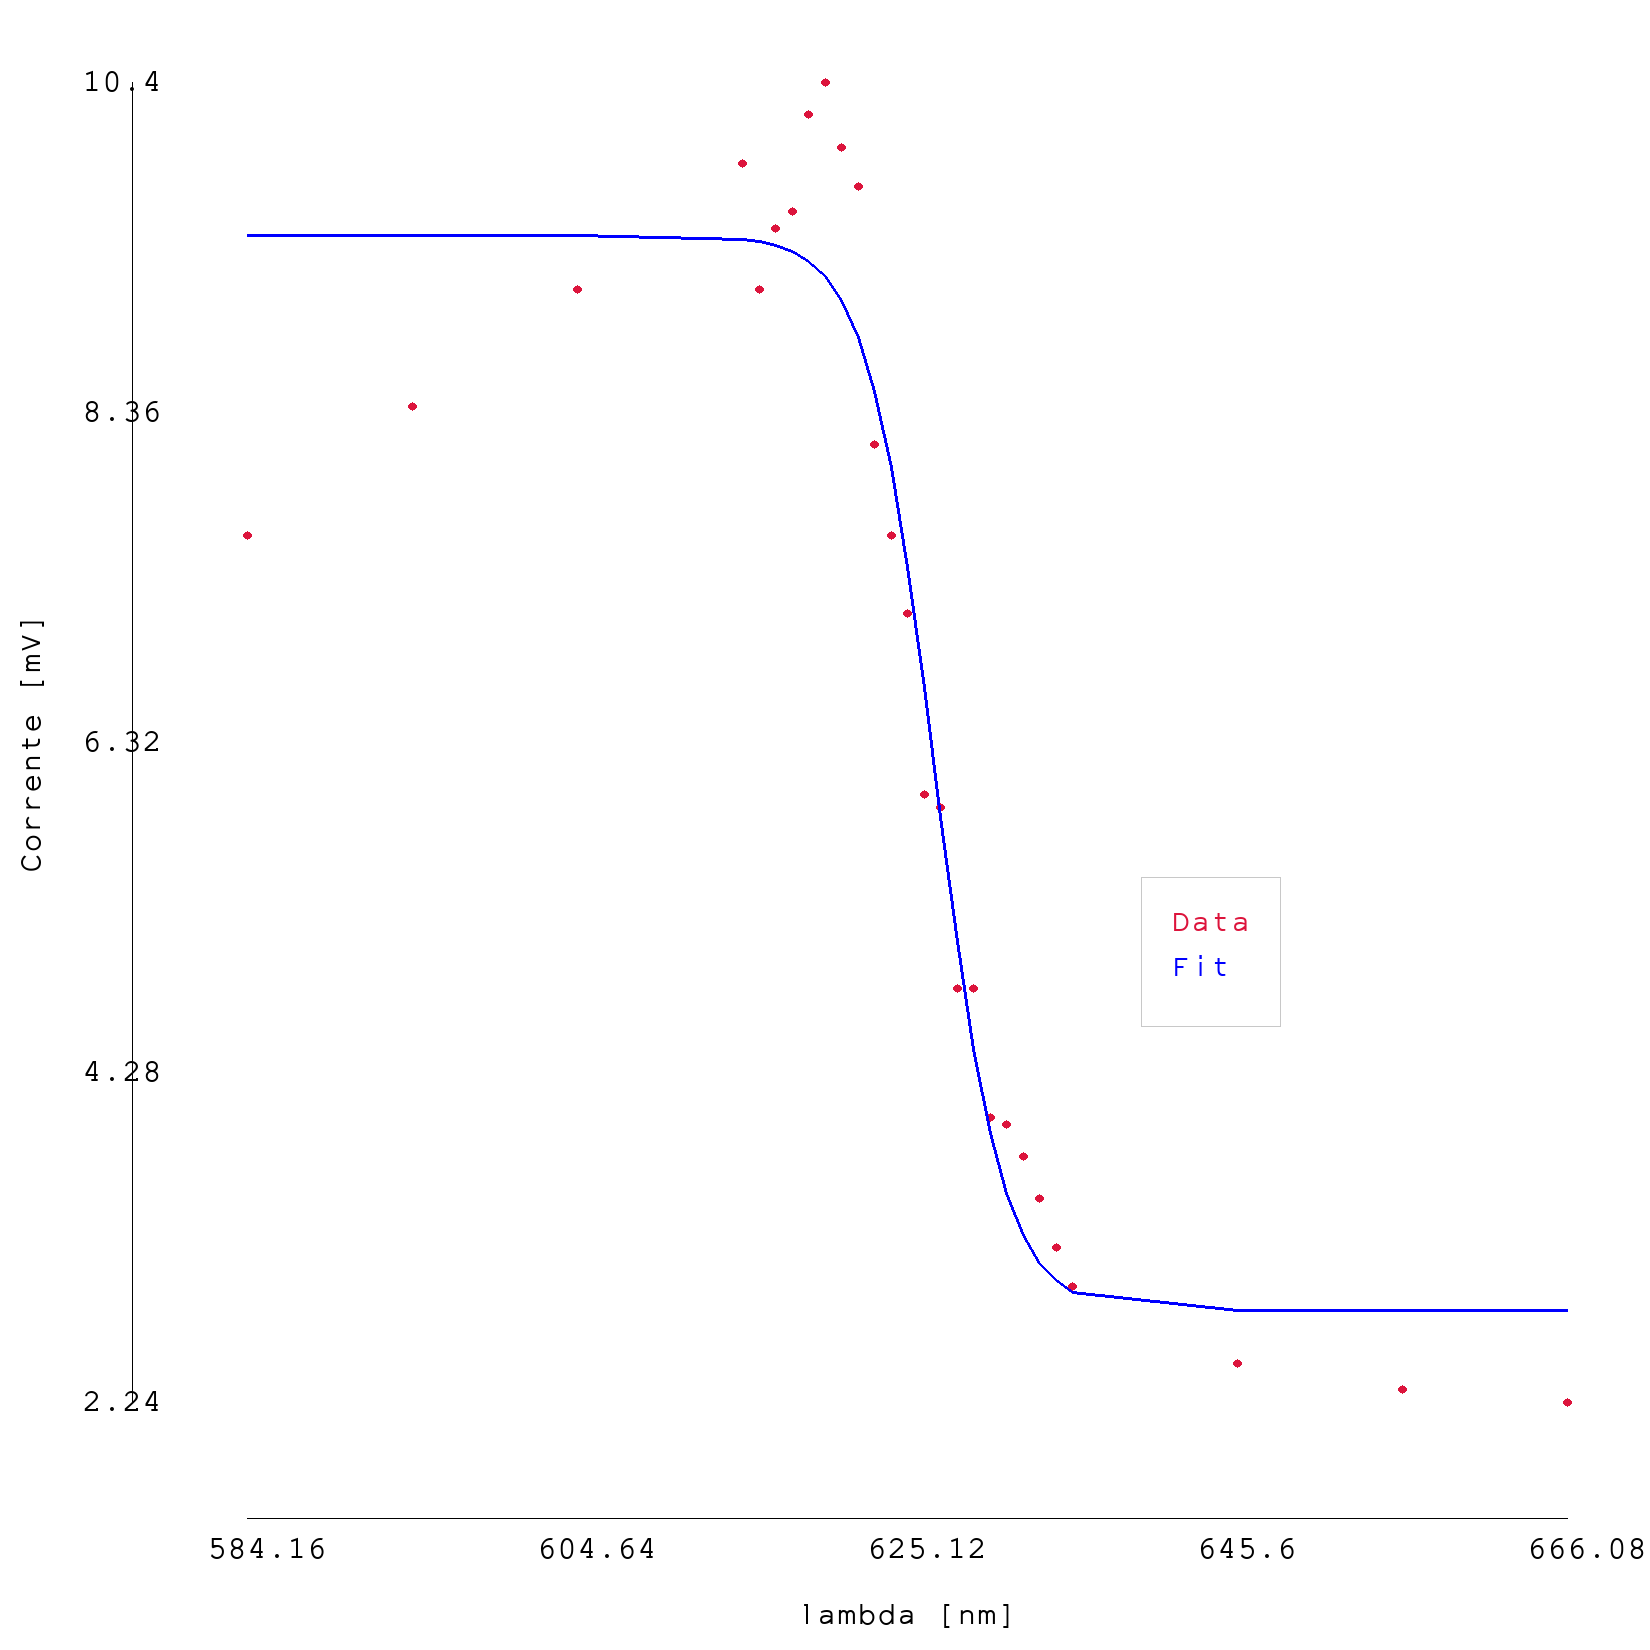
\includegraphics[width=1\linewidth]{../images/grafico2_3.png}
    \end{minipage}
    \captionof{figure}{Grafico del fit a) gaussiano con derivate, b) gaussiano con dati, c) sigmoide sul CH2 non normalizzato}
\end{center}

\begin{center}
    \begin{minipage}{0.25\textwidth}        
        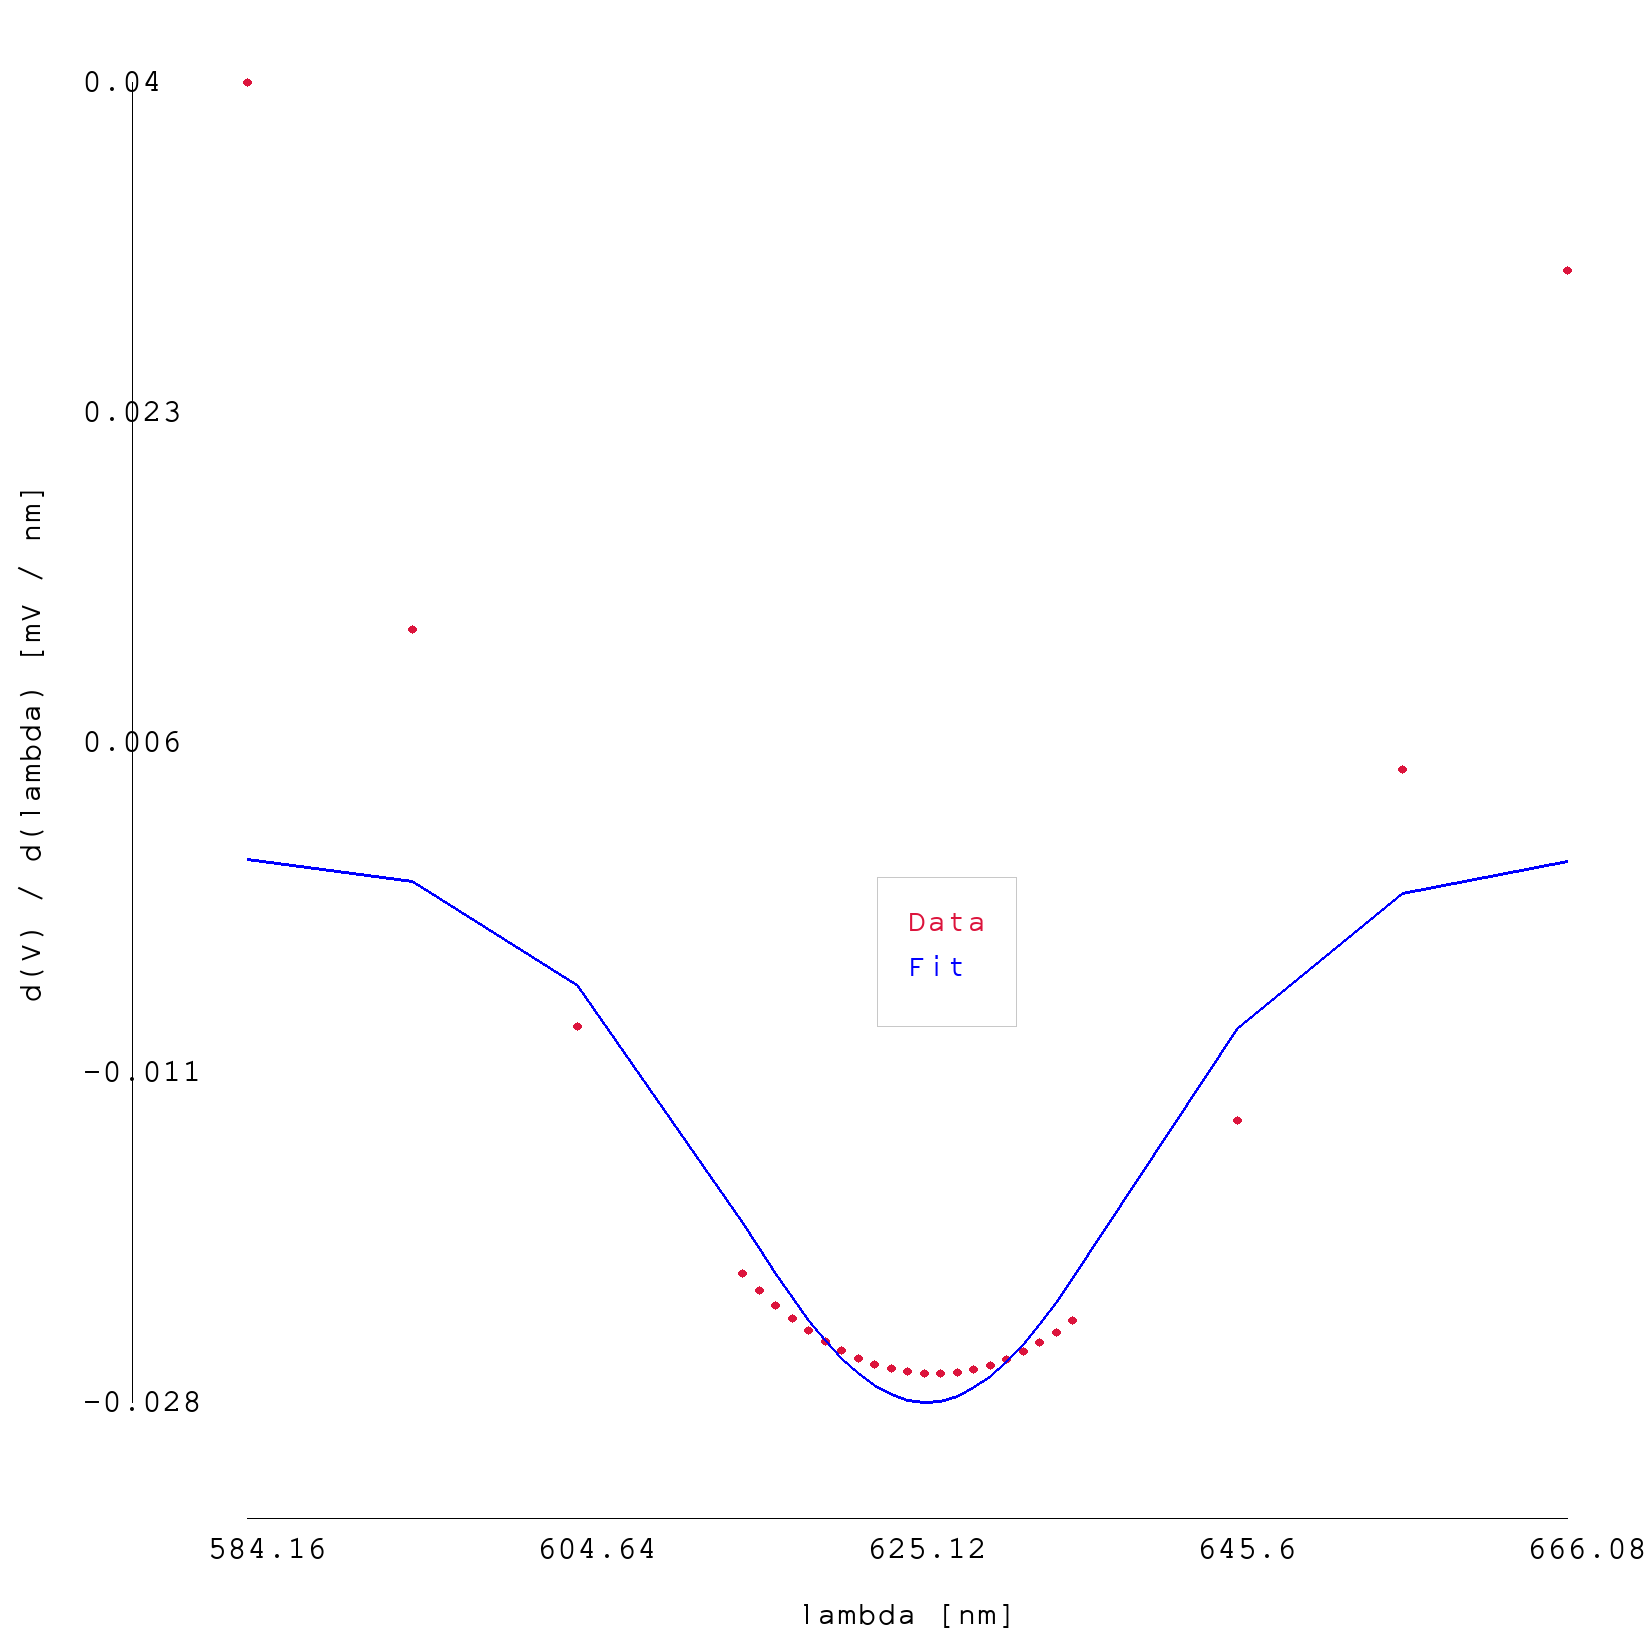
\includegraphics[width=1\linewidth]{../images/grafico1_4.png}
    \end{minipage}
    \hfill
    \begin{minipage}{0.25\textwidth}        
        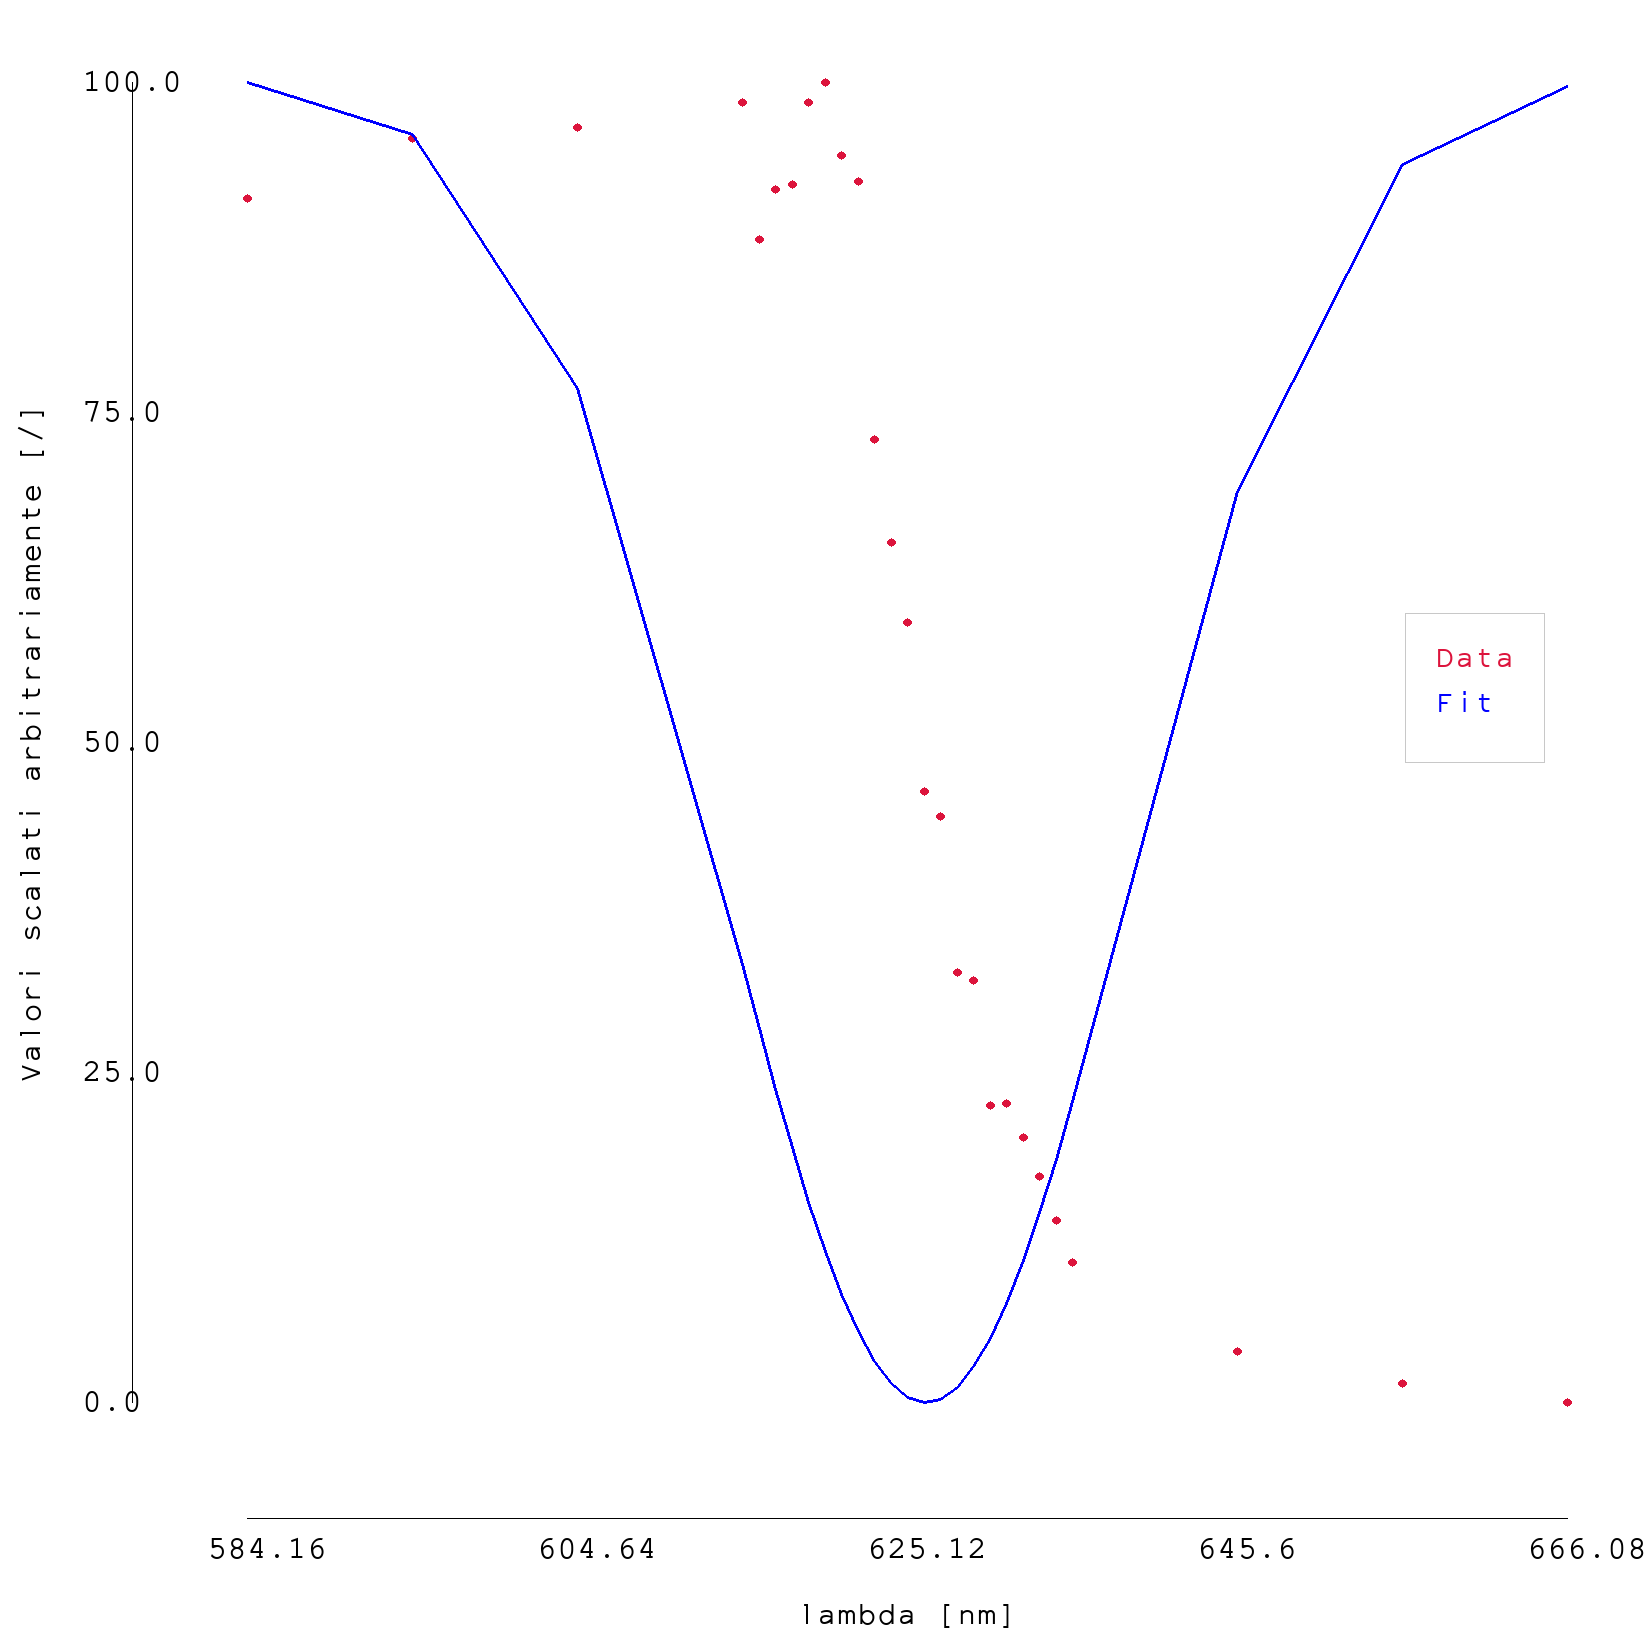
\includegraphics[width=1\linewidth]{../images/grafico3_4.png}
    \end{minipage}
    \hfill
    \begin{minipage}{0.25\textwidth}        
        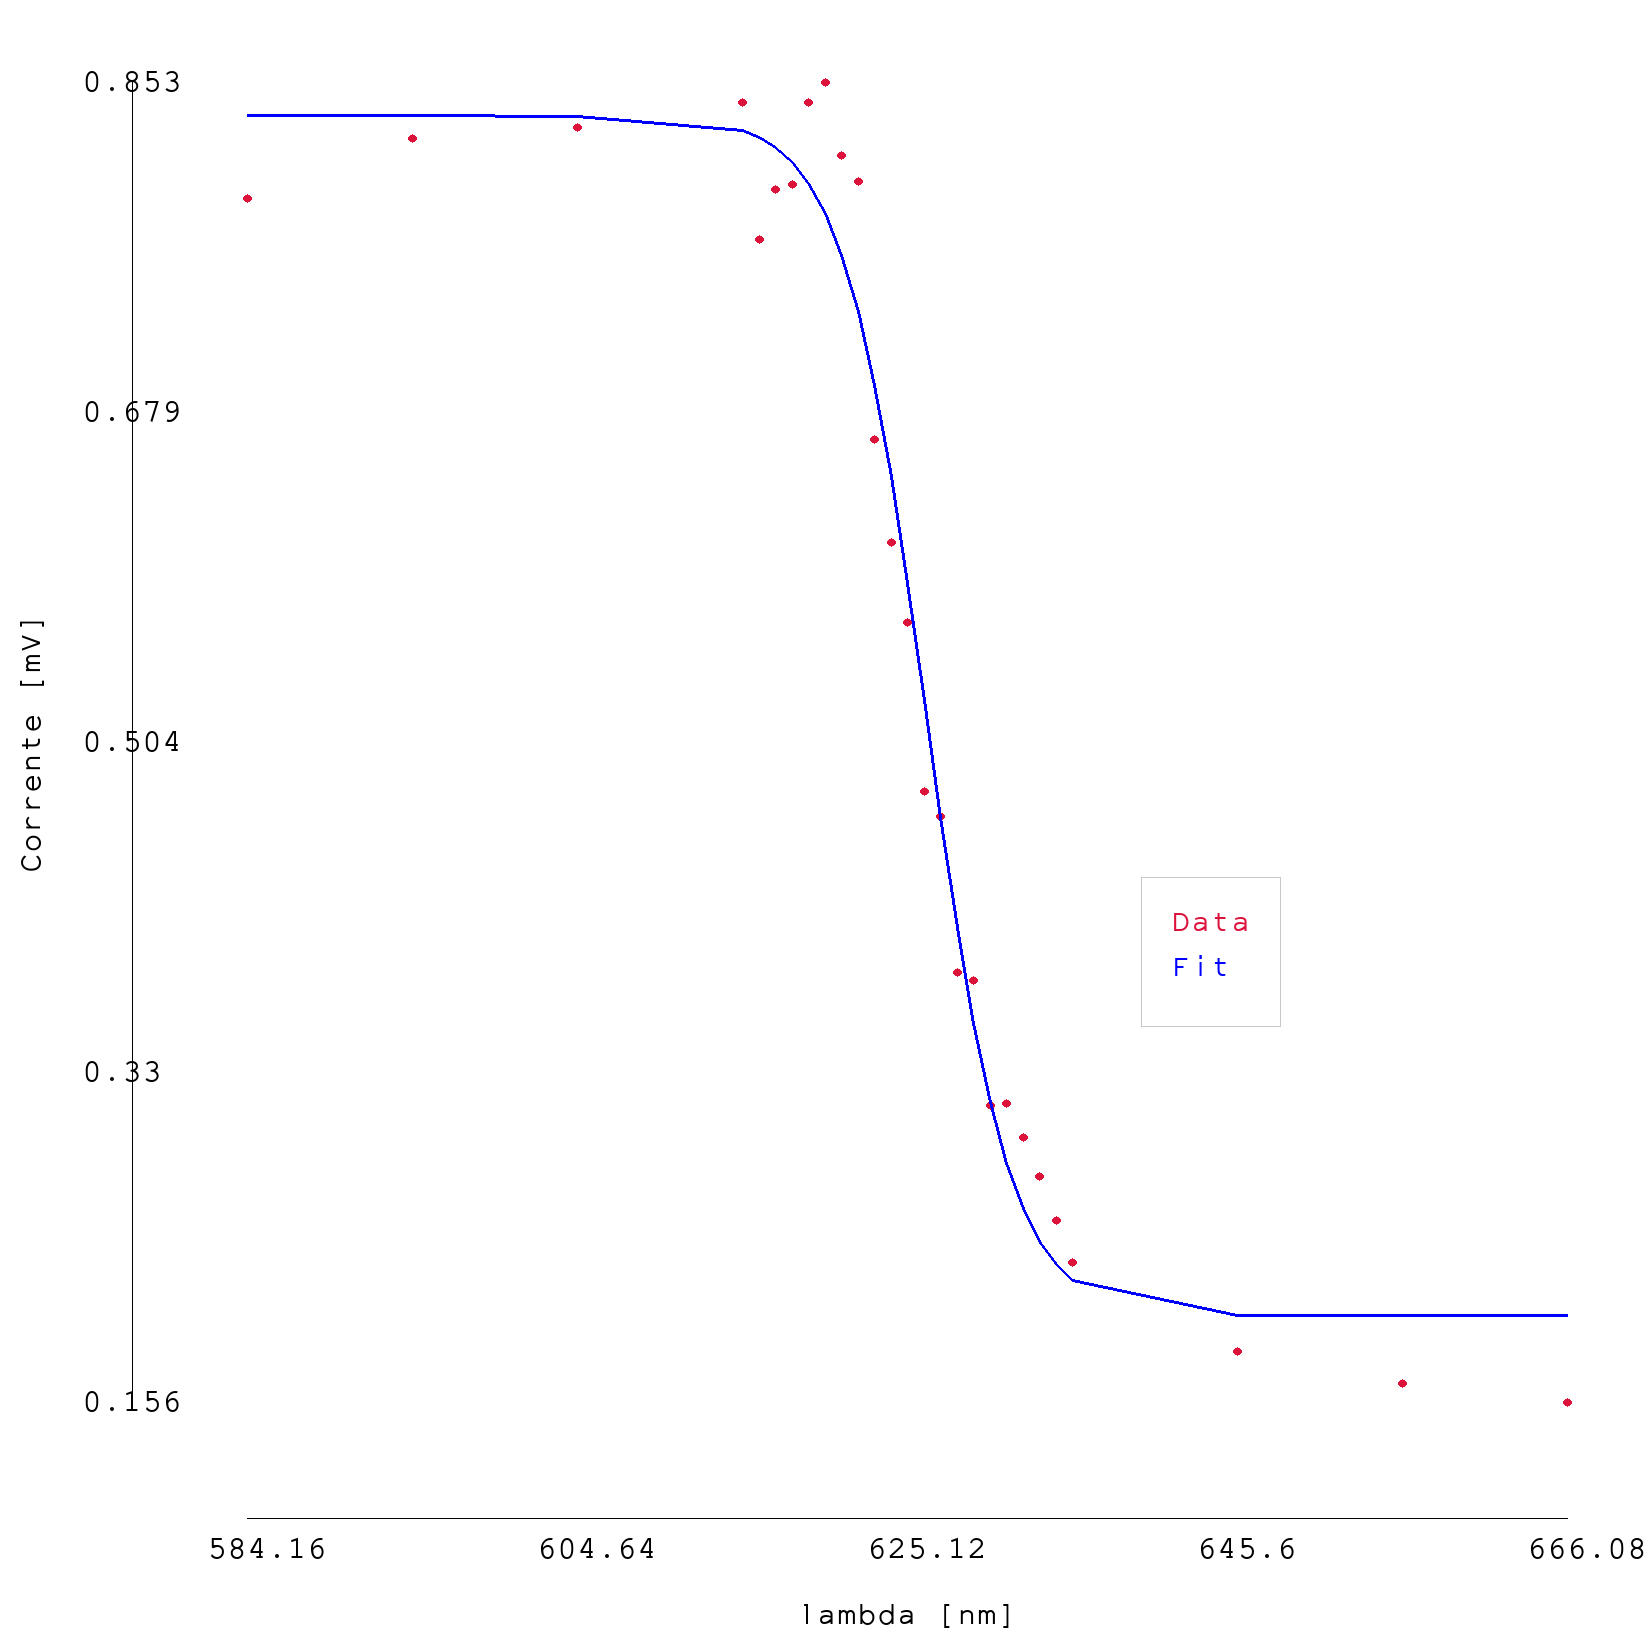
\includegraphics[width=1\linewidth]{../images/grafico2_4.png}
    \end{minipage}
    \captionof{figure}{Grafico del fit a) gaussiano con derivate, b) gaussiano con dati, c) sigmoide sul CH2 normalizzato}
\end{center}

\newpage

\section{Appendice}

\begin{table}[htbp]
    \centering
    \begin{tabular}{llll}
\toprule
tensione voltmetro [V] & I[mA] & errore V & errore I [mA] \\
\midrule
-30.05 & -3.04 & 0.08 & 0.04 \\
-27.01 & -2.73 & 0.08 & 0.04 \\
-24.08 & -2.43 & 0.07 & 0.03 \\
-21.05 & -2.12 & 0.07 & 0.03 \\
-18.05 & -1.82 & 0.07 & 0.03 \\
-15.03 & -1.52 & 0.07 & 0.03 \\
-10.08 & -1.02 & 0.06 & 0.03 \\
-6.01 & -0.60 & 0.06 & 0.02 \\
-3.00 & -0.30 & 0.05 & 0.02 \\
3.07 & 0.31 & 0.05 & 0.02 \\
6.01 & 0.60 & 0.06 & 0.02 \\
9.07 & 0.91 & 0.06 & 0.03 \\
12.08 & 1.22 & 0.06 & 0.03 \\
15.07 & 1.52 & 0.07 & 0.03 \\
18.03 & 1.82 & 0.07 & 0.03 \\
21.04 & 2.12 & 0.07 & 0.03 \\
24.01 & 2.43 & 0.07 & 0.03 \\
27.09 & 2.74 & 0.08 & 0.04 \\
30.06 & 3.04 & 0.08 & 0.04 \\
\bottomrule
\end{tabular}

    \caption{Dati caratterizzazione resistenza Ohmica}
    \label{tab:tabella1}
\end{table}

\begin{table}[htbp]
    \centering
    \begin{tabular}{rrrrrr}
\toprule
tensione [V] & corrente [$\mu$A] & Err V  & Err [$\mu$A] & corrente ln [$\mu$A] & Err [$\mu$A] \\
\midrule
0.0300 & 0.0036 & 0.0004 & 0.0001 & -5.626821 & 0.000018 \\
0.0700 & 0.0099 & 0.0008 & 0.0001 & -4.61522 & 0.00002 \\
0.090 & 0.015 & 0.001 & 0.001 & -4.2267 & 0.0002 \\
0.130 & 0.026 & 0.001 & 0.001 & -3.6497 & 0.0003 \\
0.160 & 0.043 & 0.002 & 0.001 & -3.1442 & 0.0003 \\
0.190 & 0.071 & 0.002 & 0.001 & -2.6451 & 0.0004 \\
0.210 & 0.106 & 0.002 & 0.001 & -2.2443 & 0.0004 \\
0.250 & 0.242 & 0.003 & 0.001 & -1.4188 & 0.0007 \\
0.300 & 0.830 & 0.003 & 0.001 & -0.186 & 0.005 \\
0.320 & 1.480 & 0.003 & 0.001 & 0.392 & 0.003 \\
0.370 & 4.911 & 0.004 & 0.001 & 1.5915 & 0.0006 \\
0.390 & 8.501 & 0.004 & 0.001 & 2.1402 & 0.0005 \\
0.430 & 24.711 & 0.004 & 0.001 & 3.2073 & 0.0003 \\
0.460 & 60.690 & 0.005 & 0.001 & 4.1058 & 0.0002 \\
0.490 & 100 & 0.005 & 1 & 4.6 & 0.2 \\
0.520 & 201 & 0.005 & 1 & 5.30 & 0.19 \\
0.550 & 390 & 0.006 & 1 & 5.97 & 0.17 \\
0.570 & 593 & 0.006 & 1 & 6.38 & 0.16 \\
0.600 & 1149 & 0.006 & 1 & 7.05 & 0.14 \\
\bottomrule
\end{tabular}

    \caption{Dati caratterizzazione tensione corrente in polarizzazione diretta}
    \label{tab:tabella2}
\end{table}

% \begin{table}[htbp]
%     \centering
%     \begin{tabular}{rrr}
\toprule
corrente ln [$\mu$A] & Err [$\mu$A] \\
\midrule
-5.626821 & 0.000018 \\
-4.6152 & 0.0002 \\
-4.2267 & 0.0002 \\
-3.6497 & 0.0003 \\
-3.1442 & 0.0003 \\
-2.6451 & 0.0004 \\
-2.2443 & 0.0004 \\
-1.4188 & 0.0007 \\
-0.186 & 0.005 \\
0.392 & 0.003 \\
1.5915 & 0.0006 \\
2.1402 & 0.0005 \\
3.2072 & 0.0003 \\
4.1058 & 0.0002 \\
4.6072 & 0.0002 \\
5.30330 & 0.00019 \\
5.96512 & 0.00017 \\
6.38469 & 0.00016 \\
7.04673 & 0.00014 \\
\bottomrule
\end{tabular}

%     \caption{Dati in scala logaritmica della polarizzazione diretta}
%     \label{tab:tabella3}
% \end{table}

\begin{table}[htbp]
    \centering
    \begin{tabular}{llll}
\toprule
tensione [V] & Err tensione generatore [V] & corrente [$\mu$A] & Errore corrente [$\mu$A] \\
\midrule
1.0 & 0.1 & 0.0008 & 0.0001 \\
2.5 & 0.1 & 0.0010 & 0.0001 \\
5.0 & 0.1 & 0.0013 & 0.0001 \\
7.5 & 0.1 & 0.0014 & 0.0001 \\
10.0 & 0.1 & 0.0015 & 0.0001 \\
12.5 & 0.1 & 0.0016 & 0.0001 \\
15.0 & 0.1 & 0.0017 & 0.0001 \\
17.5 & 0.1 & 0.0018 & 0.0001 \\
20.0 & 0.1 & 0.0019 & 0.0001 \\
22.5 & 0.1 & 0.0019 & 0.0001 \\
25.0 & 0.1 & 0.0020 & 0.0001 \\
27.5 & 0.1 & 0.0021 & 0.0001 \\
30.0 & 0.1 & 0.0021 & 0.0001 \\
31.8 & 0.1 & 0.0022 & 0.0001 \\
\bottomrule
\end{tabular}

    \caption{Dati corrente caratteristica polarizzazione inversa (per effettuare l'interpolazione non abbiamo utilizzato gli arrotondamenti per evitare di avere dati approssimati allo stesso valore nella prima metà del grafico)}
    \label{tab:tabella4}
\end{table}

\begin{table}[htbp]
    \centering
    \begin{tabular}{rrrrrrrrrr}
\toprule
voltm. $V_D$ $[V]$ & e. $V_D$ $[V]$ & $V_in$ $[V]$ & e. $V_in$ $[V]$ & $I [mA]$  & e. $I [mA]$ &  $ln(I)$ $[mA]$ & e. $ln(I)$ $[mA]$ & $I_L[a.u.]$ & e. $I[a.u]$ \\
\midrule
1.711 & 0.001 & 3.0 & 0.1 & -1.47 & 0.03 & 0.39 & 0.07 & 56800 & 200 \\
1.738 & 0.001 & 4.0 & 0.1 & -2.31 & 0.03 & 0.84 & 0.04 & 138500 & 400 \\
1.762 & 0.001 & 5.0 & 0.1 & -3.32 & 0.04 & 1.20 & 0.03 & 23400 & 500 \\
1.781 & 0.001 & 6.0 & 0.1 & -4.29 & 0.05 & 1.46 & 0.03 & 352500 & 600 \\
1.804 & 0.001 & 7.5 & 0.1 & -5.76 & 0.05 & 1.75 & 0.03 & 410000 & 600 \\
1.826 & 0.001 & 9.0 & 0.1 & -7.24 & 0.06 & 1.98 & 0.03 & 412300 & 600 \\
1.863 & 0.001 & 12.0 & 0.1 & -10.22 & 0.08 & 2.32 & 0.03 & 416000 & 600 \\
1.895 & 0.001 & 15.0 & 0.1 & -13.19 & 0.10 & 2.58 & 0.04 & 419000 & 600 \\
1.926 & 0.001 & 18.0 & 0.1 & -16.25 & 0.12 & 2.79 & 0.04 & 421000 & 600 \\
1.954 & 0.001 & 21.0 & 0.1 & -19.33 & 0.14 & 2.96 & 0.05 & 423500 & 700 \\
\bottomrule
\end{tabular}





    \caption{Caratterizzazione LED}
    \label{tab:tabella5}
\end{table}

\begin{table}[htbp]
    \centering
    \begin{tabular}{rrrrrr}
\toprule
UA & pixel & FWHM (pixel) & err. \% (pixel) & $\lambda [nm]$ & err. $\lambda [nm]$ \\
\midrule
500 & 735 & 42 & 6 & 495 & 28 \\
525 & 861 & 45 & 5 & 520 & 27 \\
550 & 980 & 45 & 5 & 544 & 25 \\
575 & 1104 & 45 & 4 & 569 & 23 \\
600 & 1232 & 43 & 3 & 594 & 21 \\
610 & 1280 & 43 & 3 & 604 & 20 \\
620 & 1336 & 41 & 3 & 615 & 19 \\
630 & 1389 & 41 & 3 & 626 & 18 \\
640 & 1434 & 42 & 3 & 635 & 19 \\
650 & 1483 & 41 & 3 & 645 & 18 \\
660 & 1528 & 41 & 3 & 654 & 18 \\
670 & 1584 & 41 & 3 & 665 & 17 \\
680 & 1637 & 40 & 2 & 675 & 17 \\
690 & 1691 & 39 & 2 & 686 & 16 \\
700 & 1737 & 40 & 2 & 696 & 16 \\
725 & 1869 & 40 & 2 & 722 & 15 \\
750 & 1993 & 39 & 2 & 747 & 15 \\
775 & 2129 & 40 & 1.9 & 774 & 15 \\
800 & 2253 & 40 & 1.8 & 799 & 14 \\
825 & 2395 & 43 & 1.8 & 827 & 15 \\
\bottomrule
\end{tabular}

    \caption{Calibrazione monocromatore}
    \label{tab:tabella6}
\end{table}

\begin{table}[htbp]
    \centering
    \begin{tabular}{rrr}
\toprule
lambda teorica [nm] & pixel max gaussiana & Sd  \\
\midrule
365.015 & 106.200 & 13.500 \\
404.656 & 293.400 & 16.400 \\
435.833 & 438.400 & 13.700 \\
546.074 & 964.300 & 13.600 \\
696.543 & 1723.800 & 13.700 \\
706.722 & 1776.700 & 16.000 \\
763.511 & 2074.700 & 15.200 \\
811.531 & 2330.500 & 15.400 \\
826.452 & 2415.200 & 15.400 \\
\bottomrule
\end{tabular}

    \caption{Calibrazione spettrometro}
    \label{tab:tabella7}
\end{table}

\begin{table}[htbp]
    \begin{minipage}[t]{0.45\textwidth}
        \centering
        \begin{tabular}{rr}
\toprule
unità arbitarie (ua) & intensità oscilloscopio [mV]  \\
\midrule
550 & 7.0 \\
560 & 7.8 \\
570 & 8.4 \\
580 & 9.2 \\
590 & 9.6 \\
600 & 10.2 \\
610 & 11.0 \\
620 & 11.8 \\
630 & 12.4 \\
640 & 13.0 \\
650 & 13.6 \\
660 & 14.0 \\
670 & 14.4 \\
680 & 13.8 \\
690 & 13.8 \\
700 & 13.6 \\
710 & 13.4 \\
720 & 13.6 \\
730 & 13.6 \\
740 & 13.6 \\
750 & 13.4 \\
760 & 13.2 \\
770 & 11.8 \\
780 & 10.6 \\
790 & 9.8 \\
800 & 8.6 \\
810 & 8.4 \\
820 & 9.0 \\
830 & 9.5 \\
840 & 9.8 \\
850 & 10.0 \\
860 & 10.2 \\
870 & 9.4 \\
880 & 8.8 \\
890 & 7.6 \\
900 & 6.4 \\
\bottomrule
\end{tabular}

        \caption{Misura spettro di riferimento ($I_0$)}
        \label{tab:tabella8}
    \end{minipage}
    \hfill
    \begin{minipage}[t]{0.45\textwidth}
        \centering
        \begin{tabular}{rr}
\toprule
ua & mV \\
\midrule
620 & 25.8 \\
621 & 26.0 \\
622 & 26.2 \\
623 & 26.4 \\
624 & 26.6 \\
625 & 26.8 \\
626 & 27.0 \\
627 & 26.8 \\
628 & 27.0 \\
629 & 27.4 \\
630 & 27.6 \\
631 & 27.6 \\
632 & 28.0 \\
633 & 27.6 \\
634 & 27.9 \\
635 & 28.2 \\
636 & 27.8 \\
637 & 28.0 \\
638 & 28.0 \\
639 & 28.0 \\
640 & 28.4 \\
\bottomrule
\end{tabular}

        \caption{Infittimento range (620-640 nm)}
        \label{tab:tabella9}
    \end{minipage}
\end{table}

\begin{table}[htbp]
    \centering
    \begin{tabular}{rrrrr}
\toprule
ua & ch1 corrente trasmessa [mV] & errore ch1 [mV] & ch2 fotocorrente [mV] & errore ch2 [mV] \\
\midrule
590 & 3.20 & 0.40 & 7.60 & 0.40 \\
600 & 3.00 & 0.40 & 8.40 & 0.40 \\
610 & 2.80 & 0.40 & 9.12 & 0.40 \\
620 & 3.00 & 0.40 & 9.90 & 0.40 \\
621 & 3.20 & 0.40 & 9.12 & 0.40 \\
622 & 3.20 & 0.40 & 9.50 & 0.40 \\
623 & 3.00 & 0.40 & 9.60 & 0.40 \\
624 & 3.80 & 0.40 & 10.2 & 0.4 \\
625 & 4.00 & 0.40 & 10.4 & 0.4 \\
626 & 4.80 & 0.40 & 10.0 & 0.4 \\
627 & 6.00 & 0.40 & 9.76 & 0.40 \\
628 & 7.00 & 0.40 & 8.16 & 0.40 \\
629 & 8.00 & 0.40 & 7.60 & 0.40 \\
630 & 9.40 & 0.40 & 7.12 & 0.40 \\
631 & 9.80 & 0.40 & 6.00 & 0.40 \\
632 & 10.0 & 0.4 & 5.92 & 0.40 \\
633 & 10.8 & 0.4 & 4.80 & 0.40 \\
634 & 11.0 & 0.4 & 4.80 & 0.40 \\
635 & 11.4 & 0.4 & 4.00 & 0.40 \\
636 & 11.8 & 0.4 & 3.96 & 0.40 \\
637 & 11.8 & 0.4 & 3.76 & 0.40 \\
638 & 12.0 & 0.4 & 3.50 & 0.40 \\
639 & 12.2 & 0.4 & 3.20 & 0.40 \\
640 & 12.4 & 0.4 & 2.96 & 0.40 \\
650 & 13.6 & 0.4 & 2.48 & 0.40 \\
660 & 14.2 & 0.4 & 2.32 & 0.40 \\
670 & 14.4 & 0.4 & 2.24 & 0.40 \\
\bottomrule
\end{tabular}

    \caption{Misura fotocorrente}
    \label{tab:tabella10}
\end{table}

\end{document}